\documentclass[12pt]{article}
\usepackage{amsmath}
\usepackage{graphicx}
\usepackage{hyperref}
\usepackage[latin1]{inputenc}
\usepackage{exercise}
\usepackage{cancel}
\usepackage[margin=2.5cm]{geometry}
\usepackage{float}
\usepackage{wrapfig}
\usepackage{amssymb}
\setlength\parindent{0pt}

\title{Neural Signal Analysis - Notes}
\author{Francesco Negri - Eleonora Borsani}
\date{A.Y. 2021-2022}

\begin{document}
\maketitle

\tableofcontents
\newpage

\section{Introduction}
\graphicspath{ {./images/1/} }
The application of a stimulus to the nervous system leads to changes determined by
two main properties:
\begin{itemize}
    \item \textbf{Excitability:} the capability of a nerve cell to react to an
    incoming impulse.
    \item \textbf{Plasticity:} certain permanent functional transformations arise in
    particular systems of neurons as a result of appropriate stimuli or their
    combination.
\end{itemize}
The communication between neurons occurs through action potentials, as shown in the
following picture.
\begin{figure}[H]
    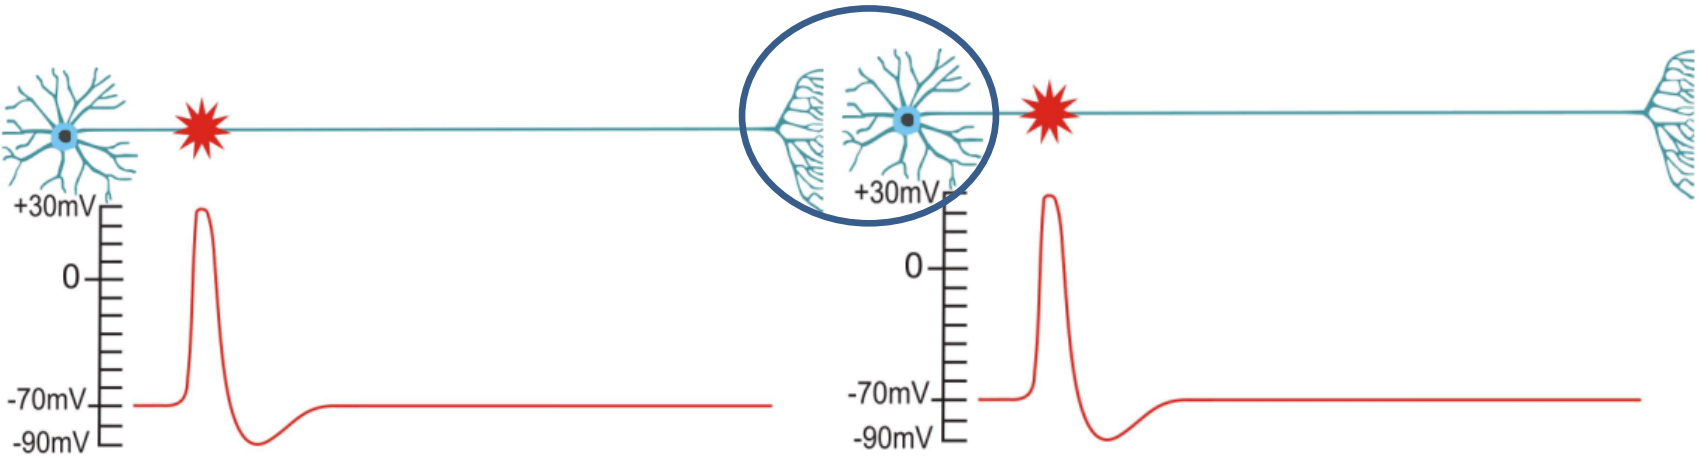
\includegraphics[scale=0.35]{1_1}
    \centering
\end{figure}
Measuring, analyzing, and processing brain signals is done for several reasons, but
the three main ones are listed below:
\begin{itemize}
    \item \textbf{Learn} more about the brain functioning.
    \item \textbf{Mimic} the brain functions in an artificial way - i.e. neuromorphic
    engineering.
    \item \textbf{Employ} brain signals for control and communication, as in the
    case of prosthetics.
\end{itemize}
The nerual code can either be read or written by exploiting several distinct
techniques exhibiting different levels of:
\begin{align*}
    \begin{matrix}
        \textbf{Invasiveness} && \textbf{Risk} &&
        \textbf{Spatial resolution} && \textbf{Temporal resolution}
    \end{matrix}
\end{align*}
The technology nowadays allows fair degrees of spatial and temporal resolution, with
the main reading techniques being fMRI, PET, optical imaging, EEG, ECoG, MEA,
single neuron, and others. Notice that also the number of reading sites is constantly increasing, due to the
exploitation of multiple electrode devices.
\begin{figure}[H]
    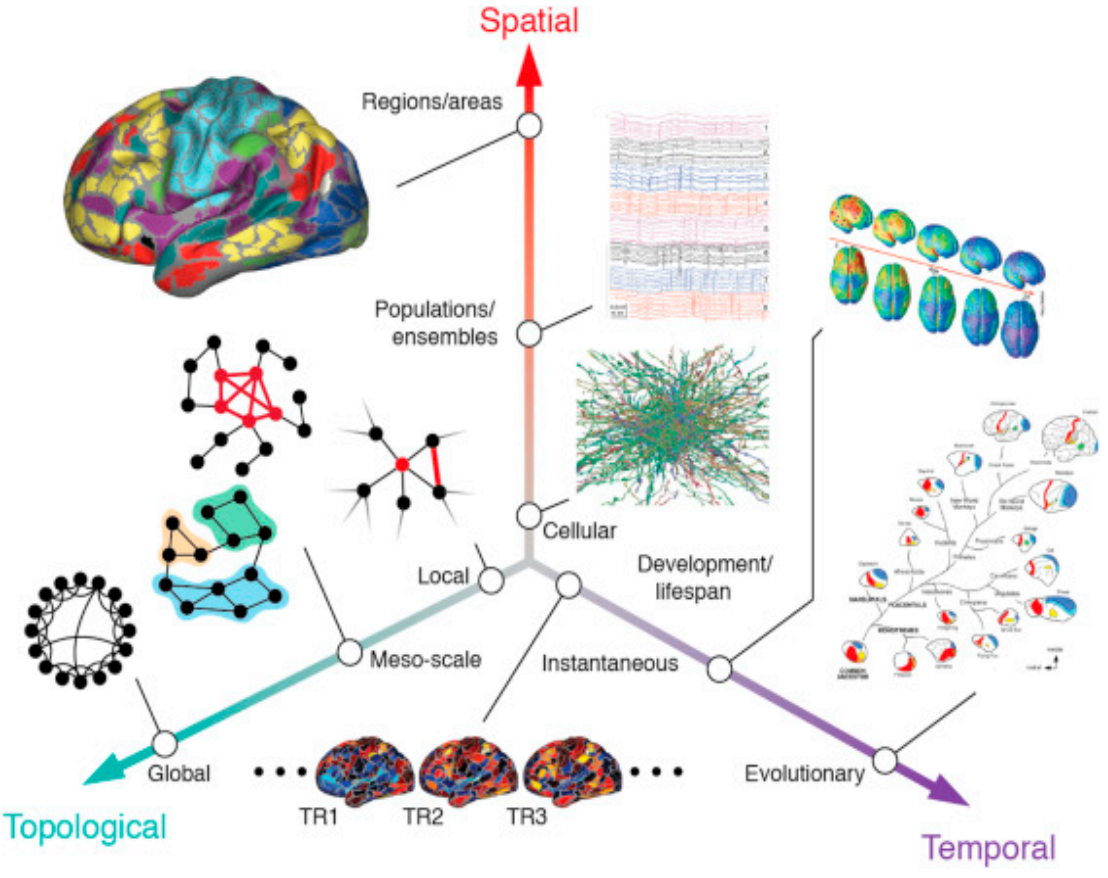
\includegraphics[scale=0.375]{1_2}
    \centering
\end{figure}
The multi-scale brain model presented above aims at showing the different levels at
which the brain activity can be investigated, in terms of spatial, temporal,
and topological scales.
Let's stress once more that the brain can be studied at different level of complexity,
which are somehow related to the risk due to the techniques involved to do so.
\begin{figure}[H]
    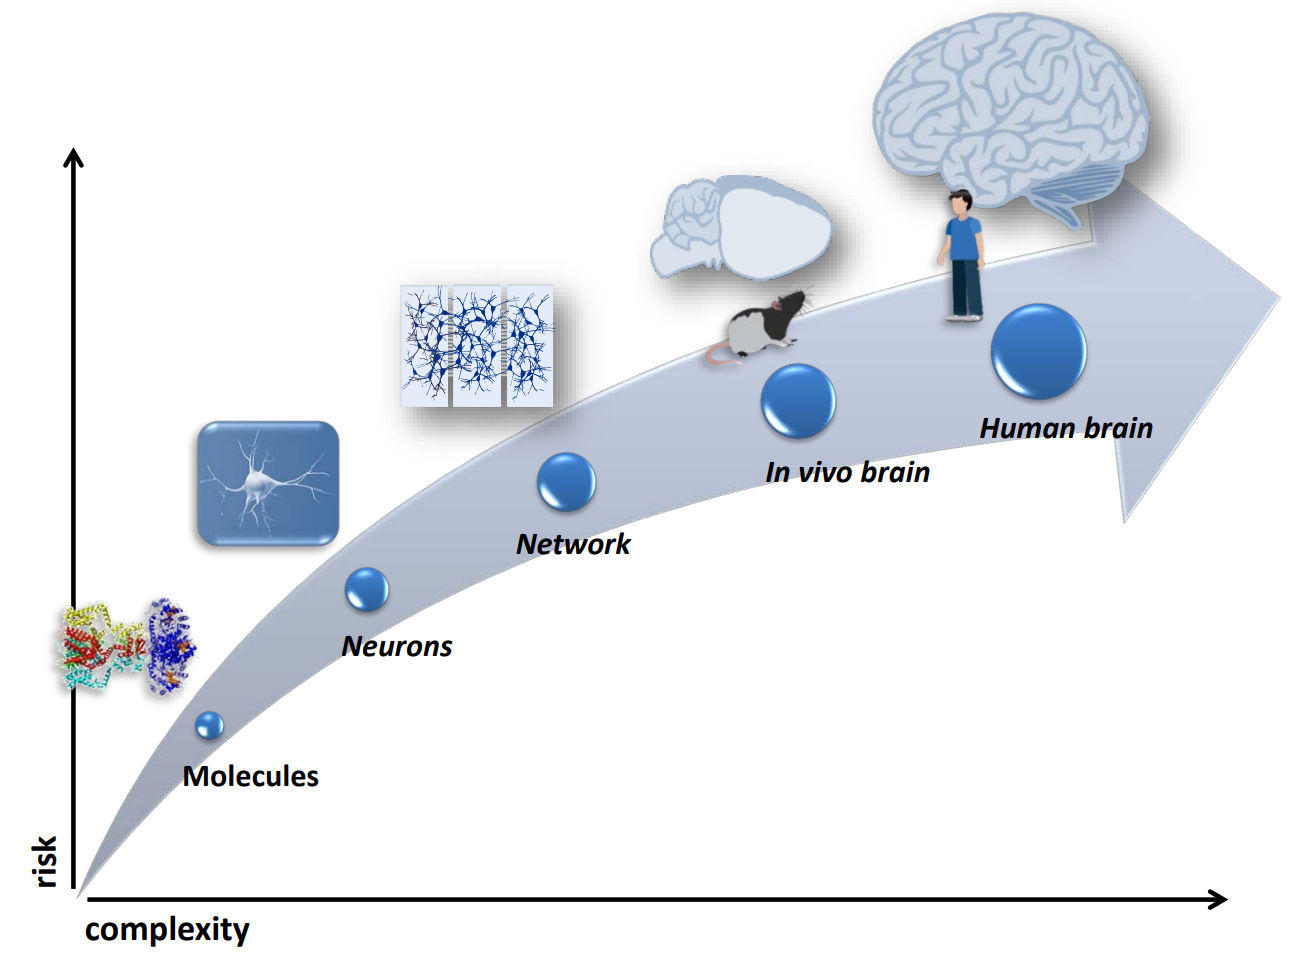
\includegraphics[scale=0.35]{1_3}
    \centering
\end{figure}
Notice that in general the functional unit of the brain is not a single neuron.\\
Two main classes of techniques exist: the in vitro and in vivo ones. Generally, the
second family is more complex to employ, as it requires not to damage the brain of
the experiment subject. One of the principal technologies to study in vitro networks
is MEAs (Micro Electrode Arrays), which are able to detect the activity
of the network at several recording sites and for extended time periods. An issue
related to MEAs is the difficulty often encountered in analysing the recorded data
and interpretating the results in a meaningful way.\\
In general, by recording neural signals at high frequencies and close to few
neurons a signal made of spikes, indicating the firing of a neuron, can be obtained,
while by recording at higher distances the local field potetial (LFP) is instead
obtained, consisting in the low frequency component and accounting for several
neurons as a sort of superposition of their effects.\\
It is common to find in vitro neural networks since they are extensively employed in
research due to their fair level of organization and to the capability to easily
record their activity with arrays of electrodes. Nonetheless, some issues related to
in vitro networks are the fact that they have no fidelity w.r.t. in vivo neurons,
starting from the fact that they generally arranged in 2D layers, instead of
more complex three-dimensional networks.
\begin{figure}[H]
    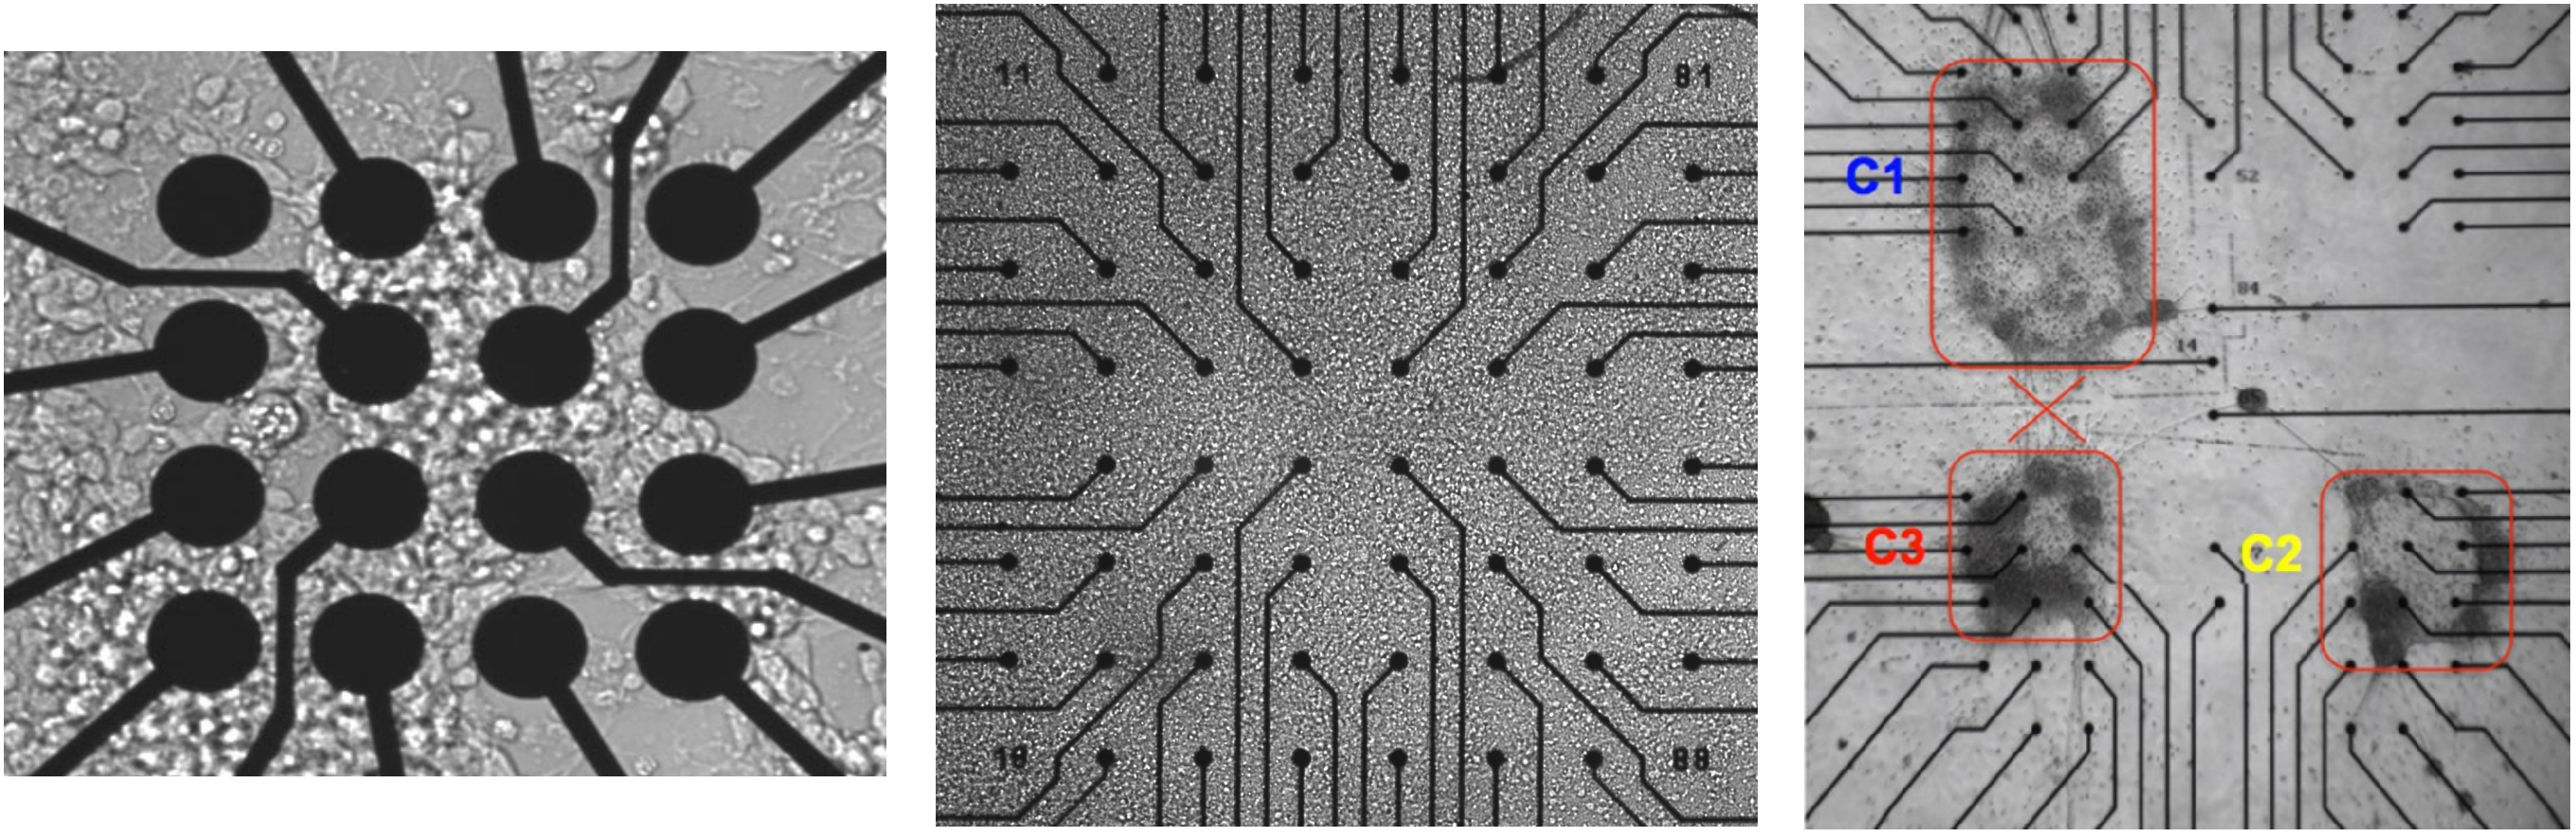
\includegraphics[scale=0.275]{1_4}
    \centering
\end{figure}
Another crucial concept is the one of brain modularity, as a matter of fact the brain
is redundant and intrinsically modular, due to the fact that it is composed of
local networks that are embedded into networks of networks.\\
Other wideley spread techniques are in vitro brain slices and in vivo surgical
procedure. In both cases data are collected from biological tissue by means of
MEAs or similar technologies.\\
The analysis of neural signals is usually performed on spike trains, which are
derived by filtering the raw signal recorded from electrodes and by detecting the
spikes present in it. Notice that the crucial point is not the magnitude of a
certain spike, rather its position on the time axis, indicating when it was fired.
\begin{figure}[H]
    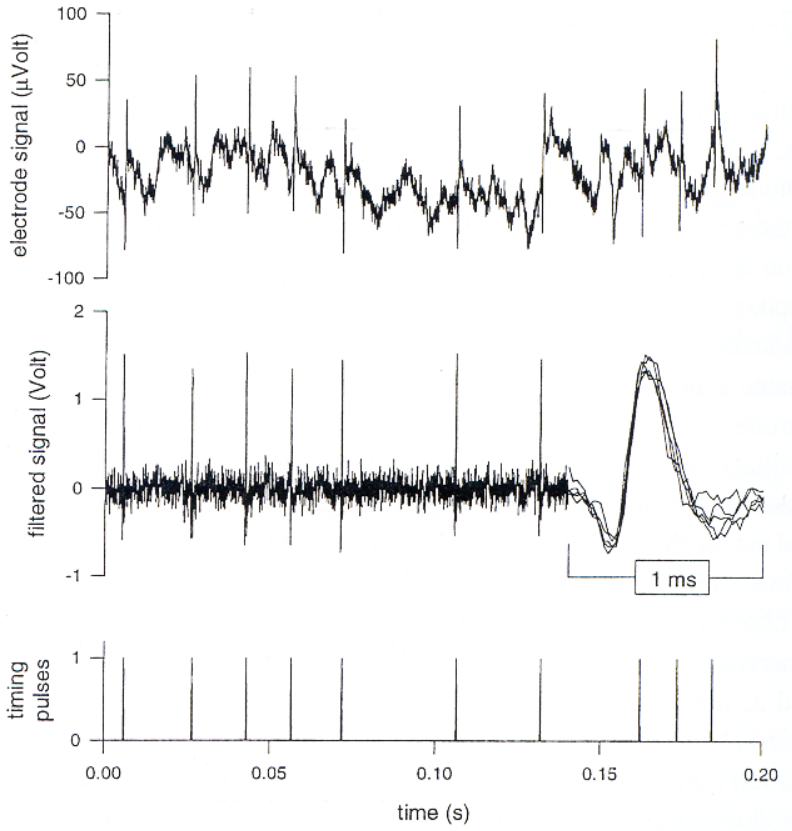
\includegraphics[scale=0.5]{1_5}
    \centering
\end{figure}
It is important to point out that the shape of a spike is highly influenced by the
position of the measuring electrode w.r.t. the neuron that emitted it, enabling
the researchers to recognize all the spikes emitted by the same source - i.e. a
particular neuron - and this is called spike sorting.\\
The main areas of research in this subject are reported in the following list:
\begin{itemize}
    \item Identification and classification of spike events (spike detection and
    spike sorting).
    \item Techniques for measuring the association between neural spike trains.
    \item Quantification of the neural response to a stimulus.
\end{itemize}
Finally, let's highlight that the high number of electrodes employed in today's
research implies a number of new challenges concerning data aquisition, storage,
and analysis.
\newpage

\section{Spike Detection}
\graphicspath{ {./images/2/} }
\subsection{Introduction}
Neural signals are firstly recorded as raw data. They exhibit two main components:
\begin{itemize}
    \item Local field potentials (LFPs) exist at low frequencies (\(0.1-300\,Hz\)).
          \begin{figure}[H]
              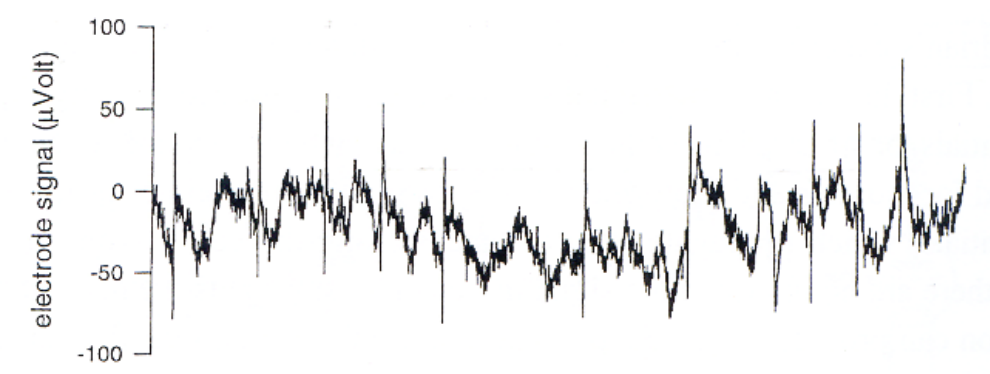
\includegraphics[scale=0.4]{2_1}
              \centering
          \end{figure}
    \item Spikes (MUA) exist at higher frequencies (\(300-3000\,Hz\)).
          \begin{figure}[H]
              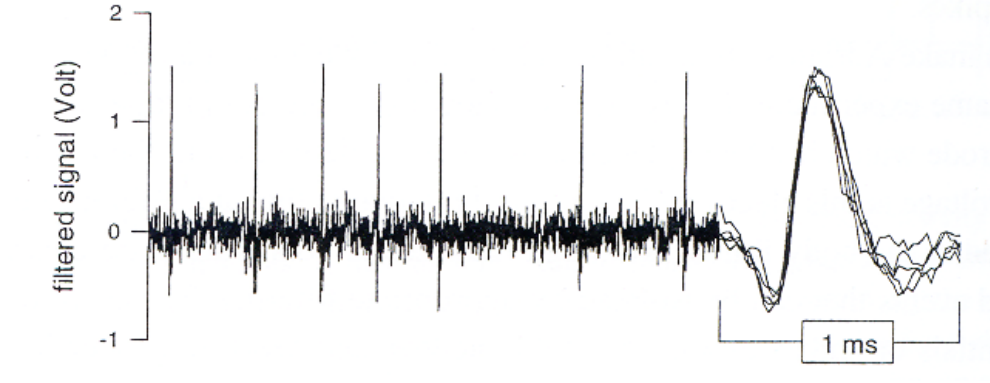
\includegraphics[scale=0.4]{2_2}
              \centering
          \end{figure}
\end{itemize}
The signal is obtained through extracellular recordings, then amplified and filtered. There are 3 possible
situations, according to the distance of the electrode tip from the neurons:
\begin{itemize}
    \item \(<50\,\mu{m}\): the SNR is good enough to distinguish the activity of a
          single neuron (single unit).
    \item \(50\sim150\,\mu{m}\): spikes are still detected, but the difference in their
          shape is masked by the noise (multi-unit activity or MUA).
    \item \(>150\,\mu{m}\): spikes cannot be detected and they contribute to the noise.
\end{itemize}
\begin{figure}[H]
    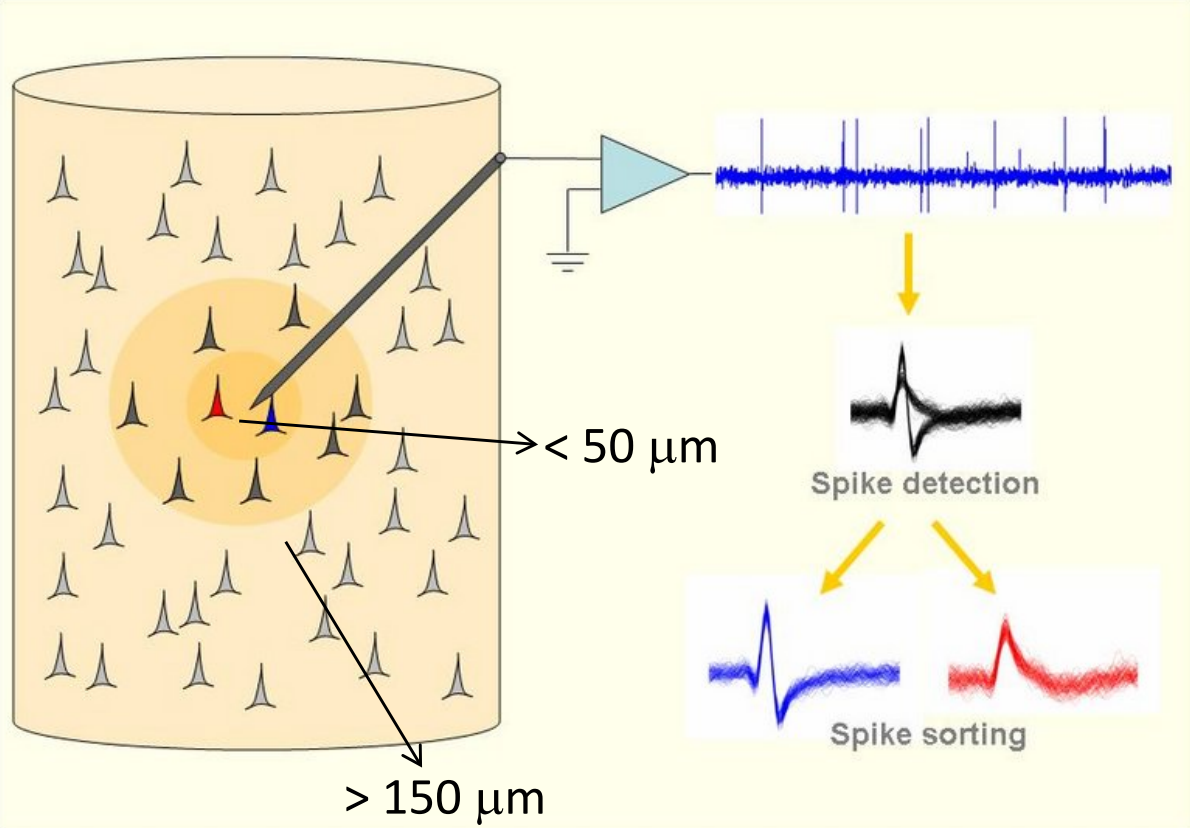
\includegraphics[scale=0.3]{2_3}
    \centering
\end{figure}
The electrophysiological signal, acquired from a single microelectrode is generally
characterized by two different patterns of activity:
\begin{itemize}
    \item \textbf{Spike}: single over-threshold signal representing the
          electrical activity of one or more neurons (1-3 cells).
    \item \textbf{Burst}: sequence of highly packed spikes often occurring simultaneously
          on several channels and giving rise to a phenomenon known as network burst.
\end{itemize}
The workflow commonly followed to preprocess this kind of data is:
\begin{figure}[H]
    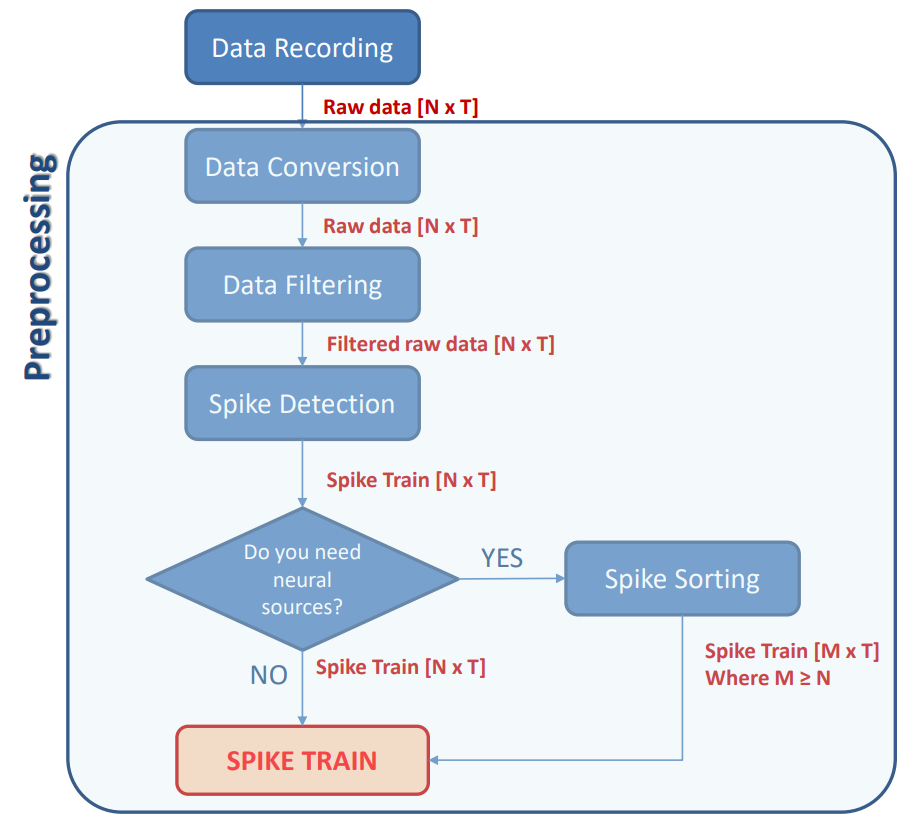
\includegraphics[scale=0.4]{2_4}
    \centering
\end{figure}
\begin{itemize}
    \item \textbf{Data recording:} raw data in the form of a matrix
    \item \textbf{Data conversion:} convert data to a form which is compatible with our system
    \item \textbf{Data filtering:} maintains the dimensionality but filters the data
    \item \textbf{Spike detection:} keeps always the same format (matrix)
    \item \textbf{Take a decision:} is it desirable to identify the individual sources of the signal?
          \begin{itemize}
              \item \textbf{No:} a multi-unit spike train is obtained
              \item \textbf{Yes:} Spike Sorting is performed to retrieve a spike train for
                    every individual source (single unit)
          \end{itemize}
\end{itemize}
Other than the preprocessing part, the other relevant part is the analysis itself, which is performed
by starting from the spike train:
\begin{figure}[H]
    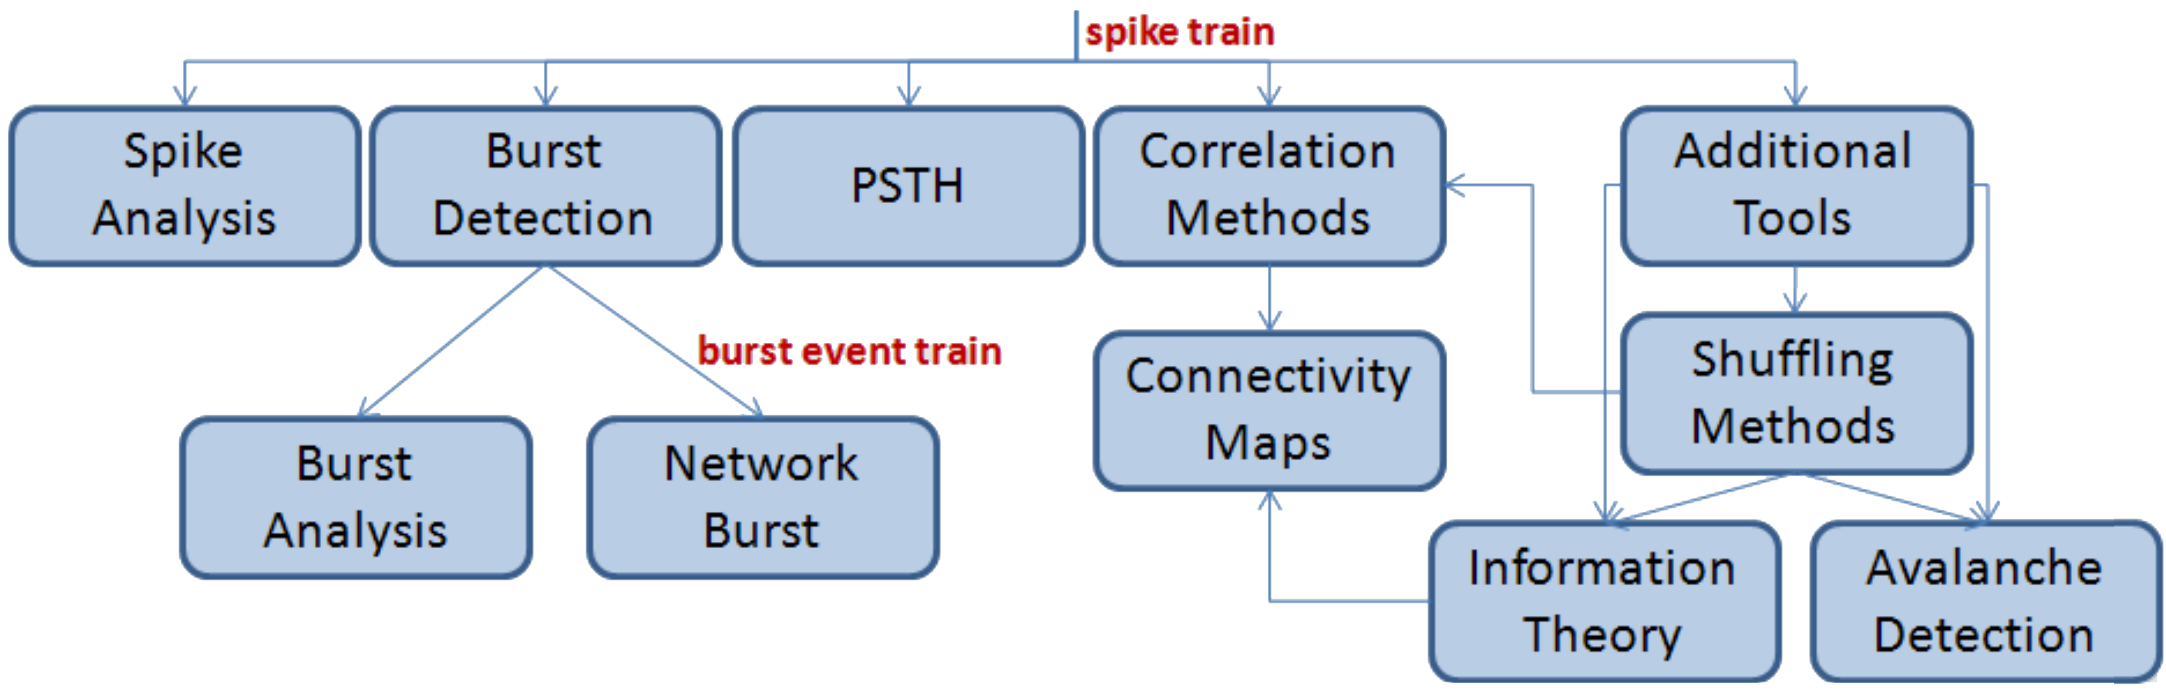
\includegraphics[scale=0.25]{2_5}
    \centering
\end{figure}
As already said, a spike train is a vector containing the positions of spikes with no information
regarding the amplitude (often normalized at \(1\)).
Let's recall the mathematically definition of a spike train:
\begin{itemize}
    \item Single-channel spike train:
          \begin{equation*}
              ST(t)=\sum_{s=1}^{N}\delta{(t-t_s)}
          \end{equation*}
    \item Multi-channel spike train:
          \begin{equation*}
              ST_j(t)=\sum_{s=1}^{N_j}\delta(t-t_s) \hspace{1cm} j=1,\dots,M
          \end{equation*}
\end{itemize}
\begin{figure}[H]
    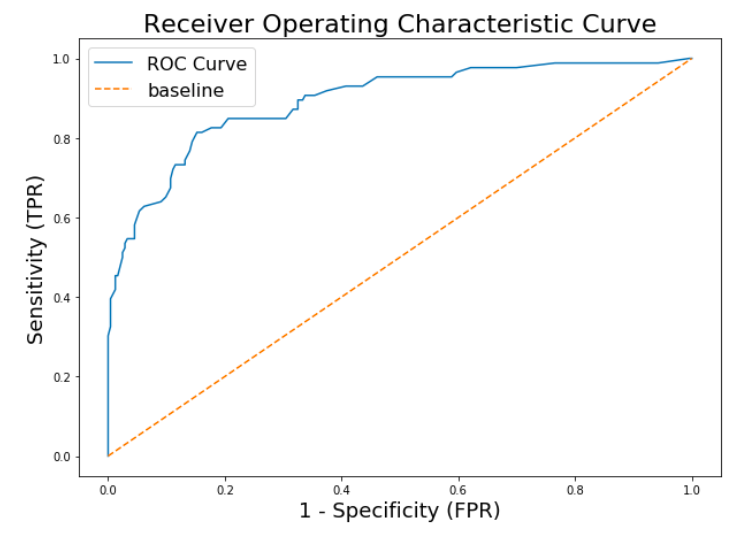
\includegraphics[scale=0.35]{2_6}
    \centering
\end{figure}
\textbf{Spike Detection:} it consists in recognizing the spikes within the raw data. It is the most
important step of the analysis, as it affects all the subsequent steps.\\
\textbf{Spike Sorting:} it is the process of associating each spike to a specific putative source
(classify spikes and individual sources).\\
When performing Spike Detection there are two main issues:
\begin{itemize}
    \item \textbf{Reliability} of the selected detection method
    \item \textbf{Precise position} of the detected peaks in the spike train
\end{itemize}

\subsection{Spike Detection algorithms}
So far, many algorithms have been developed but none of them has emerged as the best one yet.
They can be classified into 3 groups:
\begin{itemize}
    \item \textbf{Thresholding}: it is assumed that spikes peak-to-peak amplitude is larger than the noise level.
    \item \textbf{Energy operator}: non-linear energy operator accentuating high frequency content, i.e., spikes.
    \item \textbf{Template matching}: it is an approach based on the spike shape, involving Spike Sorting.
\end{itemize}
\subsubsection{Thresholding algorithms}
\paragraph{Simple Hard Threshold}
A \textbf{threshold} value is defined (either positive or negative). If the signal overcomes the threshold,
then a spike is detected. A \textbf{refractory period} (\(RP\)) between two peaks is employed to account for
subsequent samples overcoming the threshold after a spike detection.\\
Simple hard thresholding is characterized by a very simple logic and for this reason it is often employed in
commercial systems for data acquisition where the online detection of the spikes is required. This kind of
detection technique is often useful because it is quite fast, even if at the expenses of precision.
\begin{figure}[H]
    \centering
    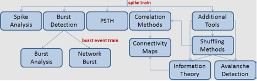
\includegraphics[scale=0.22]{2_7.png}
\end{figure}
\paragraph{Hard Threshold} Notice this algorithm is applied also to absolute-valued
signals. It involves 2 distinct main steps: application of a threshold and spike identification.\\
A time window denoted by \(T\) is applied to the signal, centering the window \(\frac{1}{3}T\) before the detected spike.
The length of \(T\) is to be carefully chosen, usually it is between \(1\) and \(3\,ms\), as it must minimize the likelihood
that more than one spike is captured in the window.\\
The threshold (\(Thr\)) can be defined in several ways:
\begin{itemize}
    \item \(Thr=n\sigma[V]\): \(n\) times the standard deviation \(\sigma\) of the basal signal noise.
    \item \(Thr=aP2P[V]\): fraction of the full amplitude (peak-to-peak) of the signal.
    \item \(Thr=n\sigma_N[V]\): \(n\) times the \(\sigma\) estimated from the
          Median Absolute Deviation (\(MAD\)), with \(MAD=median(|x-median(x)|)\) and \(\sigma_N=1.4826\cdot MAD\).
          A good value for \(n\) is \(4\).
\end{itemize}
\paragraph{Hard Threshold Local Maxima}
This method is very similar to the previous ones, but in this case the spike position is
associated to the local maxima (and not set at the time of the first sample overcoming the threshold).
\begin{figure}[H]
    \centering
    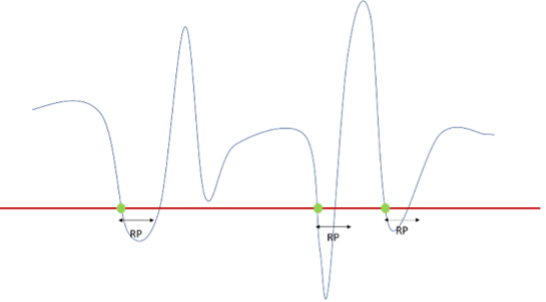
\includegraphics[scale=0.2]{2_8.png}
\end{figure}
\paragraph{Hard Threshold Differential Threshold}
A sliding window \(W\) is sized to contain at least one spike and is shifted over the signal.
The peak-to-peak threshold \(k\sigma\) is a multiple of the noise standard deviation (usually \(k=7\) or \(8\)).
A spike is detected in the \(i-\)th window when
\begin{equation*}
    [(max_i-min_i)\ge{k\sigma}]
\end{equation*}
with \(i=1,\dots,\frac{T}{W}\) and \(T\) being the entire duration of the signal.\\
This approach exhibits a major issue, which is related to undersampling if more spikes are found
in a single window (typically at the window borders).
\begin{figure}[H]
    \centering
    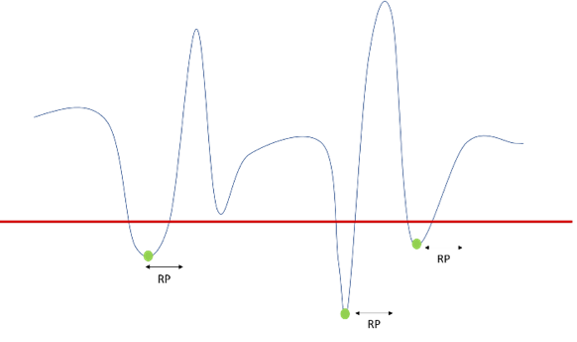
\includegraphics[scale=0.18]{2_9.png}
\end{figure}
\paragraph{Precision Timing Spike Detection (PTSD)}
This method solves the undersampling issue. \\ The operation of PTSD differs from the previous
algorithms in a variety of aspects: first and foremost, the presence of a differential threshold
instead of a unipolar one; moreover, in addition to \(RP\), there is also another time interval
called \textbf{Peak Lifetime Period} \(PLP\) - i.e., the maximum duration that a spike can have -.
\begin{figure}[H]
    \centering
    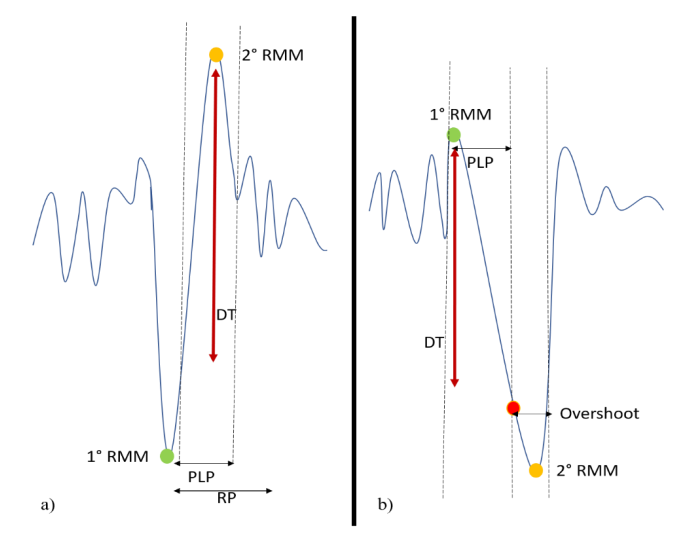
\includegraphics[scale=0.3]{2_10.png}
\end{figure}
Proceeding in order, the algorithm searches for a relative maximum/minimum (\(1^\circ\) \(RMM\),
Relative Maximum/Minimum): if it finds a maximum then it will search the signal for
the nearest minimum (\(2^\circ\) \(RMM\)) within the \(PLP\) window, while if it finds a minimum it will proceed
in the same way but looking for a maximum. If the difference between the first \(RMM\) and the second \(RMM\)
- i.e., the peak-to-peak amplitude of the spike -, exceeds the Differential Threshold (\(DT\)),
then the spike is identified (\textit{Fig. a}). In case the second \(RMM\) falls at the end of the \(PLP\) window,
another time window called \textbf{overshoot} is used to find the correct peak value (\textit{Fig. b}). The \(DT\) is
always calculated as the standard deviation of the noise multiplied by a coefficient.\\
Of course, this algorithm can't be used in real time, because it needs future times, but it allows to detect also the
spikes passing through the boundaries of the considered window.
This technique is more demanding from the computational point of view, but it allows to detect
also the spikes passing through the boundaries of the considered window.
\subsubsection{Energy operator algorithms}
\paragraph{Signed Energy (SE)}
The SE algorithm is based on a moving window, whose width is set by the user,
which is used to scan the signal. For each time point, centered on the window width,
the energy is given by the sum of the squares of the voltage amplitudes within the
window, averaged by the window width:
\begin{equation*}
    SE(i)=\frac{1}{W}\sum_{j=i-\frac{W}{2}}^{j+\frac{W}{2}}V(j)^2
\end{equation*}
where \(V\) are the voltage amplitudes within the window and \(W\) is the window width.\\
The result is then multiplied by \(+1\) when the average amplitude of the raw signal is positive,
by \(-1\) when negative.\\
Since this algorithm has been implemented in the Offline Sorter commercial software,
we refer to it also as Offline Sorter Signed Energy (OSSE).
\paragraph{Nonlinear Energy Operator (NEO)}
The NEO algorithm is defined such that:
\begin{itemize}
    \item Constant voltage or zero \(\Rightarrow NE=0\)
    \item Waveform rapidly varying and a large amplitude \(\Rightarrow NE \text{ is maximum}\).
\end{itemize}
The \(NE\) of a signal \(x(n)\) is defined as:
\begin{align*}
    \psi[x(n)]=x^2(n)-x(n+1)\cdot x(n-1)
\end{align*}
The NEO is defined for each sample \(i\) and computed within a
window \(W\) centered in \(i\).\\
As a consequence, the NEO is large only when the signal is both high in power - i.e., \(x^2(n)\) is large -
and high in frequency - i.e., \(x(n)\) is large while \(x(n+1)\) and \(x(n-1)\) are small-.
Since a spike is characterized by localized high frequencies and an increase in instantaneous energy,
this method has an obvious advantage over methods that look only at an increase in signal energy or
amplitude without regarding the frequency.\\
The threshold is set to a scaled version of the mean of the NEO
\begin{align*}
    Thr=C\frac{1}{N}\sum_{n=1}^{N}\psi[x(n)]
\end{align*}
where \(N\) is the number of samples in the signal and \(C\) a scaling factor,
experimentally determined as \(C=8\).\\
If a smoothing window is applied after the NEO computing, the algorithm takes the name of smoothing NEO (SNEO).

\subsection{Assessing the Quality of a Spike Detection Method}
\subsubsection{Groundtruth}
In order to assess the performance of a Spike Detection algorithm, a groundtruth has to
be defined, such that several metrics of the tested algorithm can be computed.
A \textbf{groundtruth} is a collection of information (typically a dataset)
which is known to be true, opposed to information provided by inference.
There are 3 main types of groundtruths:
\begin{itemize}
    \item \textbf{Experimental groundtruth}: neurons are recorded into two distinct ways,
          extracellular and intracellular (or juxtacellular). Then a researcher uses the
          precise intracellular recordings (exhibting precise timing and localization) to find
          the same spikes into the extracellular signal.
    \item \textbf{Computational groundtruth}: data are synthetic and generated by a model
          reproducing the behaviour of a network of neurons under different conditions.\\
          In particular, this method enables the researcher to test the Spike Detection
          algorithms against datasets with different characteristics, such as different
          signal-to-noise ratios (SNR). This comparison using SNR can help to understand if
          the tested algorithm is reliable: if the peaks are identifiable also in bad
          conditions of SNR, then it is good.\\
          Notice that the SNR can be computed as the ratio of the mean of the peak to peak
          amplitude between all the spikes over 6 times the minimum noise standard deviation
          (evaluated in 10 different random intervals):
          \begin{equation*}
              SNR = \sqrt{\frac{\frac{1}{N}\sum_{i=1}^N(P2P_{up})_i}{6\sigma_{noise}}}
          \end{equation*}
    \item \textbf{Hybrid groundtruth}: natural and synthetic data are mixed.
          In particular, it is common to exploit manually detected and sorted spikes to be
          fed into computational models as input.
\end{itemize}
\subsubsection{Spike Detection Performance Evaluation}
Several distinct metrics can be taken into account when evaluating the performance of
a Spike Detection algorithm, in particular the most used ones are:
\begin{itemize}
    \item \textbf{Error count:}
          \begin{itemize}
              \item Type I error \(\Rightarrow\) False Positive (FP): incorrect
                    inclusion of noise, or spikes or other cells.
              \item Type II error \(\Rightarrow\) False Negative (FN): inability to
                    detect actual spikes.
          \end{itemize}
    \item \textbf{Position (mean) error:} the position of the
          detected spike is compared to the model one (mean error)
    \item \textbf{ROC curve}
\end{itemize}
\paragraph{Example} Hard Threshold algorithm errors\\
\begin{figure}[H]
    \centering
    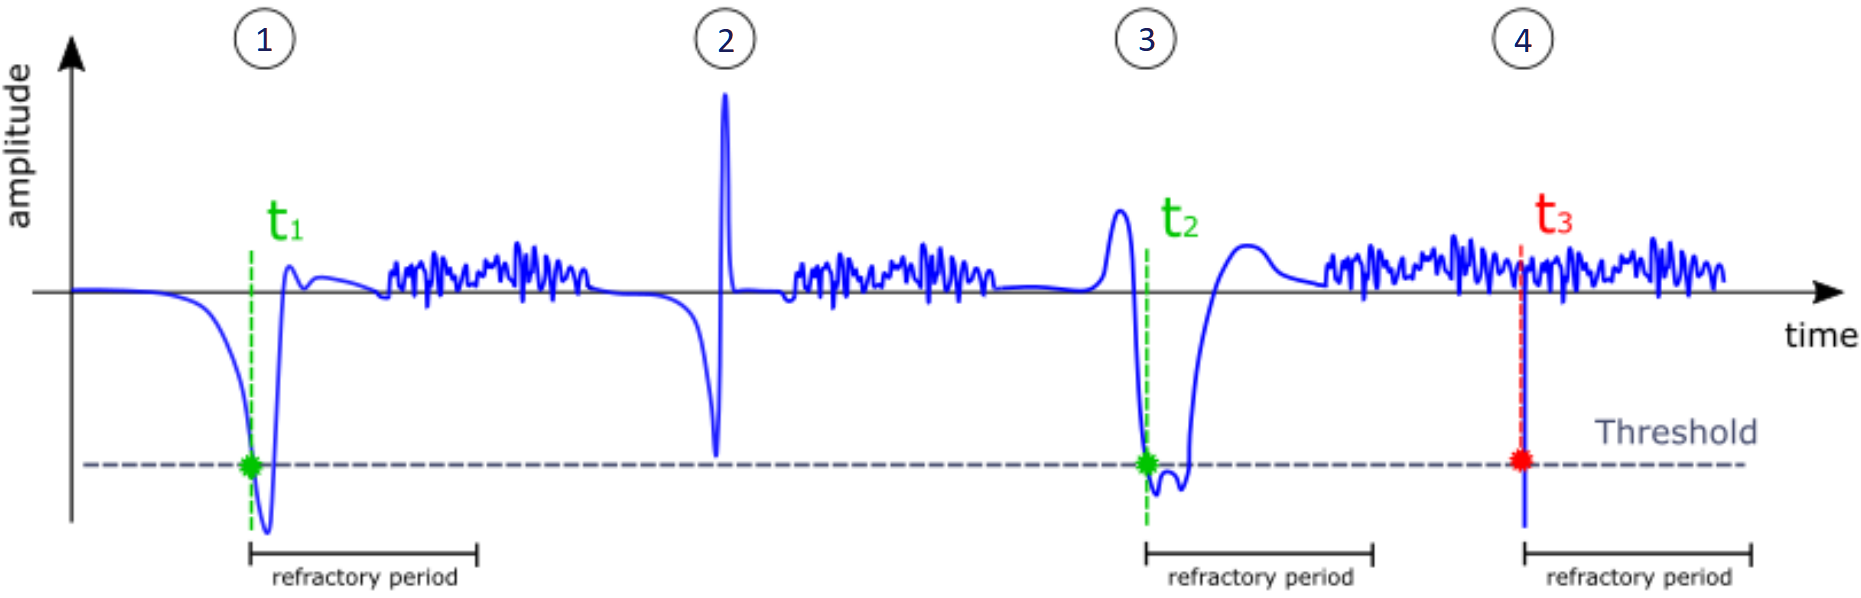
\includegraphics[scale=0.3]{2_11}
\end{figure}
\begin{enumerate}
    \item \textbf{True positive:} the algorithm detects all the samples above the threshold
          identifying as a spike position the first one, therefore the refractory period begins.
    \item \textbf{False negative:} if a spike occurs under the threshold, the algorithm
          misses it.
    \item \textbf{True positive:} the refractory period additionally helps to avoid the
          detection of double peaks which occasionally can occur in neural recordings.
    \item \textbf{False positive:} if some noise overcomes the threshold,
          a wrong spike is detected.
\end{enumerate}
A spike belonging to the spike train obtained from the tested algorithm is said to
have a \textbf{corresponding spike} in the groundtruth reference spike train if their
time distance is less than a defined threshold and no other spikes occur within
this time window.\\
Let's define the following variables:
\begin{itemize}
    \item \(NREF\): number of reference spikes (true spikes present in the groundtruth
          dataset)
    \item \(NDS\): number of detected spikes (spikes identified by the tested Spike
          Detection algorithm)
    \item \(NCS\): number of corresponding spikes (spikes correctly identified by
          the algorithm matching the groundtruth data)
\end{itemize}
The following expressions for False Positives and False Negatives can be derived:
\begin{align*}
    \text{\textbf{False Positives}}\Rightarrow FP=NDS-NCS
    \quad\quad\quad
    \text{\textbf{False Negatives}}\Rightarrow FN=NREF-NCS
\end{align*}
\begin{figure}[H]
    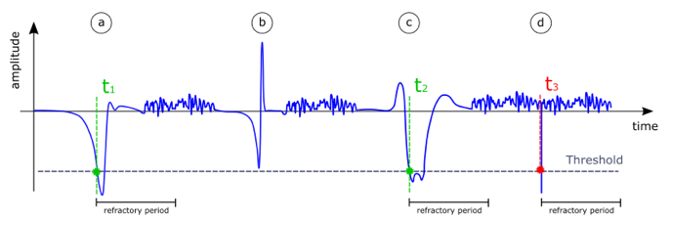
\includegraphics[scale=0.25]{2_12}
    \centering
\end{figure}
\paragraph{Receiver Operating Characteristics} The ROC curve is a well-known technique
for visualizing, organizing and selecting classifiers based on their performance.
In order to reduce the ROC performance to a single scalar indicator comprised between 0 and 1,
it is possible to calculate the Area Under the ROC Curve (AUC).\\
Notice that the ROC curve provides information regarding False Positives, but nothing
is said about False Negatives.
\paragraph{Confusion Matrix} This matrix is special type of contingecy matrix and
it allows to visualize the performance of an algorithm. Each row of the matrix
represents the instances in an actual class while each column represents the instances
in a predicted class (or vice versa). The confusion matrix term comes from the fact that
such a visualization allows to assess whether the system is confusing two classes.
\begin{figure}[H]
    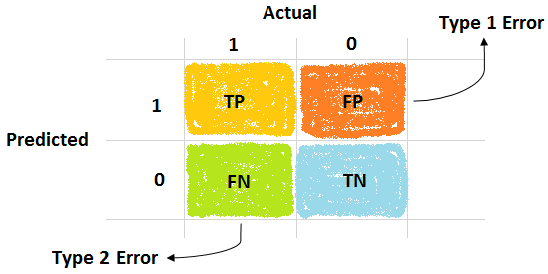
\includegraphics[scale=0.20]{2_13}
    \centering
\end{figure}
\paragraph{Other Metrics} Other useful metrics are introduced in the following.
\begin{align*}
    \begin{matrix}
        TP_{rate}   &  & \frac{Positives\,Correctly\,Classified}{Total\,Positives}=\frac{TP}{P}                 \\\\\\
        FP_{rate}   &  & \frac{Negatives\,Incorrectly\,Classified}{Total\,Negatives}=\frac{FP}{N}=1-Specificity \\\\\\
        Sensitivity &  & \frac{TP}{TP+FN}=\frac{TP}{P}=TP_{rate}                                                \\\\\\
        Specificity &  & \frac{TN}{TN+FP}=\frac{TN}{N}                                                          \\\\\\
        Accuracy    &  & \frac{TP+TN}{P+N}                                                                      \\\\\\
        Performance &  & \eta=\frac{TP}{FP+FN}                                                                  \\\\\\
        Efficiency  &  & \eta_2=\frac{\eta}{\eta+1}=\frac{TP}{TP+FN+FP}=\frac{TP}{P+FP}
    \end{matrix}
\end{align*}

\newpage

\section{Spike Sorting}
\graphicspath{ {./images/3/} }
\subsection{Introduction}
\textbf{Spike Sorting} can be defined as the grouping of spikes into clusters according
to the similarity of their shapes.\\
It is useful only if the following assumption is made: each neuron tends to fire spikes
with a peculiar (distinguishable) extracellular shape.
As a consequence, it is possible to determine the activity of each one of these neurons
according to the measured spikes associated with it through Spike Sorting.\\
There are 3 main reasons for which Spike Sorting useful:
\begin{itemize}
    \item \textbf{Increase the scale}: as modern devices (MEAs) record from large
          populations of neurons at the same time, it is desirable to derive the individual
          activity of as many neurons as possible.
    \item \textbf{Carry out new types of analysis}: it might be interesting to study
          connectivity patterns of close-by neurons or perform analysis at single-neuron
          level.
    \item \textbf{Have access to sparsely firing neurons}: it is desirable to understand
          the typical patterns of a specific kind of neuron, allowing to study its specific
          function.
\end{itemize}
Despite everything, Spike Sorting still presents a number of major problems:
\begin{itemize}
    \item Dealing with background noise.
    \item Neurons in the same area might produce spikes with a similar shape (there is
          no way to perfectly know which neuron fired apart from imaging techniques).
    \item Neurons in the same area might emit spikes with a smaller amplitude.
    \item Background activity of distant neurons pollutes the recorded signal.
    \item Waveform misalignment.
    \item Variation of the spike shape as a function of recent firing history
          (not time-invariant shape).
\end{itemize}
\begin{figure}[H]
    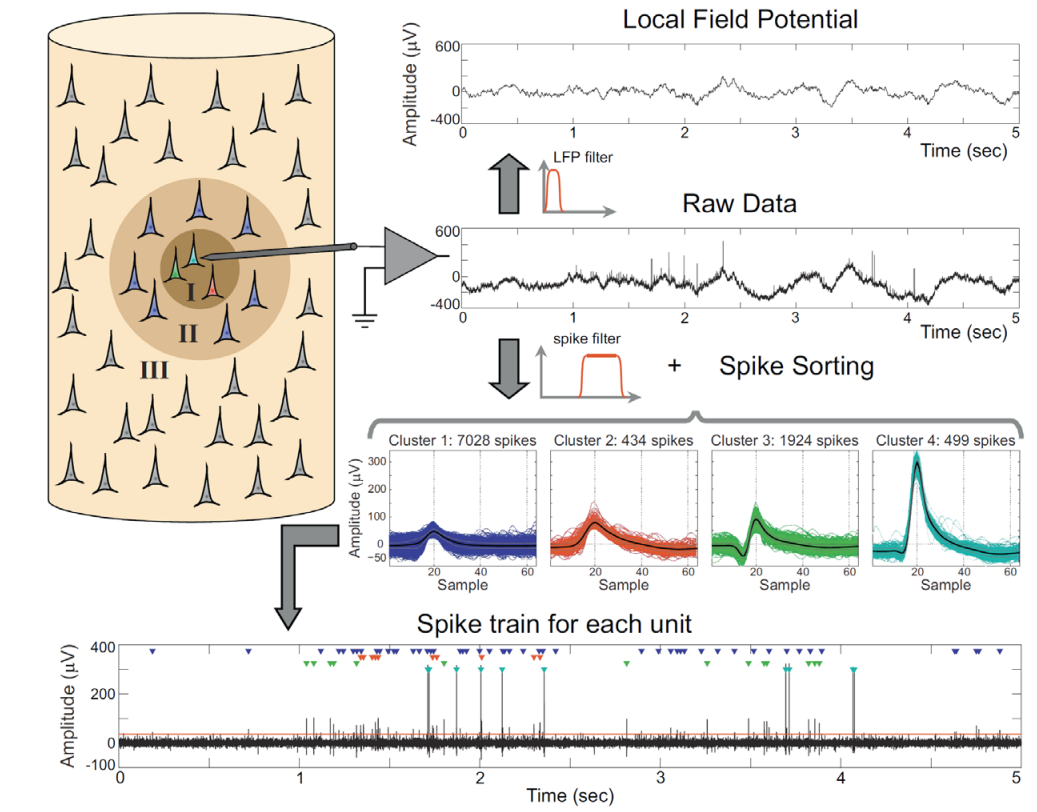
\includegraphics[scale=0.35]{3_1}
    \centering
\end{figure}

\subsection{Spike Sorting methods}
When it comes to Spike Sorting, there are three main approaches:
\begin{itemize}
    \item \textbf{Amplitude discriminator}: separate spikes according to their amplitude.
          This method does not take into account the shape of a spike, only its amplitude.\\
          \textit{Main problem:} spikes from different neurons may have the same peak
          amplitude but different shapes.
    \item \textbf{Template matching}: select a characteristic spike shape for each
          cluster and divide the spikes among the clusters via matching with the templates,
          according to an appropriate distance measure.\\
          \textit{Main problems:} the templates might need to be adjusted during the
          experiment and it is necessary a good way to select them in the first place.
    \item \textbf{Window discriminator}: assign spikes crossing one or more windows to
          the same neurons.\\
          \textit{Main problem:} it requires manual setting by the user and it is not
          suitable for many channels and subjectivity. Moreover, spikes may overlap: it may
          be difficult to set windows for discrimination and sparsely firing neurons may be
          missed.
\end{itemize}
Please note that these algorithms perform Spike Detection and Spike Sorting at the same
time.\\
\subsection{Spike Sorting steps}
In general, Spike Sorting is carried out by following the steps shown below:
\begin{figure}[H]
    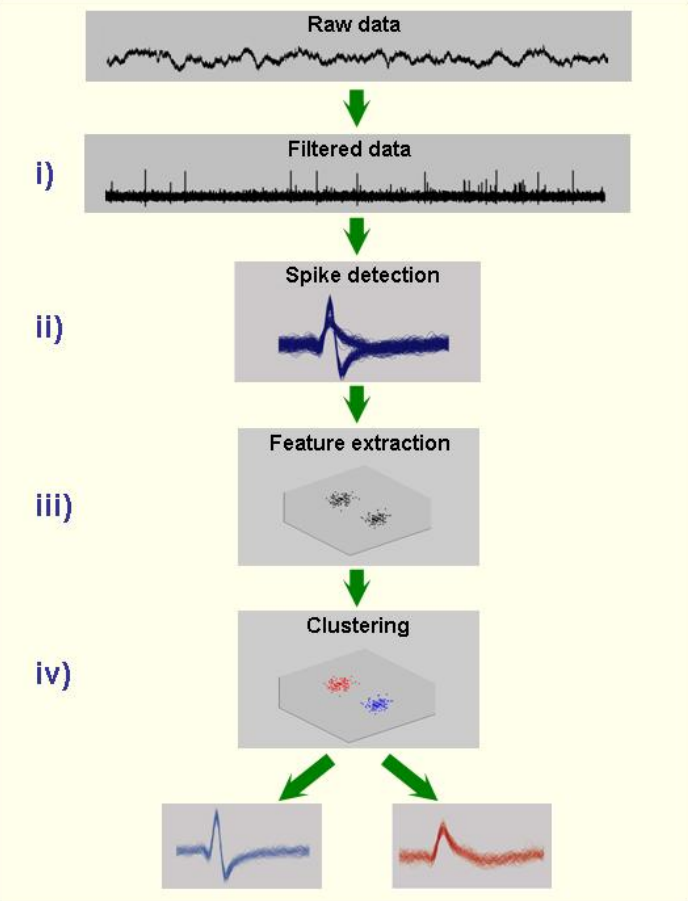
\includegraphics[scale=0.4]{3_2}
    \centering
\end{figure}
\subsubsection{Filtering}
The first step consists in filtering out the low frequency components (\(< 300 \,Hz\)),
in particular the local field potentials, in order to visualize spikes. To do so, a
\(300-3000 \,Hz\) band-pass filter is employed: all the frequencies outside the
specified range are rejected.
\begin{figure}[H]
    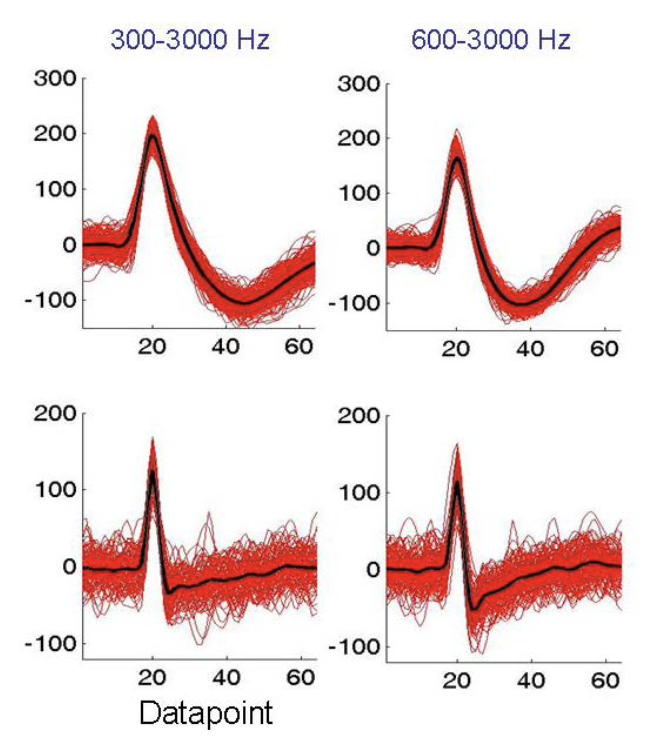
\includegraphics[scale=0.4]{3_3}
    \centering
\end{figure}
\subsubsection{Spike Detection}
Spikes are commonly detected by using an amplitude threshold, as seen in the previous
chapter. The optimal threshold can be set manually or automatically computed as a
multiple of the standard deviation \(\sigma\) of the signal:
\begin{equation*}
    \sigma=median\biggl(\frac{|x|}{0.6745}\biggr)
\end{equation*}
\subsubsection{Feature Extraction}
Let's set the number of observations - i.e. spikes - to \(n\) and the variables
(data points) to \(m\), thus a \(m\)-dimensional space is obtained. The idea is to
extract a number of features \(p\), such that \(p<m\). In this way the signal is
described with a decreased number of features with respect to the original ones.\\
The \(p\) features can be selected by:
\begin{itemize}
    \item Taking some basic properties of the spikes (amplitude, width, energy, ...),
          but they might not be optimal in differentiating spikes.
    \item Selecting a low number of components from a dimensionality reduction
          technique, such as \textbf{PCA}. Notice that these components represent the
          directions of maximum variance of the data, not necessarily the best separation.
    \item Using \textbf{wavelets}, obtaining a time-frequency decomposition of the
          signal with optimal resolution in both time and frequency domains.
\end{itemize}
\paragraph{Principal Component Analysis (PCA)}
It is an unsupervised dimensionality reduction technique, which can be used also for
feature extraction purposes. Data are rotated according to a new space having the
orthogonal axes in the directions of maximum variance, then the new obtained principal
components are ordered by their contribution to the overall variance, allowing to
select only a fraction of the total number of components, still approximating the
original data fairly well. Low variance is often interpreted as background noise.\\
The dimensionality of the data can therefore be reduced, without the loss of relevant
information, by extracting a lower dimensional space still ensuring a fairly high variance.
\begin{figure}[H]
    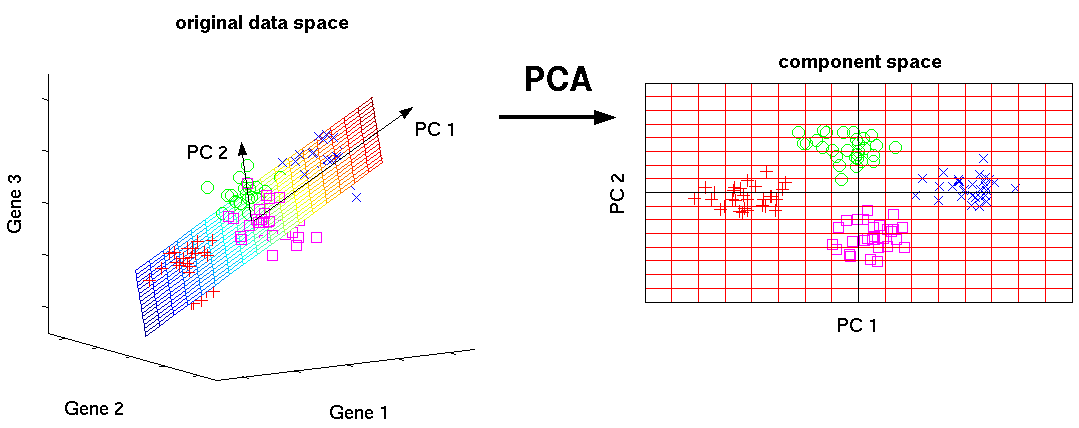
\includegraphics[scale=0.45]{3_4}
    \centering
\end{figure}
\paragraph{Wavelets}
The wavelet transformation (WT) is a joint time-frequency representation of the signal.
When compared to other more spread methods, it has the main advantage to provide an
optimal resolution in both the time and the frequency domains.\\
The wavelet analysis is similar to the windowed Fourier analysis in the sense that it breaks a
signal down into its constituent parts. However, whereas the Fourier transform breaks the
signal into a series of sine waves of different frequencies, the wavelet transform breaks
the signal into its wavelets, which are scaled and shifted versions of a parametric "mother"
wavelet. Notice that sines and cosines are infinite in time, while a wavelet must exhibit
a local support, indicating that it is finite in time.\\
The Wavelet transform may be defined as the convolution between the signal \(x(t)\) and the
wavelet function \(\psi_{a,b}(t)\):
\begin{align*}
    W_\psi X(a,b)=\left\langle x(t)|\psi_{a,b}(t) \right\rangle\hspace{0.5cm}\text{with}\hspace{0.5cm}\psi_{a,b}(t)=|a|^{-\frac{1}{2}}\psi\biggl(\frac{t-b}{a}\biggr)
\end{align*}
where \(a\) and \(b\) are scale and translation parameters.\\
A tight wavelet function will match the high-frequency components, while a dilated wavelet
will match the low-frequency ones, thus details of the signal at several scales are obtained.
\begin{figure}[H]
    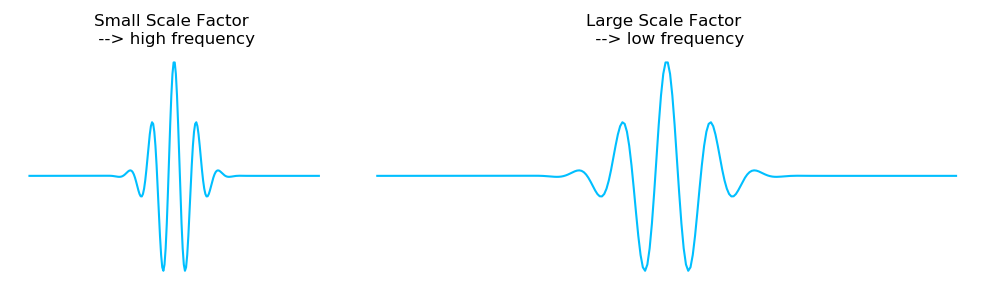
\includegraphics[scale=0.25]{3_5}
    \centering
\end{figure}
When employing wavelets, the information about the shape of the spikes is distributed
in several coefficients, not just in 2-3 PCs as it happens for PCA. A wavelet
coefficient (or any other feature) in order to be effective in distinguishing spike
shapes should have a multi-modal distribution, unless there is only one cluster.
\subsubsection{Clustering}
The final step of spike sorting consists in grouping together the spikes with similar
features into clusters, corresponding to different neurons. Different approaches are
available:
\begin{itemize}
    \item Manual clustering
    \item Bayesian classification
    \item Expectation-Maximization methods
    \item Hierarchical clustering
    \item K-Means
    \item Superparamagnetic clustering
\end{itemize}
\paragraph{K-means Clustering}
K-means clustering is a partitioning method that treats each observation in the data as
an object having a location in the space. It finds a partition in which objects within
each cluster are as close as possible, while object in different clusters should be as
far apart as possible.\\
Each cluster in the partition is defined by its members and by its centroid.
The centroid of each cluster is computed as the mean position of all the cluster members,
which are partitioned among the available clusters in order to minimize the sum of
the distances from the centroid itself.\\
It is quite important that the user sets the correct number of  desired clusters
(initial centroids can be specified as well).\\
Notice that this method works well with spherical and similarly scattered clusters.
\begin{figure}[H]
    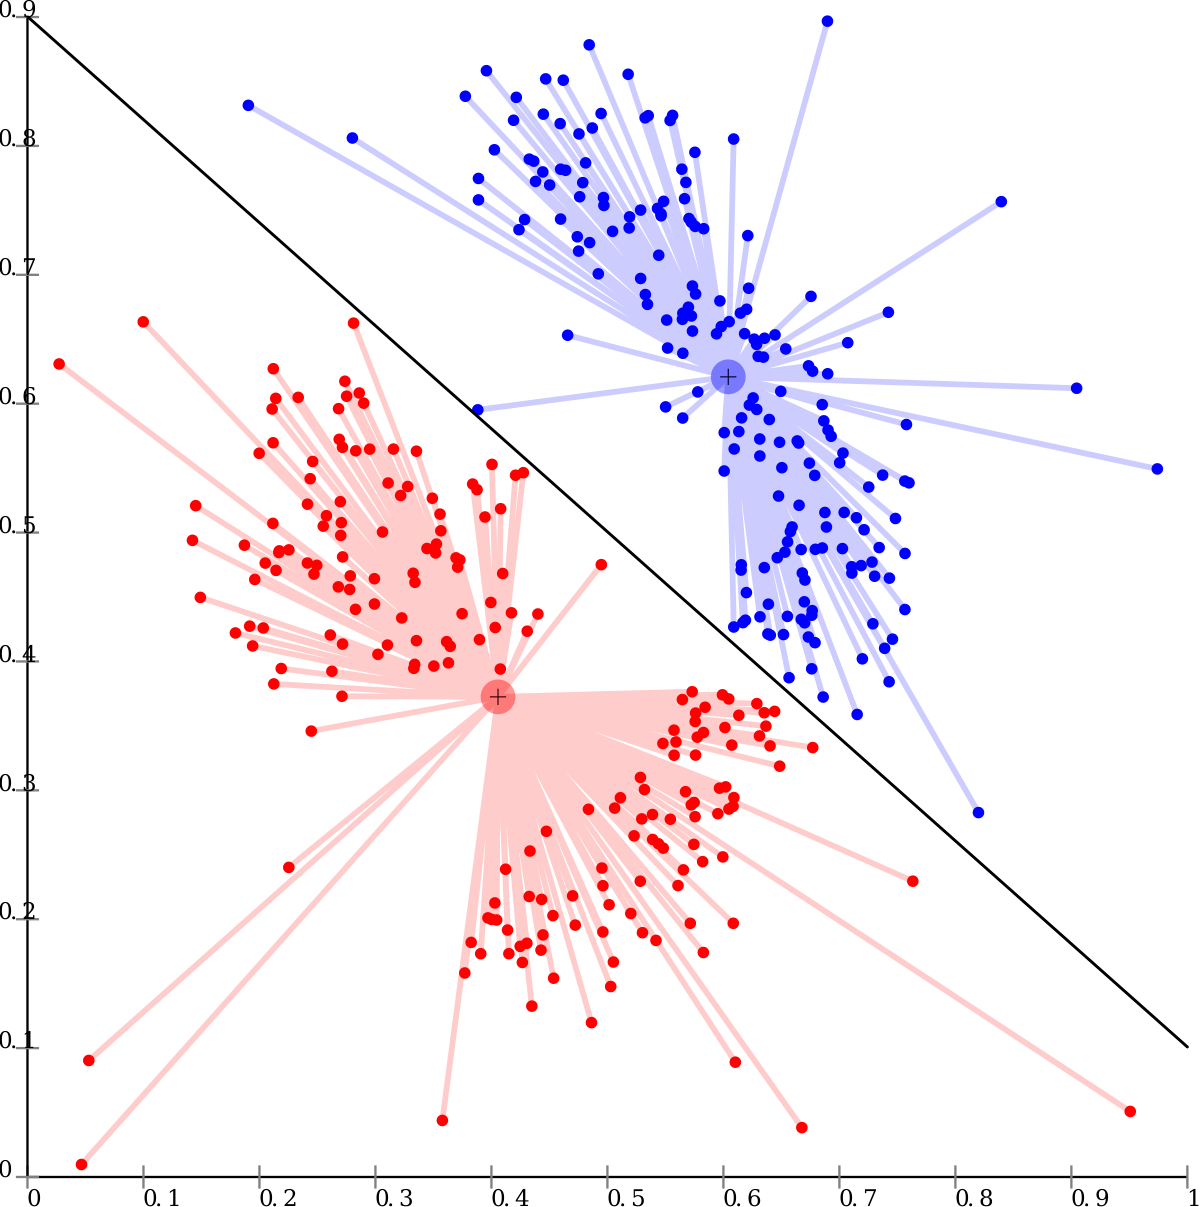
\includegraphics[scale=0.15]{3_6}
    \centering
\end{figure}
\paragraph{Superparamagnetic Clustering}
This method is inspired by statistical mechanics, it does not assume a-priori distributions
for the data, and groups spikes into clusters as a function of a single parameter: the
temperature.\\
It is at the base of the software realized by the group of Rodrigo Quian Quiroga
(University of Leicester, UK) called Wave Clus. This method is implemented as an
iteration (by Monte Carlo method) of a Potts model. The Potts model is a generalization
of the Ising model, where instead of having spins with values \(\pm\frac{1}{2}\), there
are \(q\) different states per particle.
\begin{itemize}
    \item The \(p\)-selected features of a generic \(i\)-th spike are represented by a
          point \(x_i\) in a \(p\)-dimensional phase space. Then, let's define the
          interaction strength between two points \(x_i\) and \(x_j\):
          \begin{align*}
              J_{ij}=
              \begin{cases}
                  \begin{matrix}
                      \frac{1}{K}\exp{\biggl(-\frac{\|x_i-x_j\|^2}{2a^2}\biggr)} &  & \text{if}\,x_i\,\text{is a nearest neighbor of}\,x_j \\
                      0                                                          &  & \text{else}
                  \end{matrix}
              \end{cases}
          \end{align*}
          where \(a\) is the average nearest-neighbor distance and \(K\) is the number
          of nearest neighbors. As a consequence, similar spikes will exhibit a strong
          interaction.
    \item At this point, a random state is assigned to each point \(x_i\) and \(N\)
          Monte Carlo iterations are run for different temperatures \(T\). A point \(x_i\)
          is randomly selected and its state is randomly changed to \(s_{new}\)
          (chosen between 1 and \(q\)). The probability that the nearest neighbors of \(x_i\)
          will change their state to \(s_{new}\) is given by:
          \begin{align*}
              p_{ij}=1-\exp{\biggl(-\frac{J_{ij}}{T}\delta_{s_i,s_j}\biggr)}
          \end{align*}
          This implies that close points will change their status together, forming
          clusters of spikes with similar shape. This observation can be quantified by
          measuring the point-to-point correlation \(\delta_{s_i,s_j}\) and defining
          \(x_i,x_j\) to be members of the same cluster if
          \(\delta_{s_i,s_j}\leq\theta\), for a given threshold \(\theta\).\\
          Moreover:
          \begin{itemize}
              \item \textbf{High temperatures} correspond to a low probability of changing
                    the state \(\Rightarrow\) states change randomly, thus no clusters
                    are formed (paramagnetic phase).
              \item \textbf{Low temperatures} correspond to a high probability of changing
                    to the same state, regardless of the interaction strength \(J_{ij}\)
                    \(\Rightarrow\) all states are changed to the same, thus all spikes
                    belong to the same cluster (ferromagnetic phase).
              \item \textbf{Medium temperatures} correspond to a phase in which only similar
                    spikes will change their state together, forming meaningful clusters
                    (superparamagnetic phase).
          \end{itemize}
\end{itemize}
\begin{figure}[H]
    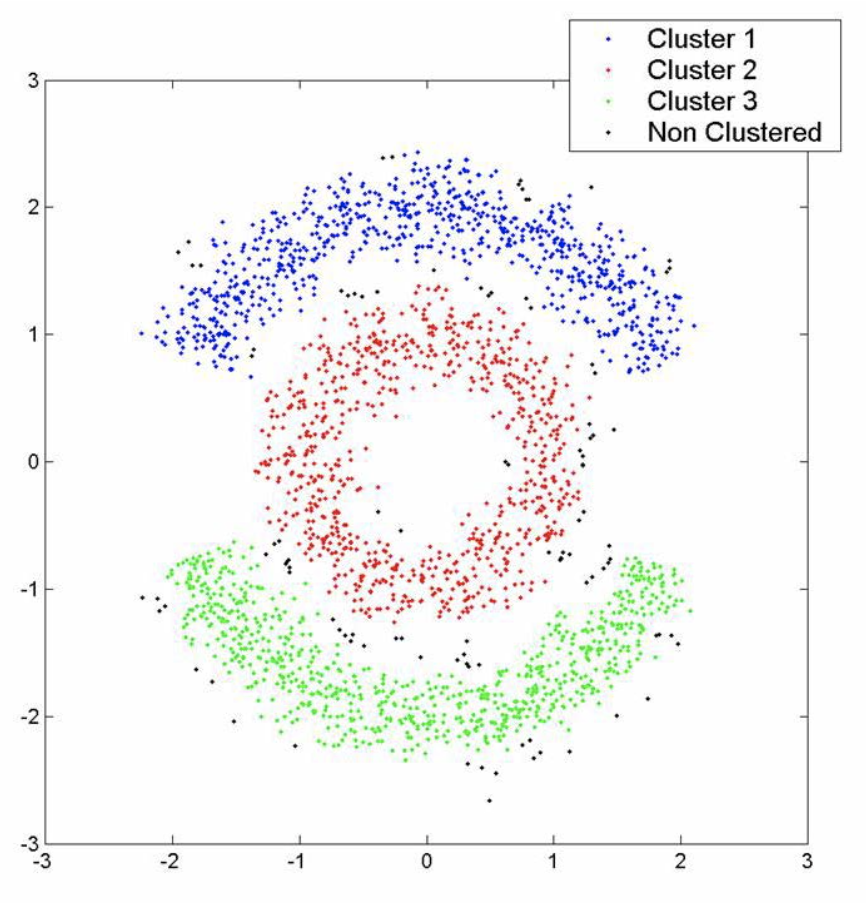
\includegraphics[scale=0.32]{3_7}
    \centering
\end{figure}
In this image some large size clusters corresponding to the optimal sorting can be
observed:
\begin{itemize}
    \item Clusters partially overlap
    \item They have a large variance
    \item The centers fall outside the clusters
    \item The distance between arbitrarily chosen points of the same cluster can
          be much larger than the distance between points in different clusters.
\end{itemize}

\subsection{Miscellanea}
In the following are reported some further remarks and considerations concerning
Spike Sorting.
\subsubsection{Spike Sorting issues}
The main issues when it comes to Spike Sorting are listed below:
\begin{itemize}
    \item \textbf{Electrode Drift:} waveforms of a given neuron vary over
          time and may be assigned to multiple clusters.
    \item \textbf{Tetrodes:} tetrode recordings can be exploited to improve
          spike sorting results, since they allow the visualization of single
          neurons from different positions.
    \item \textbf{Overlapping Spikes:} this phenomenon can be observed when
          two close-by neurons fire in synchrony or with a small delay. Still
          an open issue in Spike Sorting.
    \item \textbf{Bursting Cells:} a burst is the firing of a fast sequence
          of spikes by a neuron. Successive spikes in a burst may have decreasing
          amplitude and may be mistakenly considered as separate clusters.
\end{itemize}
\subsubsection{KiloSort}
Kilosort is a project whose aim is to develop a fully automated, scalable, and accurate
spike sorter, removing the burden of this task from researchers. It belongs to the
template matching class of Spike Sorting algorithms.\\
The main hypothesis of KiloSort is that spatial and temporal shapes of a waveform
provide all the information necessary to assign a given spike to a neuron. This
algorithm exploits template matching in both spike detection and spike clustering,
which are condensed into a single unified model describing the voltage \(V\) of channel
\(i\) at the time instant \(t\):
\begin{align*}
    V(i,t)=\sum_{k=1}^{N_{spike}}A_{\sigma(k)}(i,t-t_k)\cdot x(k) + noise
\end{align*}
with \(A_{\sigma(k)}(i,t-t_k)\) being the spike template for the \(k\)-th neuron
and \(x(k)\) the amplitude of the spike emitted by the \(k\)-th neuron. Hence, it
basically omits spike detection and PCA (both of these steps may discard potentially
useful information) and instead combines the identification of template waveforms and
associated spike times.
\subsubsection{Performance evaluation}
Different Spike Sorting methods can be compared by testing them on simultaneous
extracellular and intracellular recordings datasets, in a similar fashion with respect
to Spike Detection. Often, simulated datasets are used, where the identity of each
spike is known: it is important to create datasets that mimic as accurately as possible
the characteristics of real recordings in terms of noise distribution, spike features,
and so on.\\
The SpikeForest project aims at benchmarking and testing the finest and most recent
Spike Sorting algorithms.

\newpage

\section{Spike Analysis}
\graphicspath{ {./images/4/} }
\subsection{Introduction}
As already stated in the previous chapters, it is well-known that in general the electrophysiological
signal (acquired from a single electrode) is characterized by 2 distinct patterns:
\begin{itemize}
    \item \textbf{Spike:} a single over-threshold signal representing the activity of one or
          more neurons (typically a so-called unit or channel).
    \item \textbf{Burst:} a sequence of highly packed spikes often occurring simultaneously on
          several channels and giving rise to a phenomenon known as network burst.
\end{itemize}
\begin{figure}[H]
    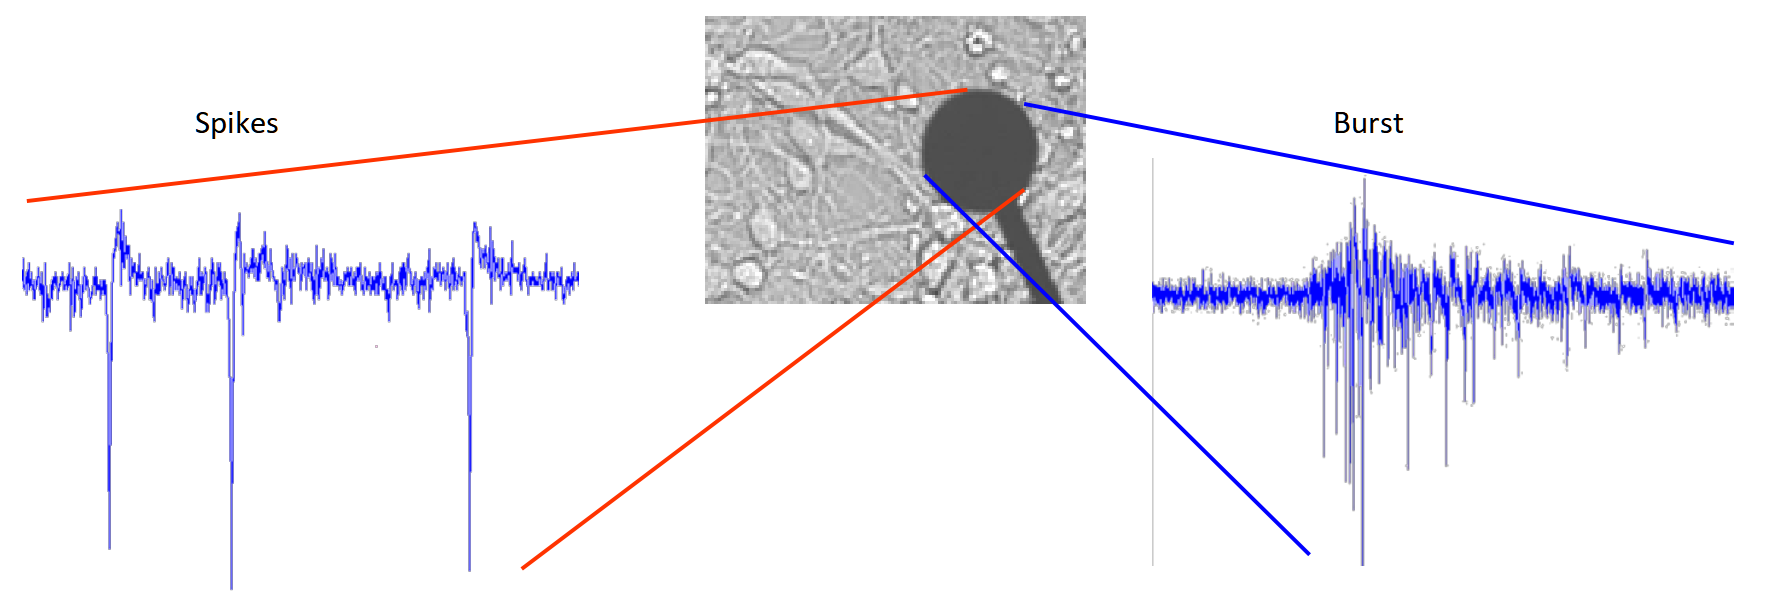
\includegraphics[scale=0.4]{4_1}
    \centering
\end{figure}


\subsection{Data visualization tools}
The first preliminary steps of Spike Analysis consist in taking a look at the raw data, then
deriving the spike train for each channel and visualize it. Therefore, it might be useful to define
a set of proper plots and metrics for data visualization.
\subsubsection{Raw data multi-channel plot}
The following plot shows the activity - i.e. voltage - recorded by 8 distinct electrodes as a
function of time.
\begin{figure}[H]
    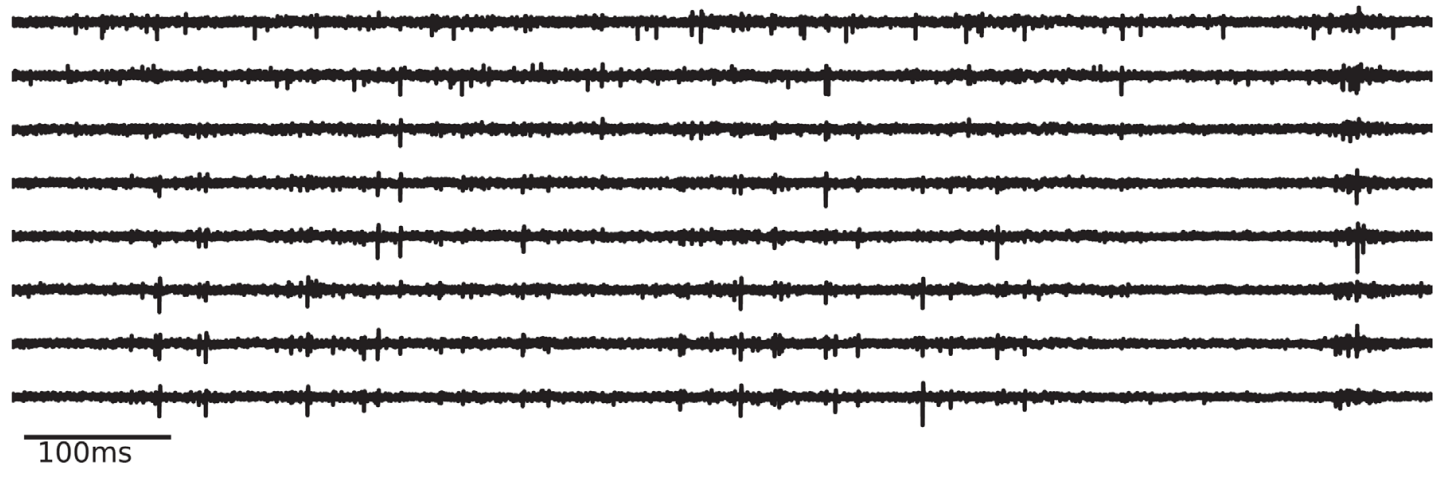
\includegraphics[scale=0.4]{4_2}
    \centering
\end{figure}
\subsubsection{Raster Plot}
The Raster Plot (also known as Spike Raster) is done after Spike Sorting and it allows to visualize
at the same time the spike trains coming from multple recording electrodes on the same time axis.
It is common to observe consistent activation patterns across channels, as neurons influence each
other.
\begin{figure}[H]
    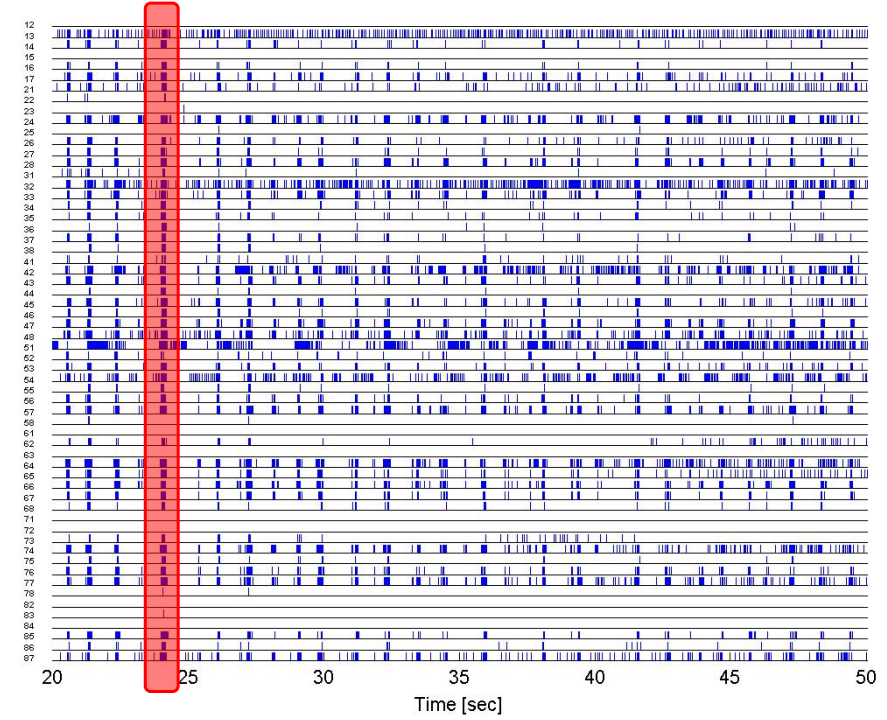
\includegraphics[scale=0.75]{4_3}
    \centering
\end{figure}
\subsubsection{Task-Related Raster Plot}
The Task-Related (or Stimulus-Related) Raster Plot is similar to the ordinary Raster Plot, even if it
has a quite different meaning: the multiple lines do not represent channels, but portions of the
recording coming from just one channel. The signal portions are divided according to the execution of
a task or the receiving of a stimulus.
\begin{figure}[H]
    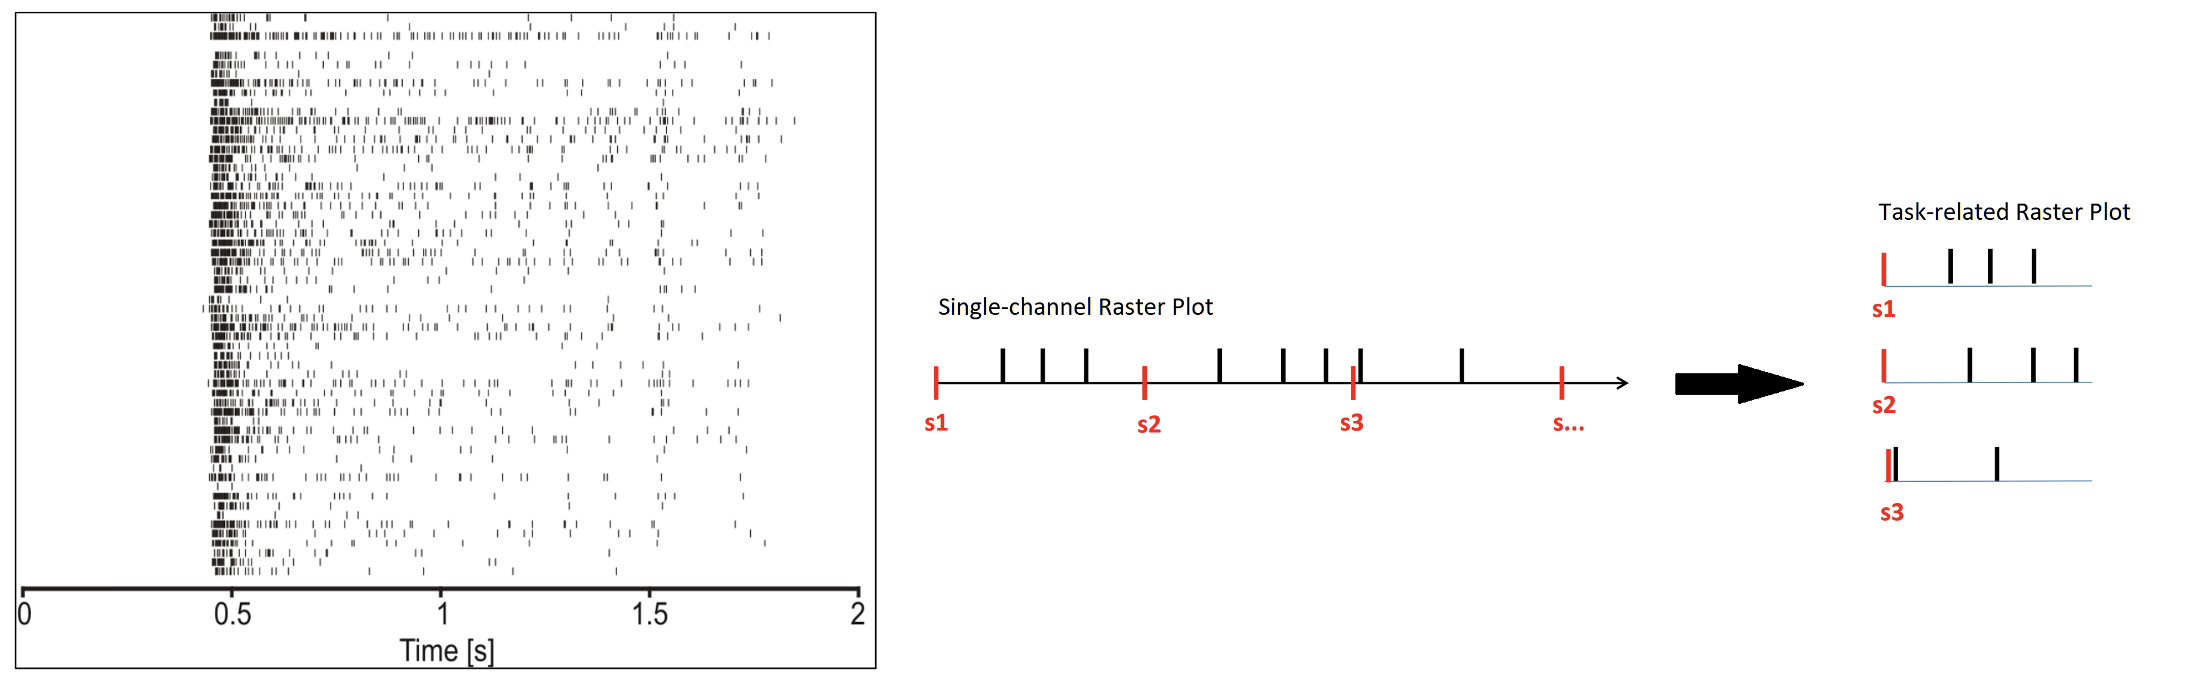
\includegraphics[scale=0.4]{4_4}
    \centering
\end{figure}
\subsubsection{High-Density Data Raster Plot}
This is once again a type of Raster Plot. Data comes from several channels and they cover a relatively
large span of time. As a consequence, it is almost impossible to distinguish single spikes by eye,
thus this high-density plot is usually inspected by looking at the shaded regions, as they exhibit a
higher concentration of fired spikes, implying a greater activity.
\begin{figure}[H]
    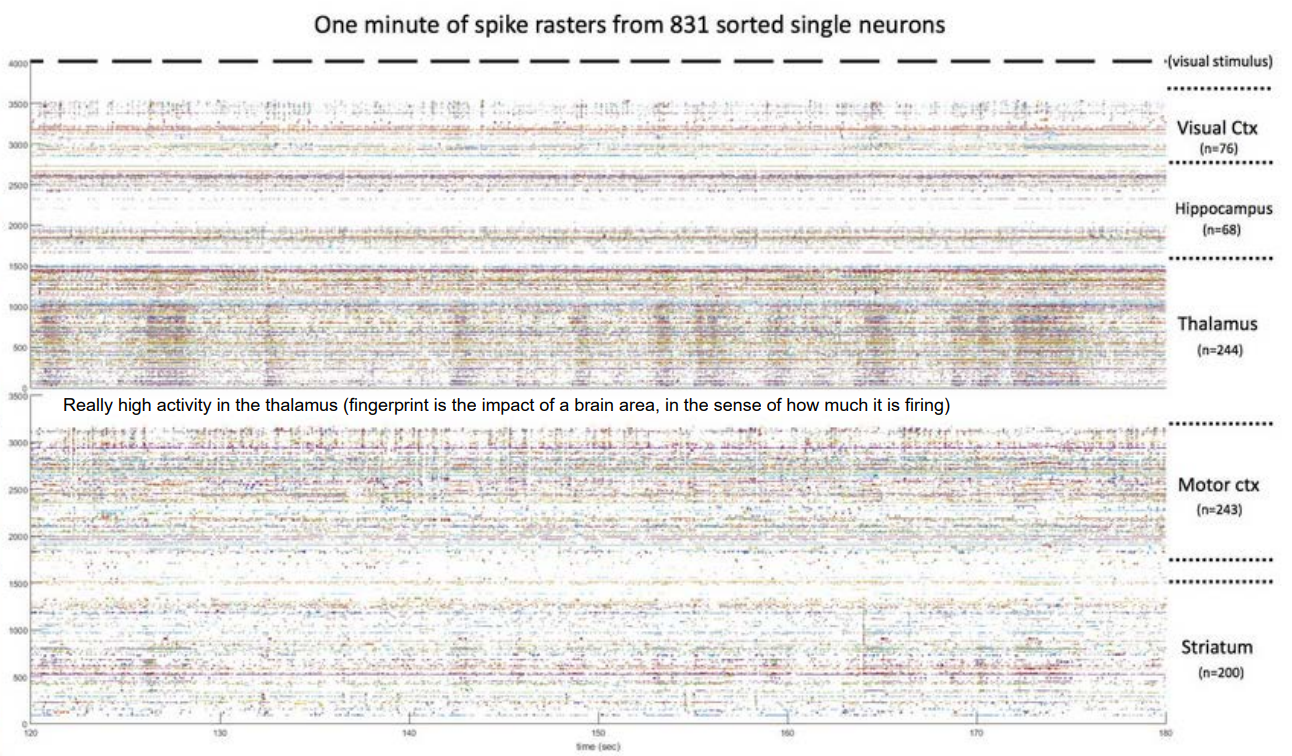
\includegraphics[scale=0.6]{4_5}
    \centering
\end{figure}
\subsubsection{Spike Count and Firing Rate metrics}
\paragraph{Spike Count}
This metric is obtained by dividing the time axis into equal bins \(\Delta{t}=[t_a,t_b]\) and just
counting the number of spikes \(N_{ab}\) occurring in each bin.
Then, an histogram showing the Spike Count can be plotted.
\paragraph{Instantaneous Firing Rate}
By simply taking the Spike Count and dividing it by the bin size, the Instantaneous Firing Rate (IFR)
can be derived.
\begin{align*}
    IFR=r(t)=\frac{N_{ab}(t)}{\Delta{t}}
\end{align*}
The IFR is measured in spikes per second.
\paragraph{Spike Density Function}
The Spike Density Function (SDF) is obtained by associating a proper distribution (typically Gaussian)
to each single spike, then the SDF is derived by summing up the various individual distributions.
\begin{figure}[H]
    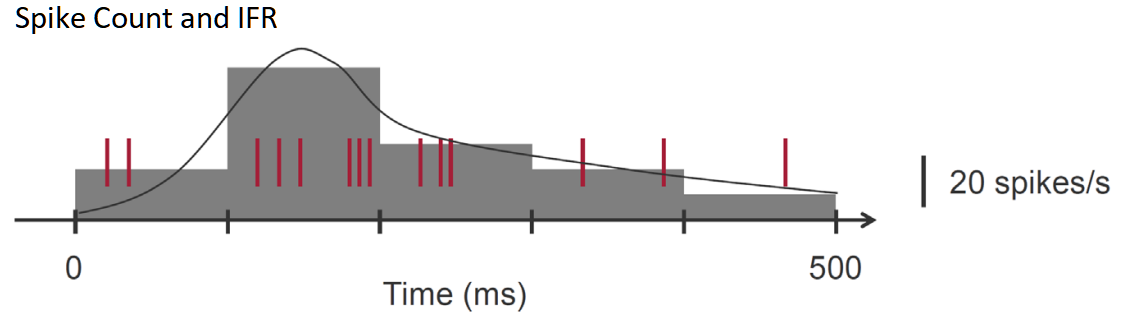
\includegraphics[scale=0.6]{4_6}
    \centering
\end{figure}
\paragraph{Array-Wide Firing Rate}
The Array-Wide Firing Rate (AWFR), often called Average Firing Rate (AFR), it is a sort of
IFR by taking into account the whole network - i.e. all the recorded channles, not just a single one.
This metric is often employed in neuropharmacology, in order to assess the time of response of a drug.\\
By setting the number of channels - i.e. the number of electrodes - to \(M\), the AFR is defined as:
\begin{align*}
    AWFR=awfr(t)=mean(IFR)=\frac{1}{M}\sum_{j=1}^{M}r_{j}(t)
\end{align*}
\paragraph{Mean Firing Rate}
The Mean Firing Rate (MFR) represents a single numerical metric of the activity of neurons for the
entire network (\(M\) channels). It is expressed as
\begin{align*}
    MFR=\frac{1}{T}\sum_{j=1}^{M}N_j
\end{align*}
where \(T\) is the considered time window (somehow corresponding to the previously seen \(\Delta{t}\)),
while \(N_j\) is the number of spikes recorded in the \(T\) interval for the \(j\)-th electrode.\\
Notice once again that both IFR and AWFR are functions of time, continuous in the time-domain, while
MFR is a single value giving information on the average degree of activation of the whole neural
network in a determined time interval.\\
The following plot illustrates the Mean Firing Rate, indicating the average neural activity, at
different concentrations of a brain inhibitor drug.
\begin{figure}[H]
    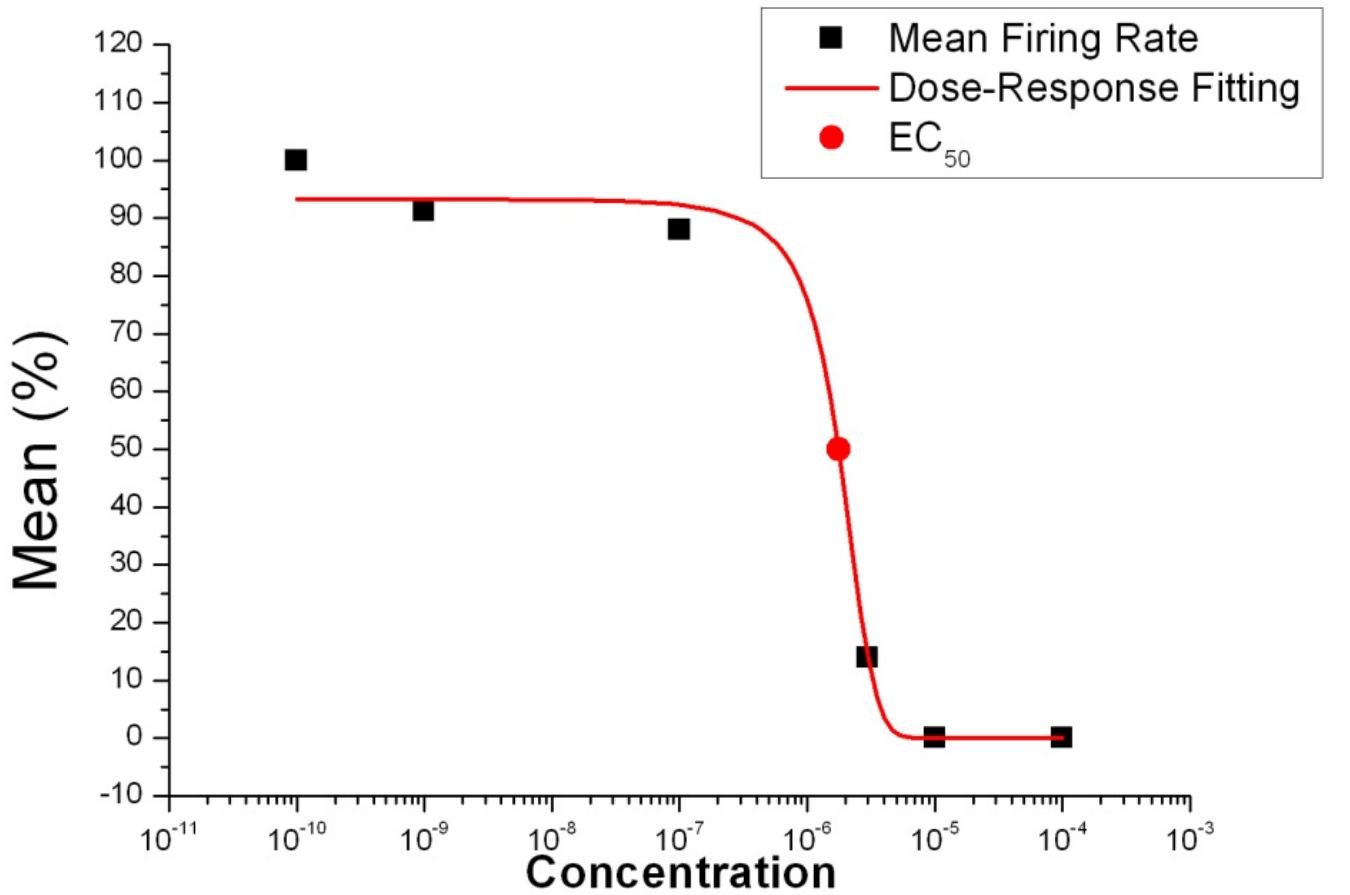
\includegraphics[scale=0.35]{4_7}
    \centering
\end{figure}
\subsubsection{Inter Spike Interval}
\paragraph{Inter Spike Interval}
The Inter Spike Interval (ISI) is the interval between two consecutive spikes. It is used to compute
the Inter Spike Interval Histogram (ISIH), an index of the probability that a spike is fired
a certain time \(\tau\) after a reference spike.
Given \(N\) spikes, the ISIH metric is computed as shown below:
\begin{align*}
    ISIH(\tau)=\frac{1}{N-1}\sum_{s=1}^{N-1}\delta{(t_{s+1}-t_{s}-\tau)}
\end{align*}
An histogram as the following one is often employed to visualize the metric.
\begin{figure}[H]
    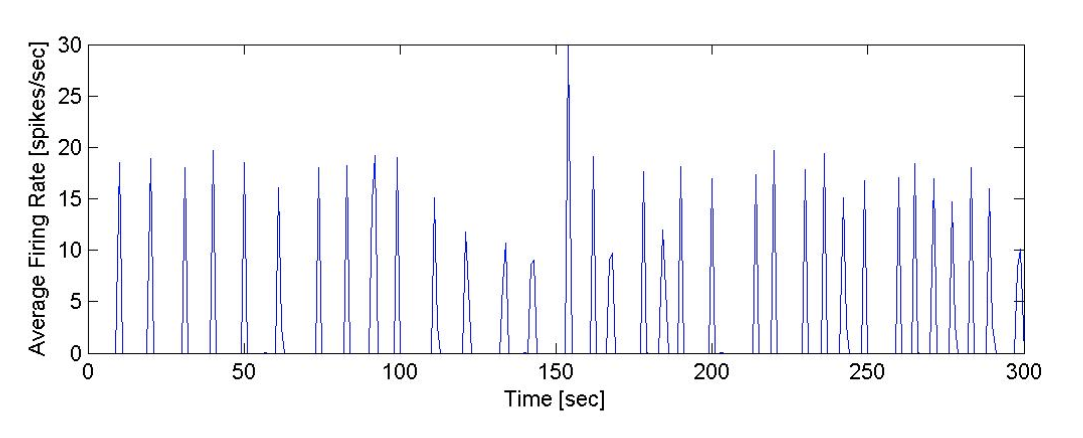
\includegraphics[scale=0.5]{4_8}
    \centering
\end{figure}
Notice that it is common to have a higher probability close to the reference spike, while it tends to
decrease as the Inter Spike Interval grows. If the spike train is made of packed spikes alternating
to empty intervals, then the histogram will display 2 distinct peaks: one for the high frequency
component and one for the low frequency component.
\paragraph{Joint Inter Spike Interval}
The Joint Inter Spike Interval (JISI) is derived from the ISI and it is useful to evaluate the
relationship between pre-ISI and post-ISI intervals, for any spike of the train.
The probability JISIH for \(N\) spikes is computed as:
\begin{align*}
    JISIH(\tau_{post},\tau_{pre})=\frac{1}{N-2}\sum_{s=2}^{N-1}\delta{(t_{s+1}-t_{s}-\tau_{post})}\ast \delta{(t_s-t_{s-1}-\tau_{pre})}
\end{align*}
In this case the plot becomes tridimensional, however it can be displayed in 2D by using
colormaps.
\begin{figure}[H]
    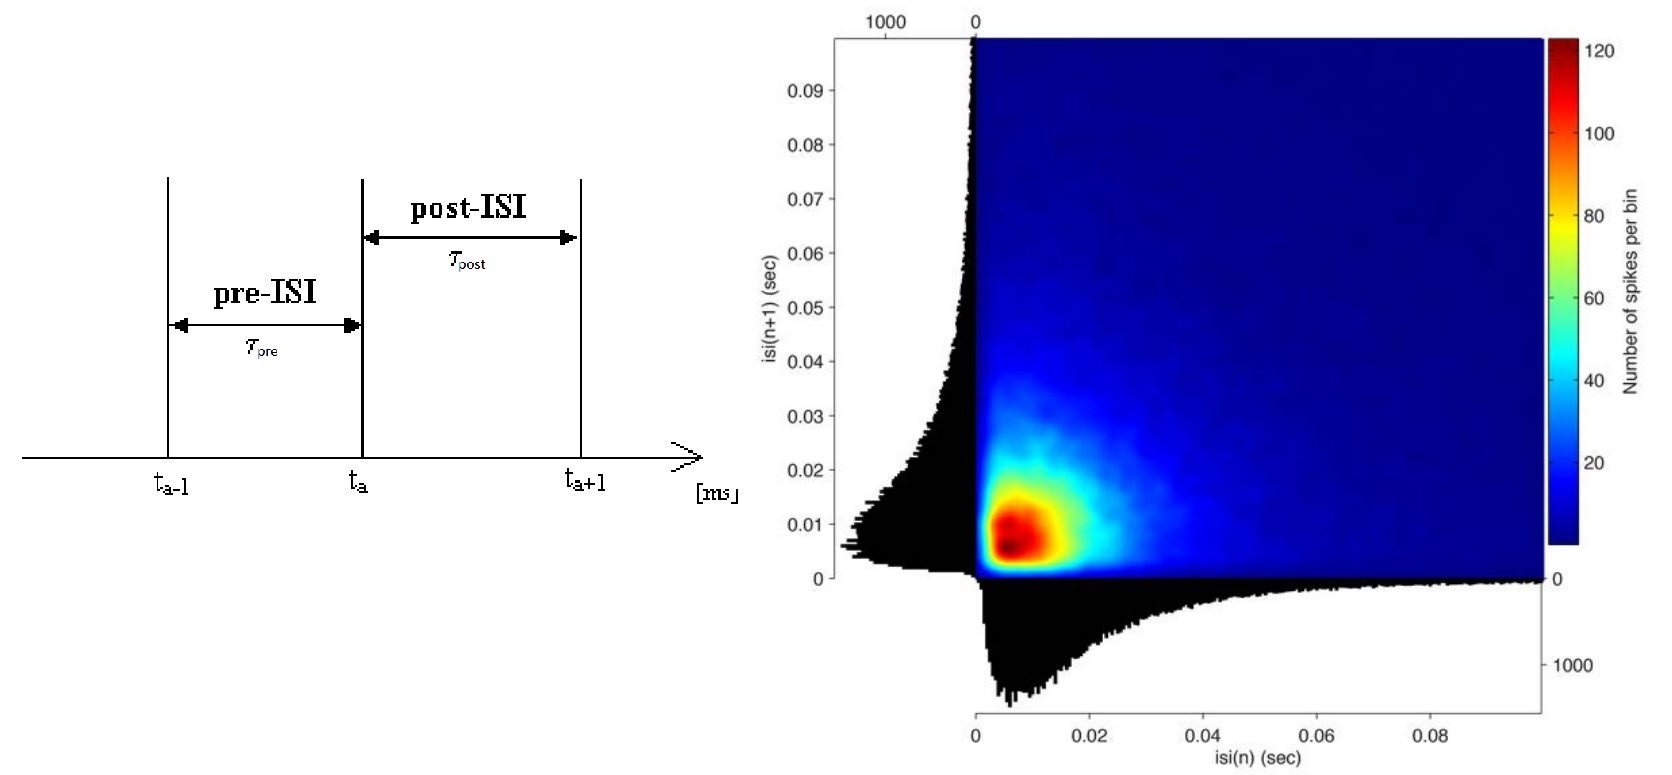
\includegraphics[scale=0.45]{4_9}
    \centering
\end{figure}
\paragraph{Cross Inter Spike Interval}
The Cross Inter Spike Interval (CISI) works in a fashion similar to JISI, but it analyzes the
dependance between spikes of two different trains. The probability CISIH is given by:
\begin{align*}
    CISIH(\tau_{post},\tau_{cross})=\frac{1}{N-2}\sum_{a=1}^{N_a-1}\delta{(t_{a+1}-t_{a}-\tau_{post})}\ast \delta{(t_a-t_b-\tau_{cross})}
\end{align*}
\begin{figure}[H]
    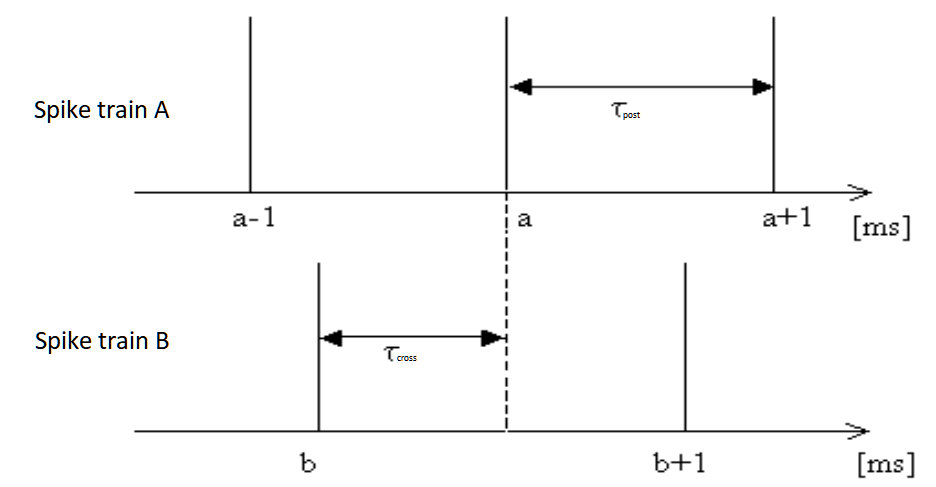
\includegraphics[scale=0.5]{4_10}
    \centering
\end{figure}

\subsection{Spike Generation Modelling}
Several neurons exhibit a considerable degree of variability in their firing
sequence, especially in \textit{in vivo} recordings. Therefore, a class of irregual
spike trains model can be defined after these 3 assumptions:
\begin{enumerate}
    \item Every spike is generated randomly.
    \item Every spike is independent of other spikes.
    \item Every spike has a uniform probability of occurrence in time.
\end{enumerate}
A simple model exploiting the Poisson distribution can be built and it is comparable
to actual spike trains, due to the independence between the time of occurrence of
neighbouring spikes. However, real spike trains tend to have inter spike intervals
(ISI) dependent on the preceding spike intervals.
In general, a Poisson spike sequence is well-suited at describing tonic firing
neurons.
\subsubsection{Derivation of the Homogenous Poisson Process}
Firstly, let's set an assumption: the firing rate - i.e. the average number
of fired spikes in a unit of time - is assumed to be constant, thus
\(r(t)=r=\frac{n}{T}\), where \(n\) is the overall number of observed spikes
and \(T\) is the total observation period.\\
Now, let's divide the observation period \(T\) in a number \(M\) of bins having
equal length, such that \(M=\frac{T}{\Delta{t}}\). Let's consider a
number of bins \(M\) such that every bin contains 1 or 0 spikes. Therefore,
the probability of finding 1 spike in a time interval \(\Delta{t}\) (coincident
with 1 bin) is:
\begin{align*}
    P\{\text{1 spike in}\,\Delta{t}\}=P_{\Delta{t}}[1]
    =\frac{\text{Number of spikes in}\,T}{\text{Number of bins}\,\Delta{t}}
    =\frac{r\cdot{T}}{M}
    =r\cdot\frac{T}{M}
    =r\cdot{\Delta{t}}
\end{align*}
Let's call \(P\{n\,\text{spikes in}\,T\}=P_T[n]\) the probability of finding \(n\)
spikes in the observation period \(T\). It is the product of three distinct factors:
\begin{itemize}
    \item \(P\{\text{Generating}\,n\,\text{spikes within}\,n\,\text{bins}\}
          =\bigl(r\cdot{\Delta{t}}\bigr)^n\)
    \item \(P\{\text{Not generating any spike in the remaining bins}\}
          =\bigl(1-r\cdot{\Delta{t}}\bigr)^{M-n}\)
    \item The number of combinations to put \(n\) spikes in \(M\) bins
          \(\Rightarrow\binom{M}{n}=\frac{M!}{(M-n)!\cdot{n!}}\)
\end{itemize}
Finally, the Poisson model can be written as follow, by recalling the binomial formula:
\begin{align*}
    P=\binom{M}{n}\cdot{p^n}\cdot{q^{M-n}}
\end{align*}
At this point, let's compute the product and try to rearrange it:
\begin{align*}
    P_T[n]=P\{n\,\text{spikes in}\,T\}
     & =\lim_{\Delta{t}\to{0}}\binom{M}{n}\cdot{p^n}\cdot{q^{M-n}}                                                                         \\
     & =\lim_{\Delta{t}\to{0}}\frac{M!}{(M-n)!\cdot{n!}}\cdot{\bigl(r\cdot{\Delta{t}}\bigr)^n}\cdot{\bigl(1-r\cdot{\Delta{t}}\bigr)^{M-n}}
\end{align*}
Let's set \(\epsilon=-r\cdot{\Delta{t}}\Rightarrow \Delta{t}=-\frac{\epsilon}{r}\)
and \(M=\frac{T}{\Delta{t}}=\frac{T}{-\frac{\epsilon}{r}}=-\frac{r\cdot{T}}{\epsilon}\).
For \(\Delta{t}\to{0}\), the number of bins \(M\) becomes larger and larger,
thus \(\bigl(M-n\bigr)\sim{M}=\frac{T}{\Delta{t}}\), leading to:
\begin{align*}
    \lim_{\Delta{t}\to{0}}\bigl(1-r\cdot{\Delta{t}}\bigr)^{M-n}
    \sim\lim_{\Delta{t}\to{0}}\bigl(1-r\cdot{\Delta{t}}\bigr)^M
     & =\lim_{\epsilon\to{0}}\bigl(1+\epsilon\bigr)^M
    =\lim_{\epsilon\to{0}}\bigl(1+\epsilon\bigr)^{-\frac{r\cdot{T}}{\epsilon}}                      \\
     & =\lim_{\epsilon\to{0}}\biggl[\bigl(1+\epsilon\bigr)^{\frac{1}{\epsilon}}\biggr]^{-r\cdot{T}}
    =e^{-r\cdot{T}}
\end{align*}
Let's now consider the binomial coefficient part:
\begin{align*}
    \frac{M!}{(M-n)!\cdot{n!}}
    \sim\frac{M^n}{n!}
    =\frac{\bigl(\frac{T}{\Delta{t}}\bigr)^n}{n!}
    =\frac{T^n}{\Delta{t}^n\cdot{n!}}
\end{align*}
Therefore:
\begin{align*}
    P_T[n]
     & =\lim_{\Delta{t}\to{0}}\frac{M!}{(M-n)!\cdot{n!}}\cdot{\bigl(r\cdot{\Delta{t}}\bigr)^n}\cdot{\bigl(1-r\cdot{\Delta{t}}\bigr)^{M-n}} \\
     & =\frac{T^n}{\Delta{t}^n\cdot{n!}}\cdot{\bigl(r\cdot{\Delta{t}}\bigr)^n}\cdot{e^{-r\cdot{T}}}                                        \\
     & =\frac{T^n}{\cancel{\Delta{t}^n}\cdot{n!}}\cdot{r^n\cdot{\cancel{\Delta{t}^n}}}\cdot{e^{-r\cdot{T}}}                                \\
     & =\frac{\bigl(rT\bigr)^n}{n!}\cdot{e^{-rT}}
\end{align*}
Let's now consider two subsequent time instants \(t_0\) and \(t_0+\tau\), then compute
the following probabilities:
\begin{align*}
    P\{0\,\text{spikes in}\,[t_0,t_0+\tau]\}
    = \frac{\bigl(rT\bigr)^n}{n!}\cdot{e^{-rT}}
    = e^{-rT}
    \quad\quad\quad\text{as \(n=0\)}
\end{align*}
\begin{align*}
    P\{1\,\text{spikes in}\,[t_0,t_0+\tau]\}
    = \frac{\bigl(rT\bigr)^n}{n!}\cdot{e^{-rT}}
    = 1-e^{-rT}
    \quad\quad\quad\text{as \(n=1\)}
\end{align*}
Therefore, the cumulative distribution is 0 for \(\tau=0\) and it increases
monotonically for \(\tau\to{+\infty}\). This means that, after a spiking event,
the longer it is waited, the bigger is the chance for another spike to occur.
At this point, the probability density function describing the waiting times to
have a new spiking event can be expressed as the derivative of the cumulative
distribution:
\begin{align*}
    pdf(\tau)
    =p(\tau)
    =\frac{d}{dt}\bigl(1-e^{-r\tau}\bigr)
    =-(-r)\cdot{e^{-r\tau}}
    =r\cdot{e^{-r\tau}}
\end{align*}
Notice that this last expression represent the distribution of the Inter Spike
Interval (ISI) histogram of a Poisson distribution, with \(\frac{1}{r}\) being
the mean delay between two consecutive events.
Another point to highlight is that the choice of \(t_0\) does not affect the chance
to generate a spike after a time interval \(\tau\).
By chanching the involved variables, the probability density function of a
Poisson distribution, intended as the chance to generate a spike event after a time
\(t\) from a reference spike, is given by
\begin{align*}
    pdf(t)
    =p(t)
    =\frac{1}{\overline{t}}e^{-\frac{t}{\overline{t}}}
\end{align*}
with \(t=\tau\) and \(\frac{1}{\overline{t}}=r=AFR\).\\
In general, the function \(p(t)\) - i.e. the ISI histogram - is obtained
experimentally by binning consecutive inter spike intervals.

\subsubsection{Metrics related to ISI histograms}
\paragraph{Coefficient of Variation}
It is the simplest index to measure the variability of the ISI distribution. The
coefficient of variation \(C_v\) is a dimensionless number computed as the
s.t.d. of the ISI distribution normalized by the mean interspike interval:
\begin{align*}
    C_v=\frac{\sigma_t}{\overline{t}}
\end{align*}
Notice that if the ISI distribution s.t.d. is equal to the mean ISI, then
\(C_v=1\), as in the case of a Poisson distribution. On the other hand,
\(C_v=0\) for a sequence of perfectly regular intervals.

\paragraph{Local Variation}
The previously introduced coefficient of variation \(C_v\) represents the global
variability of an entire ISI sequence, thus it is sensitive to firing rate
fluctuations. Sometimes this might not be enough to discriminate between really
different ISI sequences, as long as they have an equal average firing rate. Hence,
the local variation coefficient \(L_v\) is to be introduced as follow:
\begin{align*}
    L_v
    =\frac{3}{n-1}\sum_{i=1}^{n-1}\biggl(\frac{I_{i}-I_{i+1}}{I_{i}+I_{i+1}}\biggr)^2
    =\frac{3}{n-1}\sum_{i=1}^{n-1}\biggl(1-\frac{4I_{i}I_{i+1}}{(I_{i}+I_{i+1})^2}\biggr)
\end{align*}
This metric is capable to detect also the Instantaneous variability of inter spike
intervals. In other words, the local variation takes into account also the
temporal localization of spikes with respect to one another, not jsut their
average distribution.\\
The following picture is especially useful to emphasize the difference between
\(C_v\) and \(L_v\). The presented spike trains are significantly different from
one another, but their overall distribution is similar. As a result, the
coefficient of variation \(C_v\) is the same, while the local variation \(L_v\)
changes according to the relative distribution of spikes.
\begin{figure}[H]
    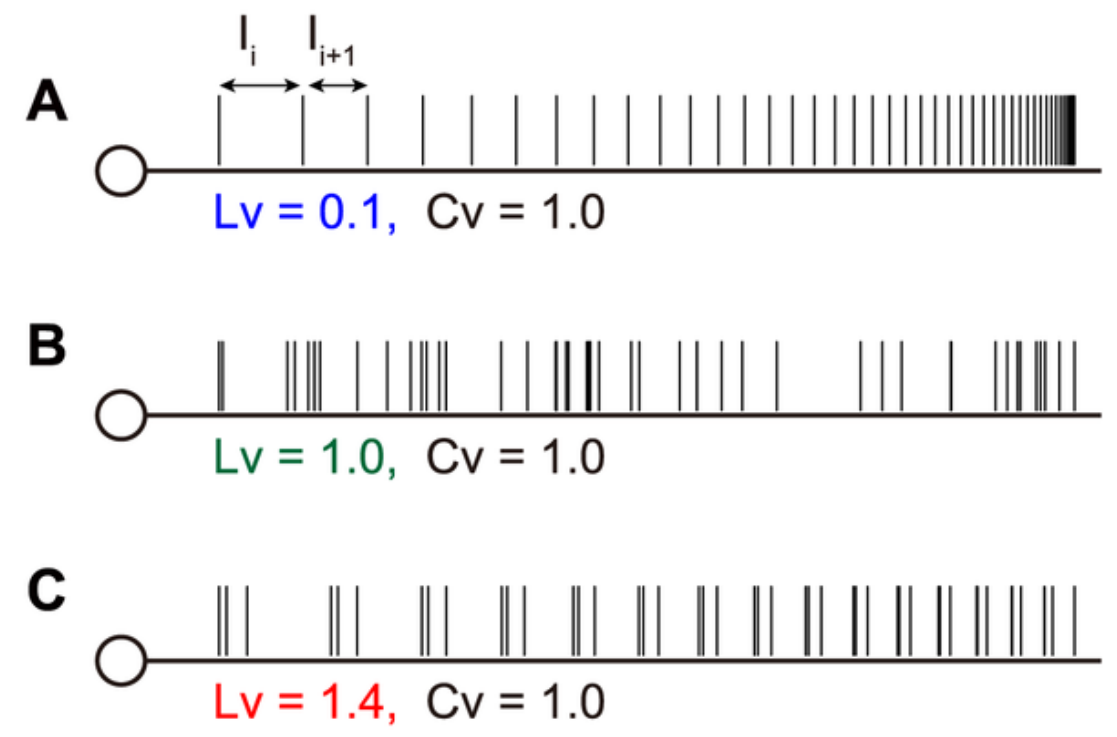
\includegraphics[scale=0.35]{4_11}
    \centering
\end{figure}

\paragraph{LvR}
This metric known as \(L_{v}R\) represents an enhancement with respect to the widely
employed local variation \(L_v\), as a matter of fact it exhibits an enhanced
invariance w.r.t. firing rate fluctuations. It is defined by the expression below:
\begin{align*}
    L_{v}R
    =\frac{3}{n-1}\sum_{i=1}^{n-1}\biggl(1-\frac{4I_{i}I_{i+1}}{(I_{i}+I_{i+1})^2}\biggr)\biggl(1+\frac{4R}{I_{i}+I_{i+1}}\biggr)
\end{align*}
where \(R\) is the refractoriness constant.
This coefficient allows to distinguish among 3 main classes of spike generation,
according to the displacement of spikes with respect to one another:
\begin{itemize}
    \item \(\mathbf{L_{v}R\sim0.5}\Rightarrow\,\)regular pattern
    \item \(\mathbf{L_{v}R\sim1}\Rightarrow\,\)random pattern
    \item \(\mathbf{L_{v}R\sim1.5}\Rightarrow\,\)bursty pattern
\end{itemize}
The image reported in the following shows the previously mentioned 3 spike generation
patterns, in this case employed to identify specific cortical areas.
\begin{figure}[H]
    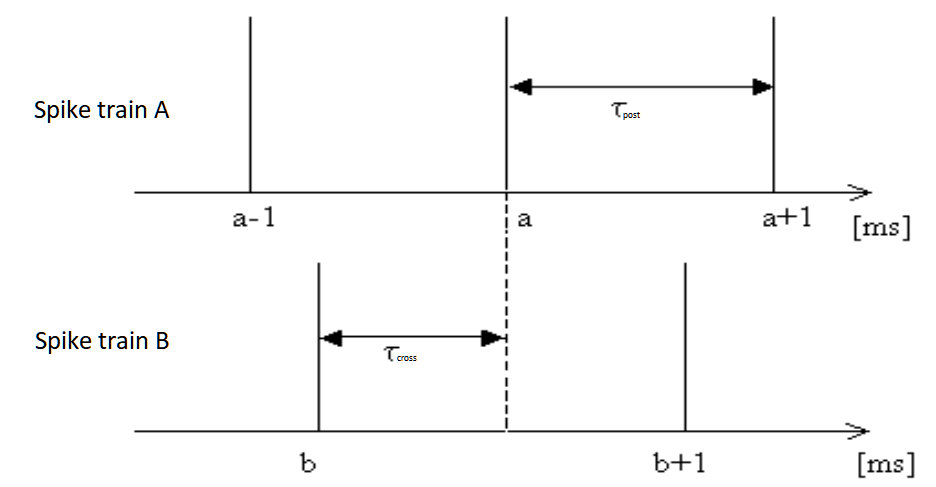
\includegraphics[scale=0.75]{4_12}
    \centering
\end{figure}
\newpage

\section{Burst Detection}
\graphicspath{ {./images/5/} }
\subsection{Introduction}
The electrophysiological signal (acquired from a single electrode) is generally
characterized by two distinct patterns:
\begin{itemize}
    \item \textbf{Spike:} a single over-threshold signal representing the
    electrical activity of a source.
    \item \textbf{Burst:} a sequence of highly packed spikes, often occurring on
    multiple channels at the same time (network burst).
\end{itemize}
Bursting can be defined as a dynamic state with neurons firing discrete groups of
spikes in a repeated manner. A burst is generally followed by a period of quiescence
period. If 2 spikes form a burst are said to be a doublet, 3 are called a triplet,
and so on.
\begin{figure}[H]
    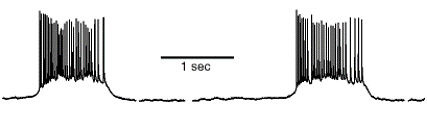
\includegraphics[scale=1.2]{5_1}
    \centering
\end{figure}
Neural bursting plays a key role in communication between neurons, in particular
burst nerons are crucial in mottor pattern generation and synchronization.
Basically all neurons can burst if pharmacologically stimulated, however
it is common to observe autonomous bursting activity, especially in the following
types of neurons:
\begin{itemize}
    \item \textbf{IB:} intrinsically bursting neurons, mostly pyramidal neurons in
    layer 5.
    \item \textbf{CH:} chattering neurons, pyramidal neurons in layers 2, 3, and 4.
    \item \textbf{Interneurons:} present in the cortex.
    \item \textbf{LTB:} low-threshold bursters, they fire high-frequency bursts in
    response to injected pulses of current. Localized in the hippocampus.
    \item \textbf{HTB:} high-threshold bursters fire bursts only in response to
    strong long pulses of current. Localized in the hippocampus.
\end{itemize}
\paragraph{Why do bursts naturally occur?}
There are several hypoteses aiming to explain the importance of bursting activity in
neural computation.
\begin{itemize}
    \item \textbf{Bursts are more reliable than single spikes} in evoking responses in
    postsynaptic cells.
    \item \textbf{Bursts overcome synaptic transmission failure}, it has been shown
    that a synaptic release is more likely to occur in response to a bombardment
    of spikes (instead of a single spike).
    \item \textbf{Bursts evoke long-term potentiation}, thus affecting synaptic
    plasticity in a much greater way than single spikes.
    \item \textbf{Bursts have a higher sinal-to-noise ratio} than single spikes, as
    the generation of bursts requires a higher threshold.
    \item \textbf{Bursts encode different features} of sensory input than single
    spikes.
    \item \textbf{Bursts have more informational content} than single spikes, in
    particular when analyzed as unitary events. This information might be encoded
    into the burst duration or in the precise temporal structure of inter spike
    intervals within a burst. 
\end{itemize}
To summarize, it is important to point out that bursts are all-or-none events,
whereas single spikes may be noise.\\
Despite everything, the term burst lack a formal definition, but it is generally employed
to indicate a recording period during which the spiking frequency is especially high,
alternating with periods exhibiting a low spiking frequency (quiescence periods). Therefore,
it can be stated that a burst is characterized by \textbf{small inter spike intervals} and a
\textbf{certain number of spikes}.
\begin{figure}[H]
    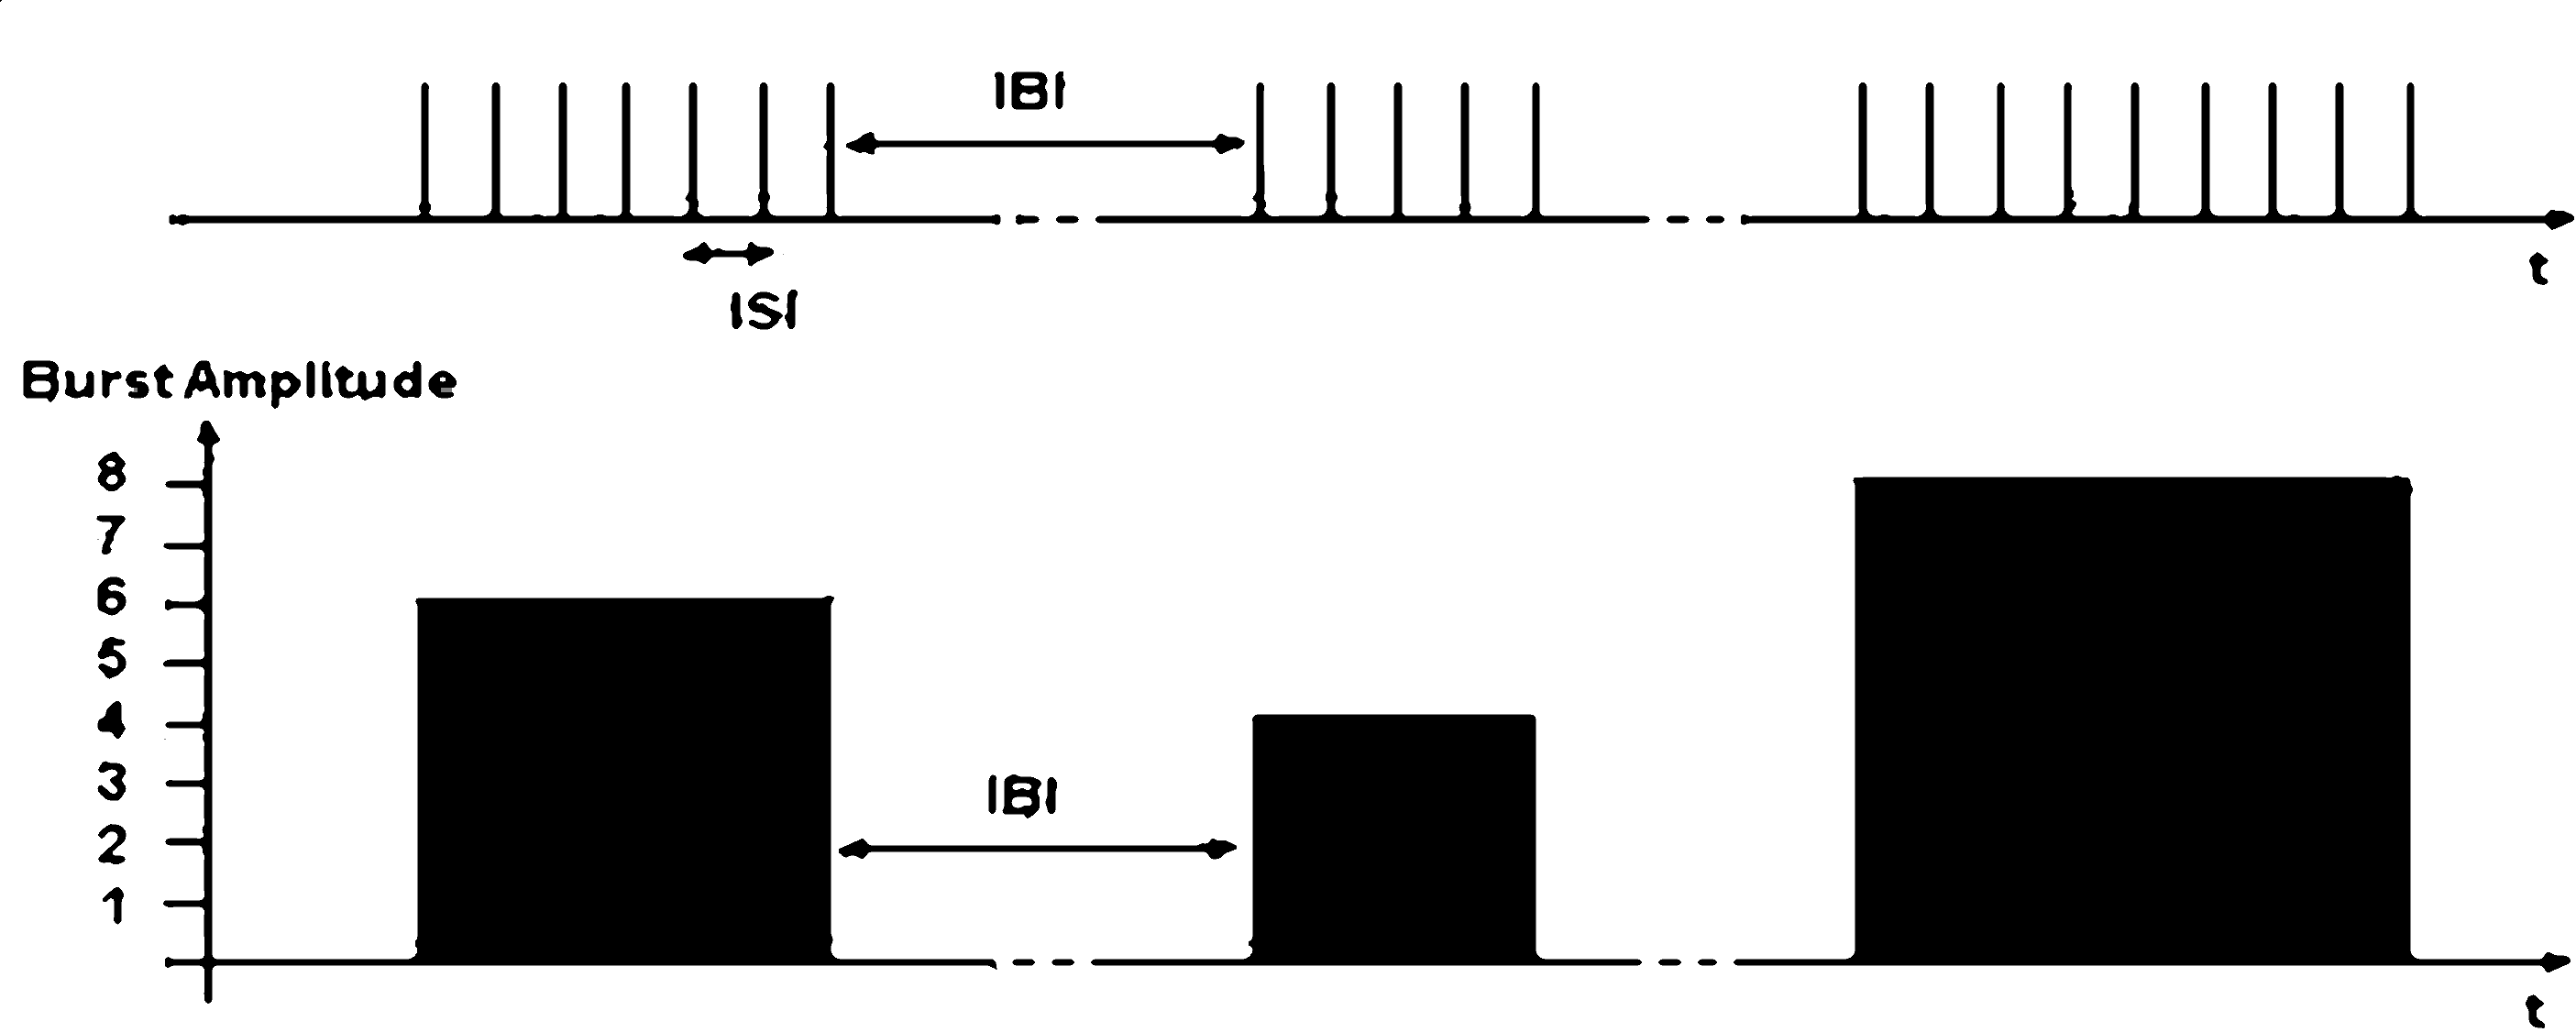
\includegraphics[scale=0.25]{5_2}
    \centering
\end{figure}
From a mathematical point of view, a burst can be defined by some properties, such as:
\begin{itemize}
    \item \(t_b\): the starting time of the burst.
    \item \(T_b\): the burst duration.
    \item \(A_b\): the burst amplitude, related to the spike frequency within the burst.
\end{itemize}
The amplitude of a burst is computed as shown below:
\begin{align*}
    A_b=\frac{1}{T_b}\int_{t_b}^{t_b+T_b}\sum_{s=1}^{N}\delta{(t-t_s)}\,dt=\frac{N_{T_b}}{T_b}
\end{align*}
where \(N_{T_b}\) is the number of spikes within the considered burst.
Now, a single-channel burst train \(BT(t)\) can be defined as follow:
\begin{align*}
    BT(t) = \sum_{b=1}^{NB}A_b*\prod\biggl(\frac{t-t_b-\frac{T_b}{2}}{T_b}\biggr)
\end{align*}
with \(NB\) being the number of detected bursts. Notice that the burst train is a sequence
of rectangles. For the multi-channel case (\(M\) channels are considered), the burst train
expression can be easily modified:
\begin{align*}
    BT_{j}(t) = \sum_{b=1}^{NB_{j}}A_b*\prod\biggl(\frac{t-t_b-\frac{T_b}{2}}{T_b}\biggr)
    \quad\quad\text{with}\,j=1,...,M
\end{align*}
Another meaningful way to represent bursts is the burst event train \(BE(t)\), which can
be defined as a point process in which each event corresponds to the starting time of a
burst. It is similar to a spike train, even if the mening is different. Notice that
all the information regarding burst amplitude and duration information are disregarded.
A single-channel burst event train is defined as
\begin{align*}
    BE(t)=\sum_{b=1}^{NB}\delta(t-t_b)
\end{align*}
while in case the channels are multiple \(M\), the definition is simply extended below:
\begin{align*}
    BE_{j}(t)=\sum_{b=1}^{NB_{j}}\delta(t-t_b)
    \quad\quad\text{with}\,j=1,...,M
\end{align*}


\subsection{Burst Detection algorithms}
There are several algorithms aiming at identifying well bursts, some start from raw data,
others require a preprocessing leading to a spike train. The methods presented in the
following belong to this last family, as they are the most spread techniques.

\paragraph{String Method} This algorithm exploits a predefined ISI threshold, set at
\(100\,ms\), representing the maximum inter spike interval such that two subsequent spikes
are considered as part of the same burst. Another important parameter is the minimum
number of spikes required to define as a burst a tightly packed set of spikes. A further
parameter consists in defining a minimum inter burst interval (IBI), thus the minimum time
distance between two candidate bursts to select them as separate events. Notice that
typically the following values are selected:
\begin{itemize}
    \item \(ISI_{max}=100\,ms\)
    \item Minimum number of intra-burst spikes \(=5\)
    \item For simplicity, \(IBI_{min}=ISI_{max}\)
\end{itemize}
This method is of particular interest, as it has a minimal computation footprint, thus
resulting feasible for real-time implementations.

\paragraph{Wagenaar (WA)} The method developed in 2005 by D. A. Wagenaar tries to solve
a problem caused by the fact that usually bursts are characterized by two main parts:
at the beginning (\textbf{burst core}) the spiking frequency is particularly high, while
it tends to become incresingly lower as time passes (\textbf{burst tail}). In order to
better detect the bursts accounting for the differences of the two portions just described,
a system considering two distinct ISI thresholds is employed. The steps carried out
by the algorithm are:
\begin{enumerate}
    \item Set the mean firing rate \(f\), if the signal is multi-channel compute \(f_j\)
    for the \(j\)-th channel.
    \item Define a maximum core ISI, often defined as \(th_{core}=\frac{1}{4f}\)
    or \(th_{core}=100\,ms\).
    \item Look for sequences having at least a minimum number of intra-burst spikes.
    \item Change the maximum ISI threshold to \(th_{tail}=\frac{1}{3f}\) or
    \(th_{tail}=200\,ms\).
    \item Keep looking for spikes before and after the burst core satisfying the
    new threshold condition.
\end{enumerate}

\paragraph{Cocatre-Zilgien and Delcomyn (CZ)} It represents the first method based on the
analysis of the ISI histogram, as it is highly informative about the spiking pattern of
a specific recording channel, as shown in the picture below. In paritcular, bursting
activity tends to result in valleys, due to the fact that two main inter spike intervals
exist, the intra-burst one and the inter-bursts one.
\begin{figure}[H]
    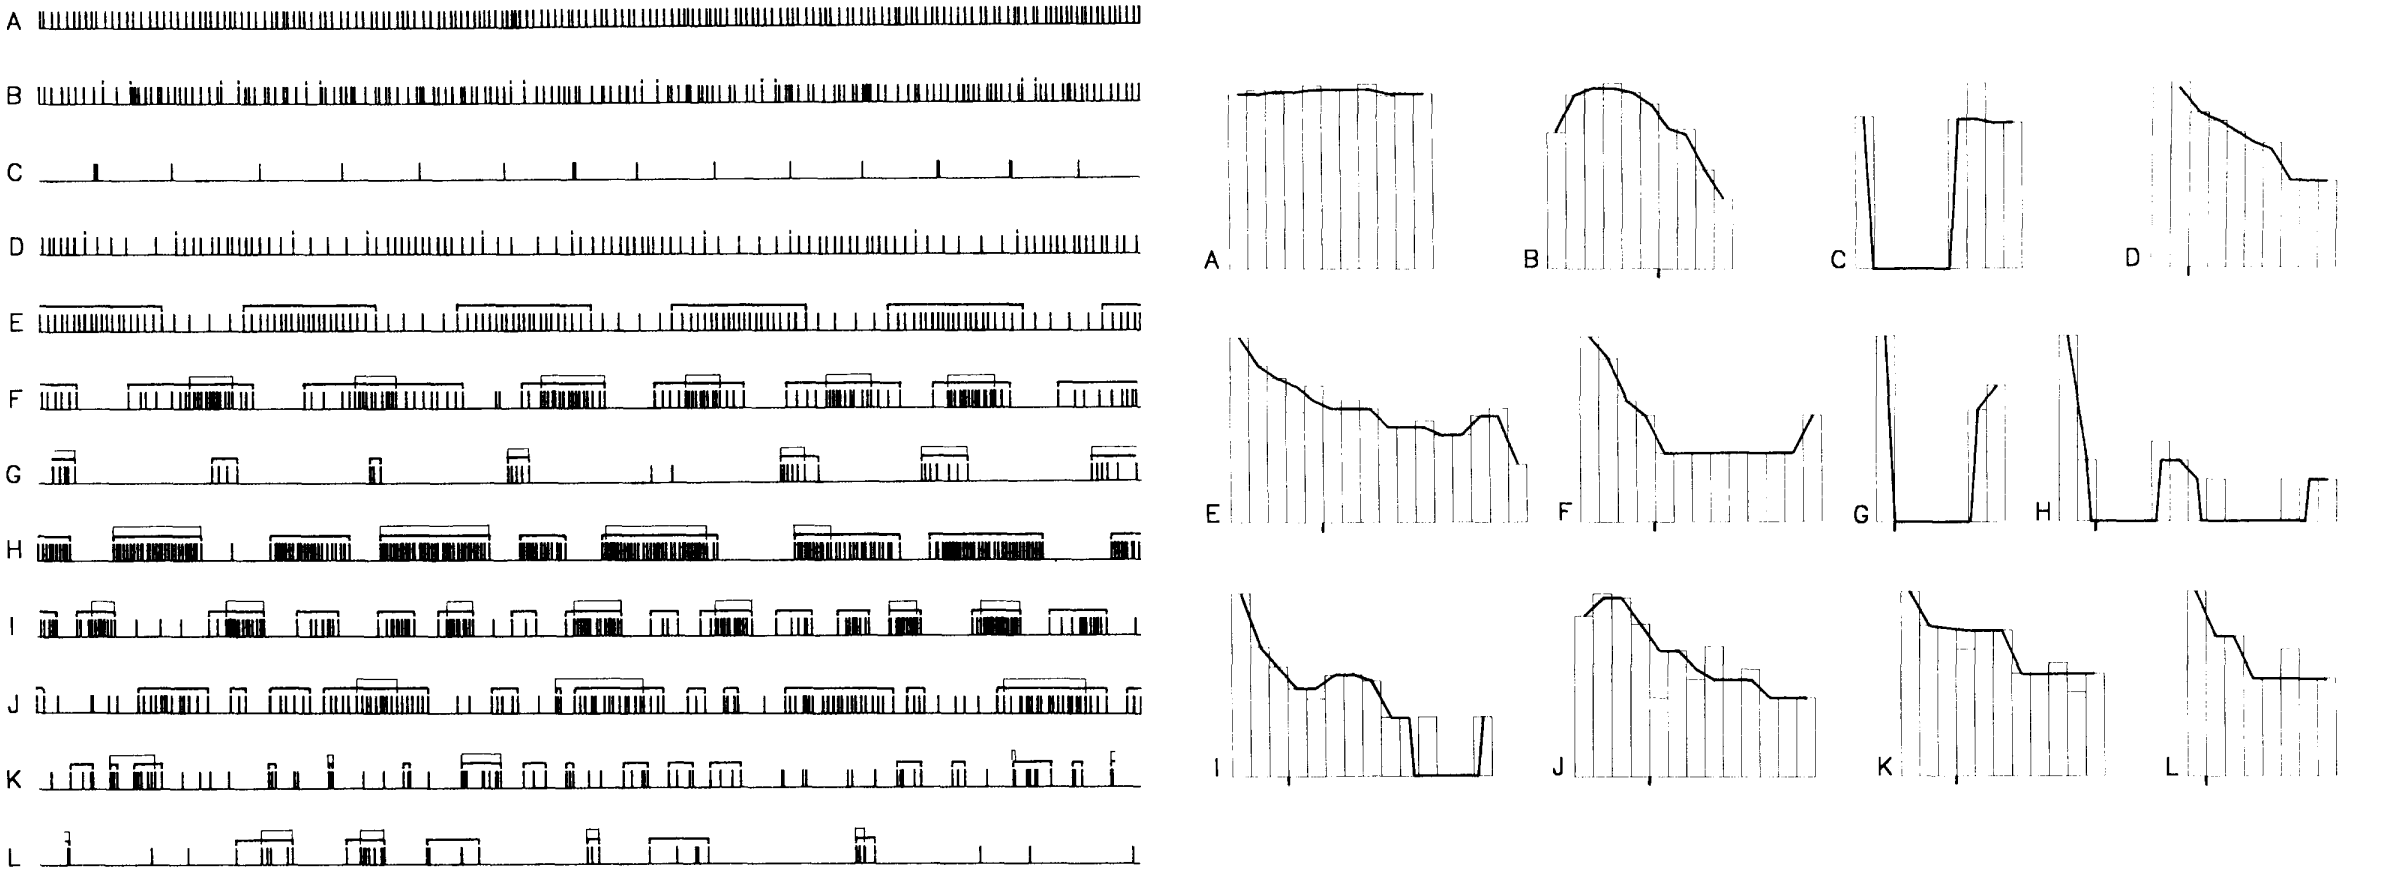
\includegraphics[scale=0.32]{5_3}
    \centering
\end{figure}

\paragraph{Selinger (SE)} This method exploits the ISI histogram (in a logarithmic scale)
to derive the optimal ISI threshold, then it works as a standard single threshold algorithm.
This technique tries to improve the identification of the spikes in the tail portion of a
burst.
\begin{figure}[H]
    \includegraphics[scale=0.5]{5_4}
    \centering
\end{figure}

\paragraph{Modified Selinger (SE-MOD)} Here it is presented a modified version of the
previously explained Selinger method, consisting in a mix of the already presented
techniques. It allows a better identification of the spikes at the boundaries of a
burst event.
\begin{figure}[H]
    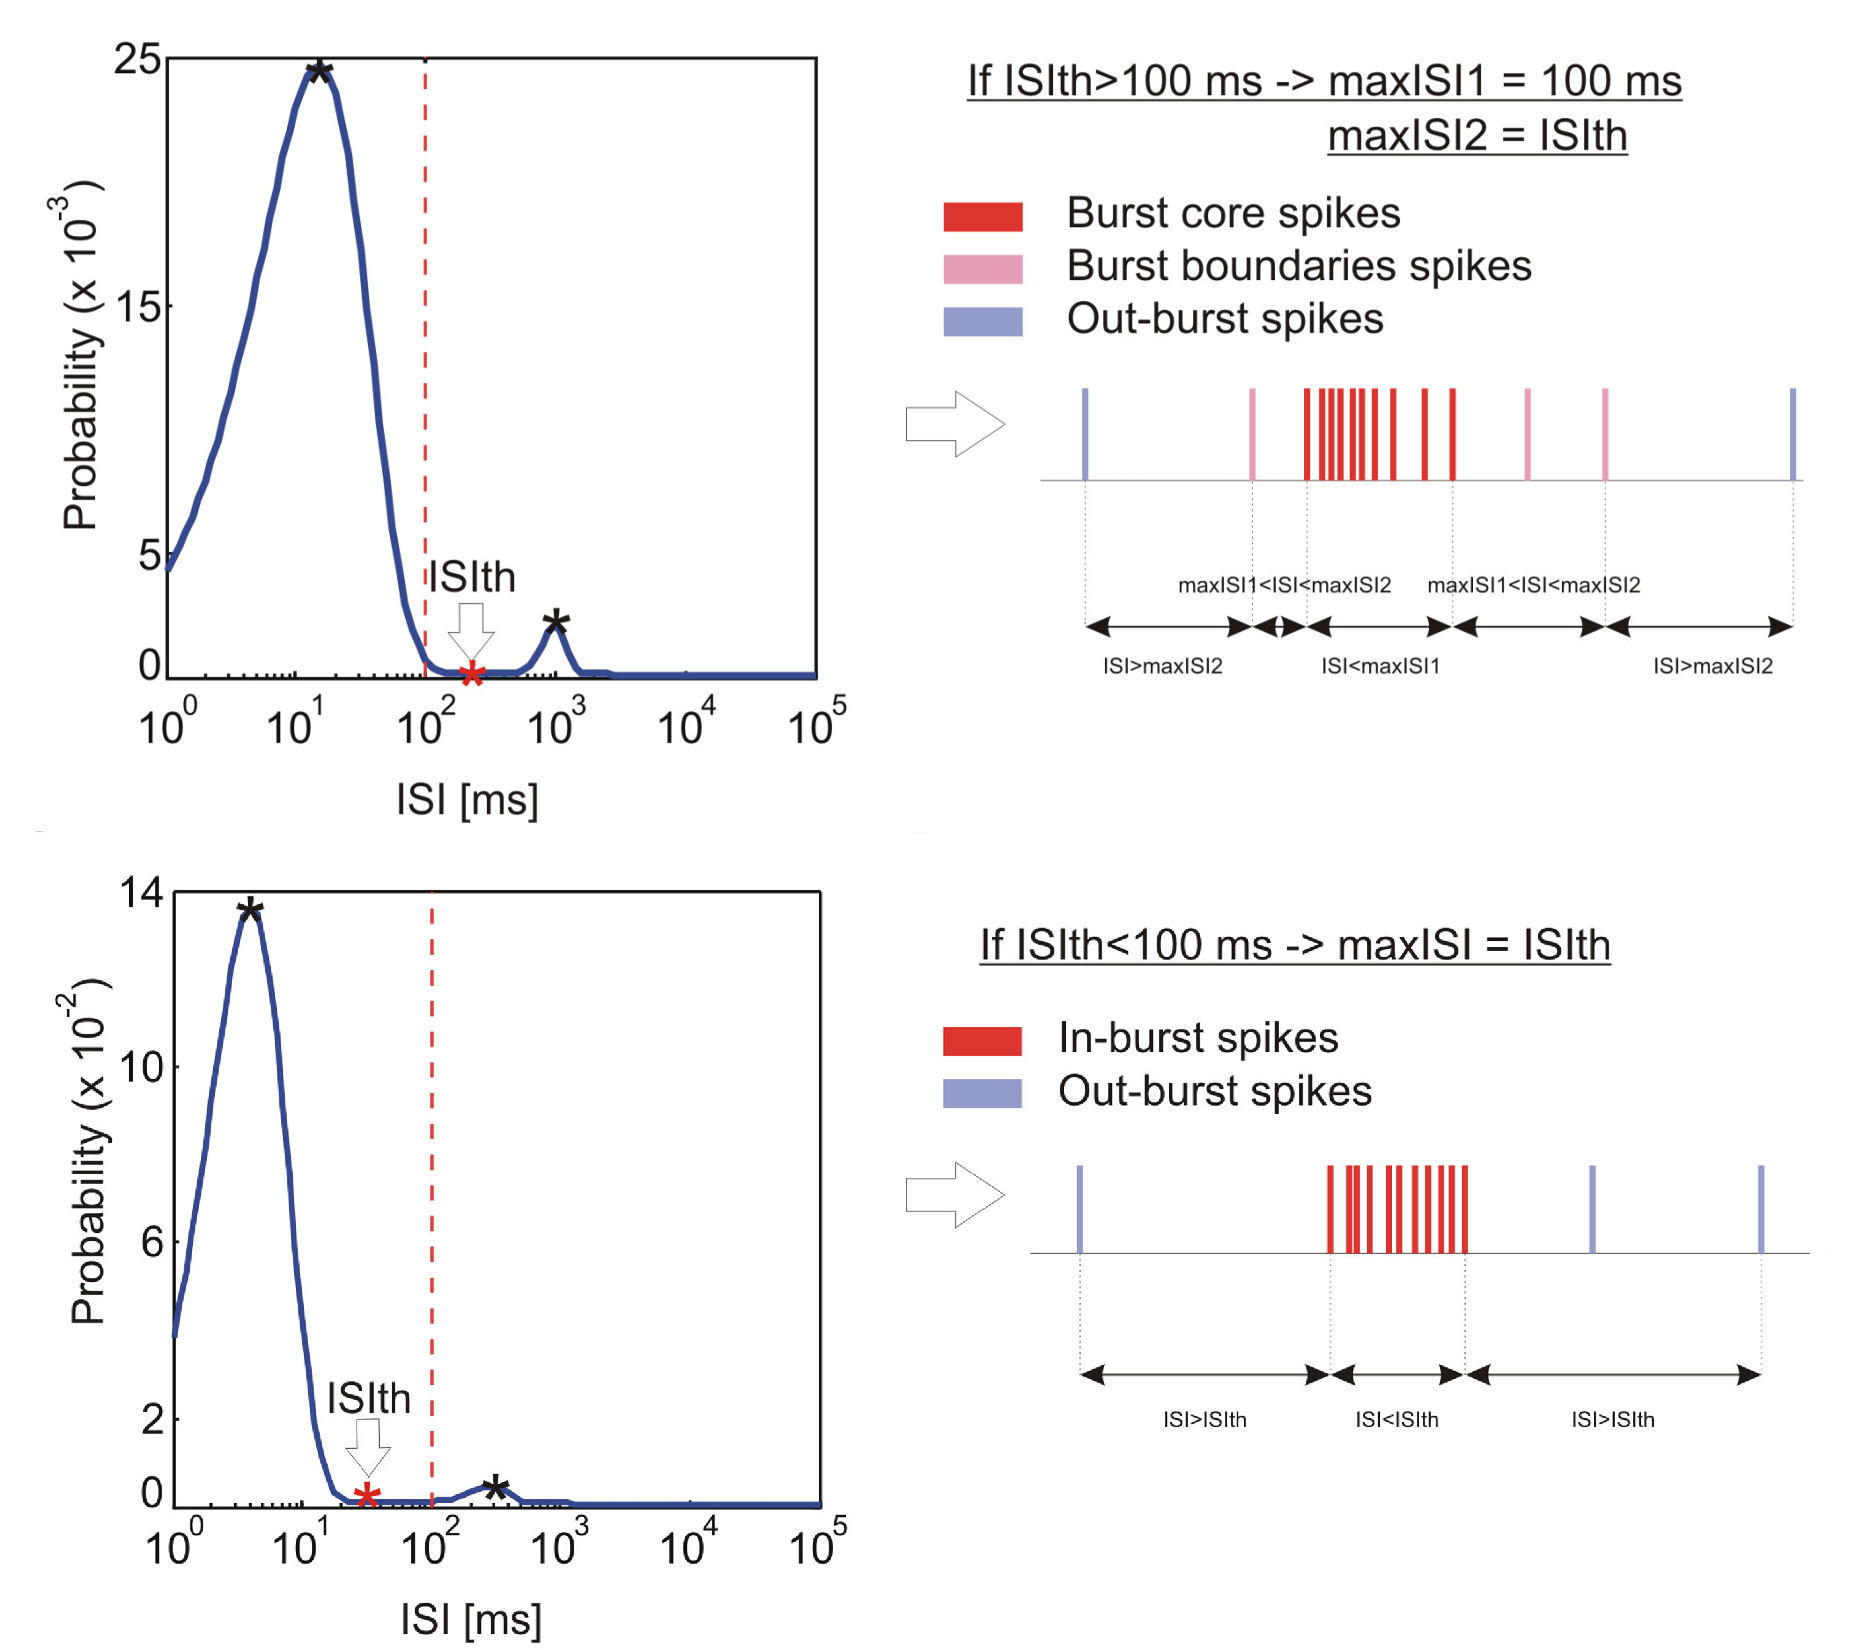
\includegraphics[scale=0.42]{5_5}
    \centering
\end{figure}

Generally, it can be stated that all the implemented burst detection techniques proposed so
far presents pros and cons, thus there is not an algorithm clairly prevailing on the others.
Moreover, different techniques might perform better in different situations, according to
the type of data that are intended to be analyzed.
\newpage

\section{Burst Analysis}
\graphicspath{ {./images/6/} }
\subsection{Introduction}
The burst analysis procedures generate a series of parameters representative for
each burst. The most commonly employed parameters are:
\begin{itemize}
    \item Percentage of bursting channels
    \item Total number of bursts
    \item Mean bursting rate (\(MBR\), expressed in \(bursts/min\))
    \item Burst duration (\(msec\))
    \item Inter burst interval (\(IBI\)): it can be either start-to-start (not
          influenced by burst duration) or end-to-start (influenced by burst duration)
    \item Total number of spikes in a bursting channel
    \item Percentage of random spikes
    \item Mean intra-burst frequency
    \item Peak intra-burst frequency: maximum frequency inside the burst
\end{itemize}
Sometimes it might be useful also to evaluate the out-burst spikes.

\subsection{Data visualization tools}
In the following there is a detailed description of the main tools to characterize and
visualize bursting activity.
\subsubsection{Inter Burst Interval}
The inter burst interval (\(IBI\)) represents the burst equivalent of \(ISI\) for the
spikes. Also in the case of \(IBI\) it is possible to plot an histogram, denominated \(IBIH\).
Bursts are defined as macro-events with a specific duration, which, however, becomes less and
less relevant as the recording period increases, so that in the case of long-term recordings
(tens of minutes), it is possible to consider a burst as a single event.\\
The mathematical formulation of the inter burst interval is given below:
\begin{align*}
    IBIH(\tau)=\frac{1}{M-1}\sum_{b=1}^{M-1}\delta(t_{b+1}-t_{b}-\tau)
\end{align*}
with \(M\) being the total number of burst events.
In a similar way, the analogous concepts of JIBI (Joint IBI, first row of the figure)
and CIBI (Cross IBI, second row of the figure) can be defined.
\begin{figure}[H]
    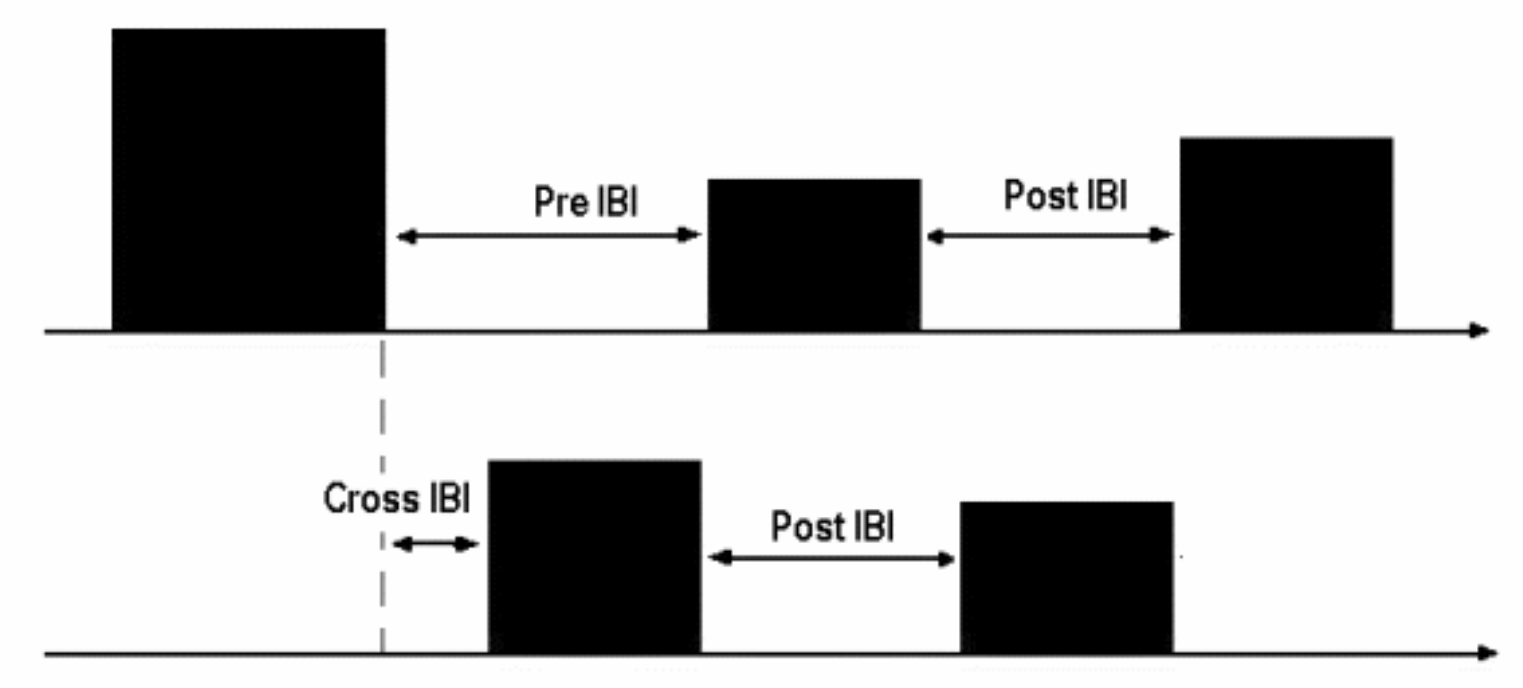
\includegraphics[scale=0.2]{6_1}
    \centering
\end{figure}
\subsubsection{Fano Factor and Coefficient of Variation}
The \textbf{Fano Factor (\(FF\)) dispersion} is a reliable measure of the variability of events
(either spikes or bursts) across a given population. The \(FF\) dispersion is
immediately obtained by computing the average number of events \(\langle{N(T)}\rangle\)
in a time interval \(T\), together with its corresponding variance
\(Var[N(T)]\):
\begin{equation*}
    FF(T)=\frac{Var\bigl[N(T)\bigr]}{\langle{N(T)}\rangle}
\end{equation*}
On the other hand, by replacing the variance with the standard deviation
\(\sigma\bigl[N(T)\bigr]\), one could compute the \textbf{Coefficient of Variation}
\(CV\), that is a little more used:
\begin{align*}
    CV(T)=\frac{\sigma\bigl[N(T)\bigr]}{\langle{N(T)}\rangle}
\end{align*}
Notice that the Coefficient of Variation defined here is exactly the same
measure defined some pages above, denoted as \(C_v\).
\subsubsection{State Space Plot}
This type of representation visualizes data points as function of burst duration
and burst number (or alternatively burst rate). State space plots are
especially valuable to compare the activity of different channels or different
subjects, as they tend to point out differences in the bursts distribution:
for instance, they might be used to show the different activity between two
subjects, one with a pathological condition and the other being totally healthy.
\begin{figure}[H]
    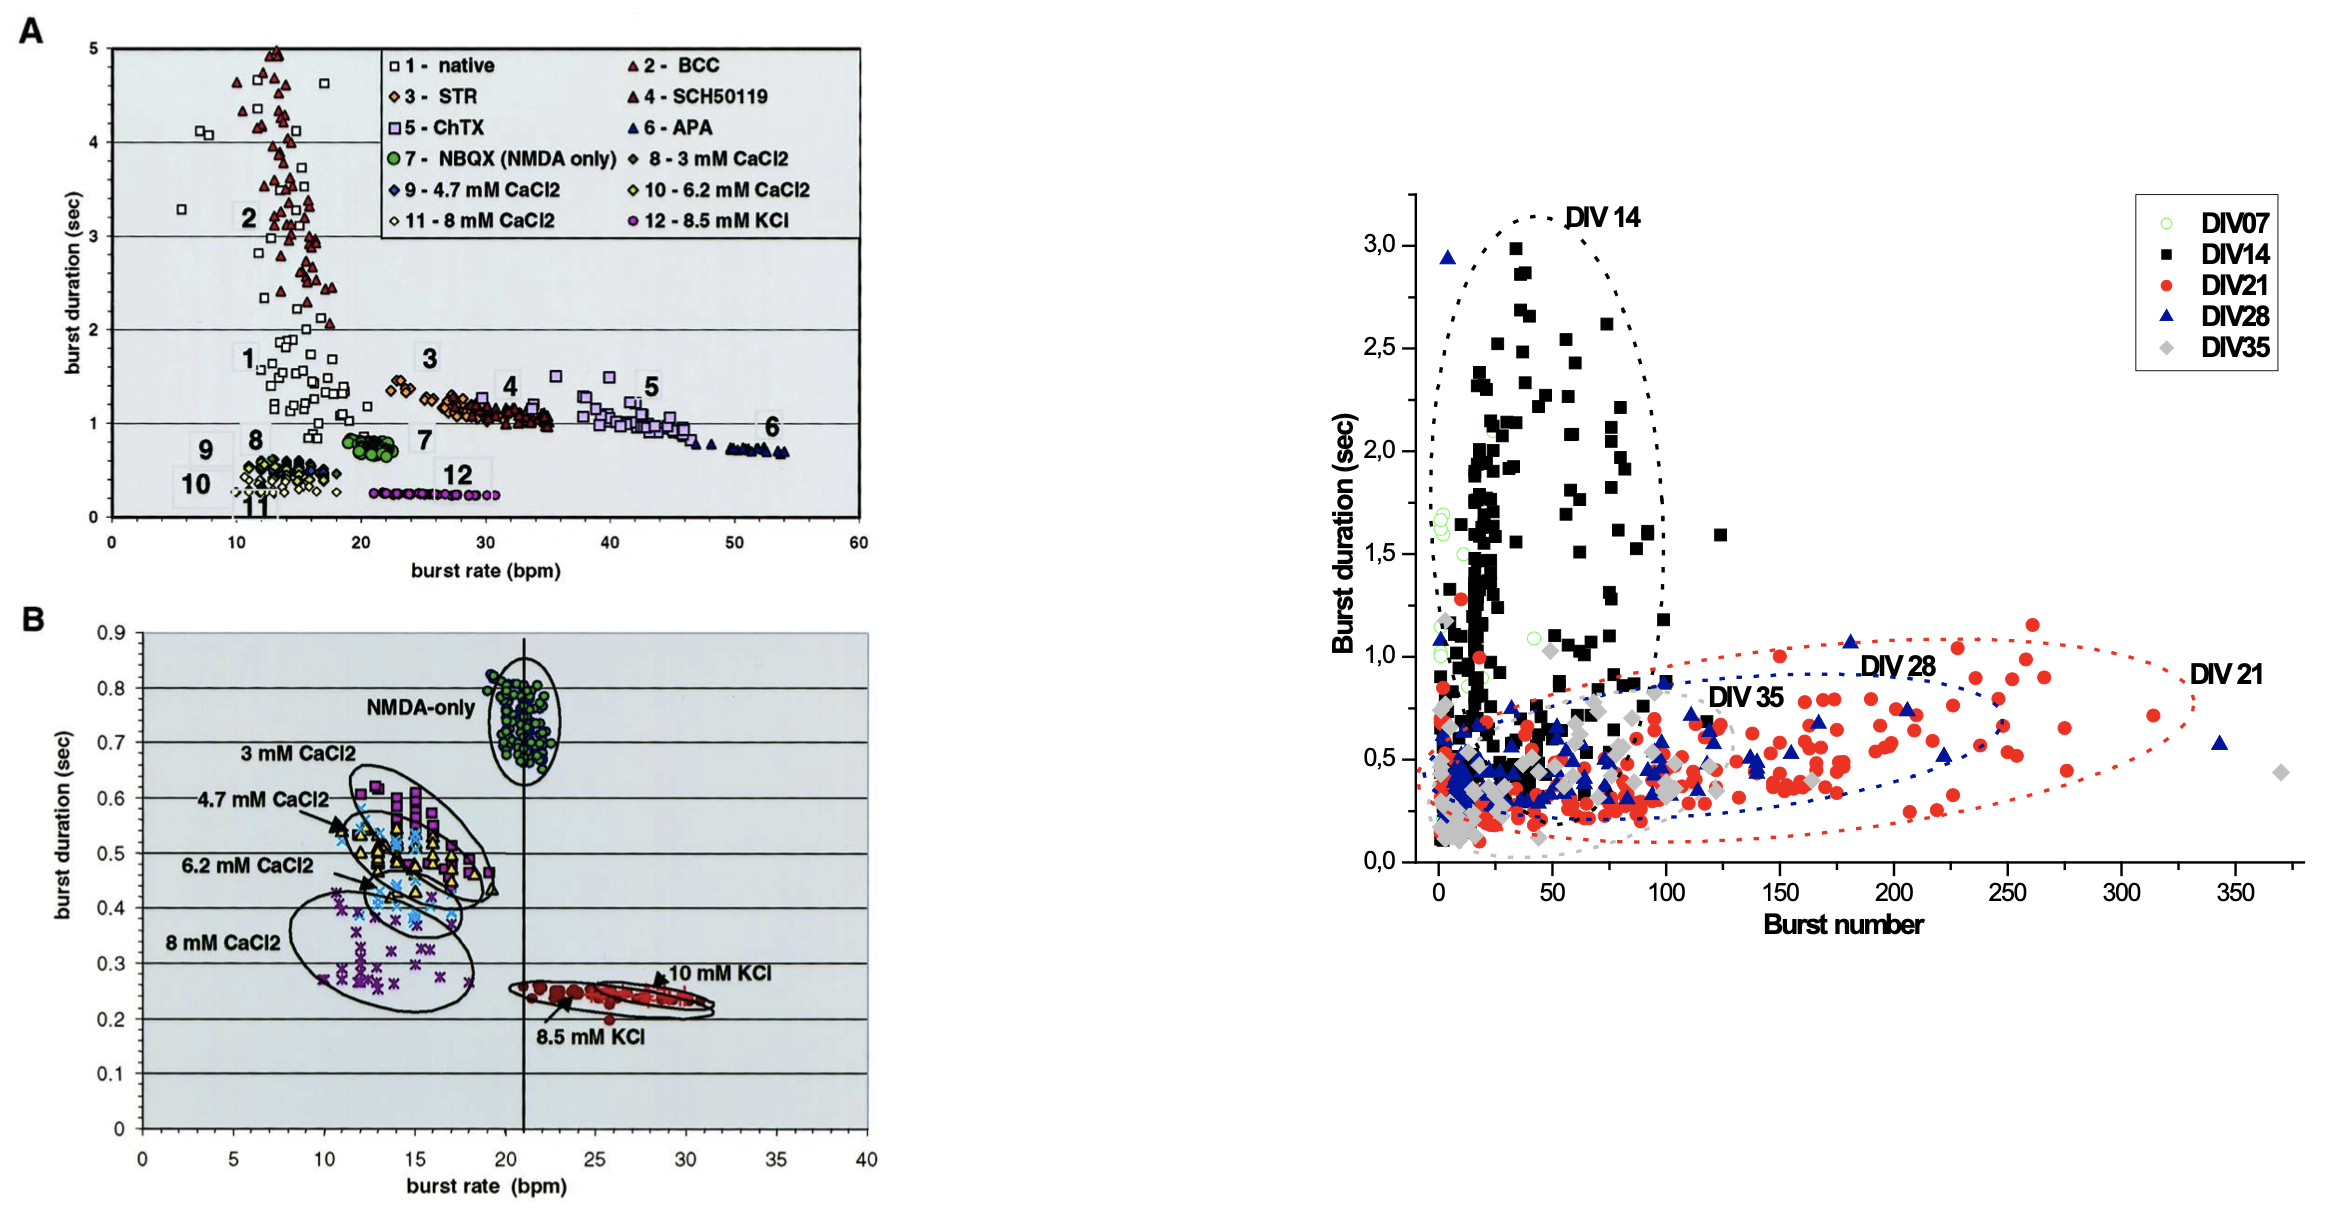
\includegraphics[scale=0.33]{6_2}
    \centering
\end{figure}

\newpage

\section{Network Bursts}
\graphicspath{ {./images/7/} }
\subsection{Introduction}
\textbf{Synchronized activity among neurons} occurs in many brain areas and there are evidences
suggesting that it is relevant for information processing, and, especially, for sensory
processing, cognition and sleep. Patters of reverberating synchronized activity are
believed to reflect neuronal representations of cognitive processes and stored
memories. This kind of synchronized activity is also observed
\textit{in vitro}.\\
A \textbf{network burst (NB)} can be described as a synchronized bursting event involving most units of the network, thus implying that several channels are exhibiting bursting activity at the same time.
\begin{figure}[H]
    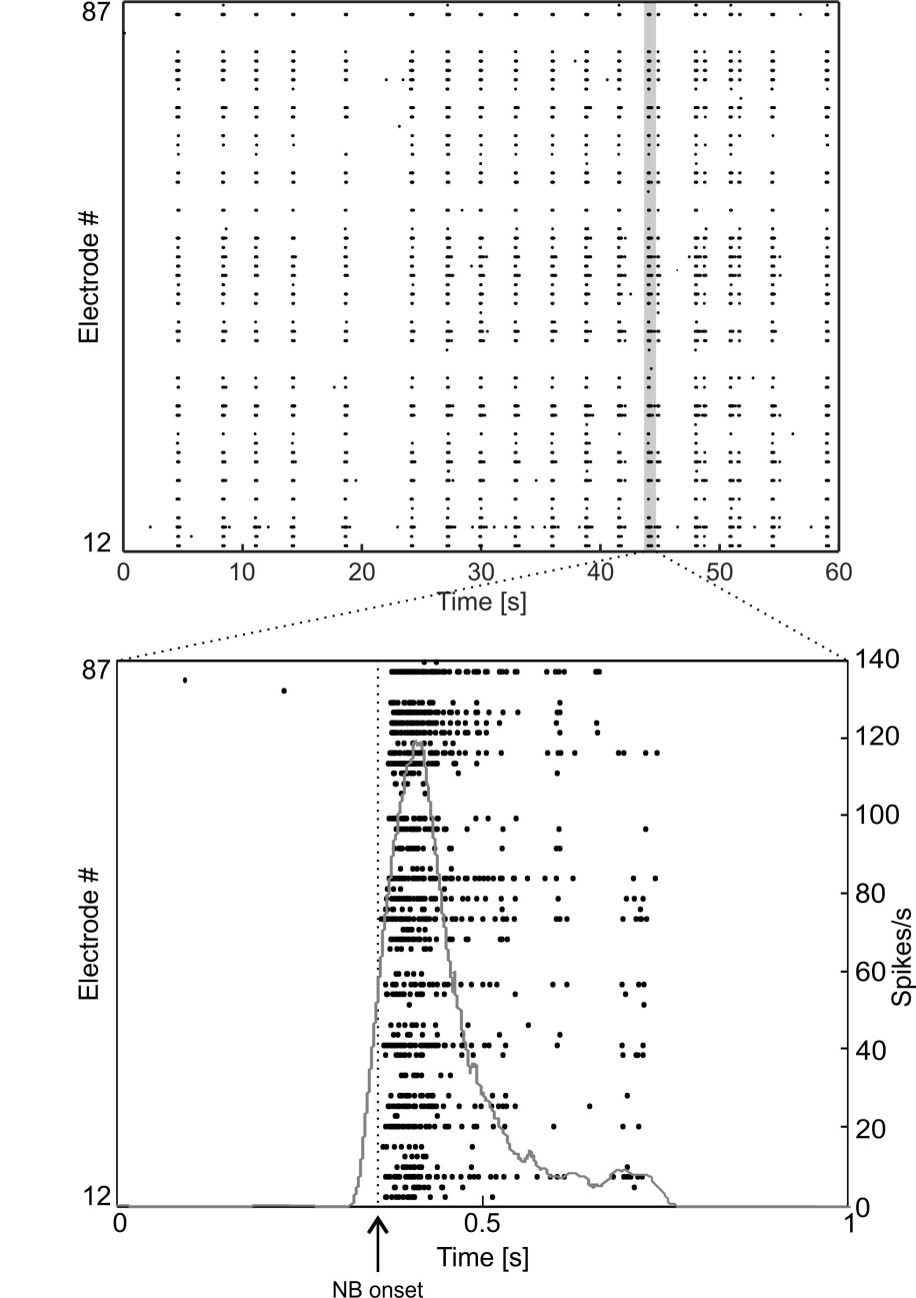
\includegraphics[scale=0.28]{7_1}
    \centering
\end{figure}

\paragraph{LFPs vs MUA}
Network bursting closely reminds to the \textit{UP} and \textit{DOWN} states 
of the \textit{in vivo} cerebral cortex during slow-wave sleep. 
In addition, spontaneous network bursting activity is also easily
noticed in the developing brain, as it is thought to play a key role in
ontogeny (i.e. the origination and development of an organism)
of a neuronal network.\\
In general, it is possible to individuate 6 types of waves, each one described by a typical frequency range:
\begin{itemize}
    \item \textbf{Delta}: \(0.5-4\,Hz\)
    \item \textbf{Theta}: \(4-8\,Hz\)
    \item \textbf{Alpha}: \(8-11\,Hz\)
    \item \textbf{Beta}: \(11-30\,Hz\)
    \item \textbf{Low Gamma}: \(30-55\,Hz\)
    \item \textbf{High Gamma}: \(55-80\,Hz\)
\end{itemize}
\subsection{Example: A Step Into Sleep Physiology}
In mammals and birds, sleeping activity is divided into pretty much different
phases, according to the characteristics exhibited by the brain activity:
\begin{itemize}
    \item \textbf{Rapid Eye Movement (REM):} this phase is also known as \textit{paradoxical
          sleep}. It is characterized by rapid eye movements as well as a rapid low-voltage EEG, similar to the awake state. 
    \item \textbf{Non-Rapid Eye Movement (NREM):} this broad category keeps together
          all the phases where the neuronal activity is considerably different with respect to the awake state. Different NREM stages can be individuated according to the activities:
          \begin{itemize}
              \item \textbf{N1:} it refers to the transition of the brain from alpha waves
                    (awake state with \(f\simeq8-10\,Hz\)) towards theta waves (\(f\simeq4-7\,Hz\)). This stage is often called \textit{drowsy sleep}.
              \item \textbf{N2:} it is characterized by a phenomenon denominated sleep
                    spindles (i.e. bursts of activity), displaying a higher frequency range (\(11-16\,Hz\)). Spindles are related to plasticity and memory. Another typical phenomenon occurring in this stage is K-complexes. 
              \item \textbf{N3:} this stage is commonly denominated \textit{deep sleep} (or \textit{slow-wave sleep}) and it is
                    characterized by the presence of delta waves (at least \(20\%\) of the
                    overall activity) ranging from \(0.5\,Hz\) to \(2\,Hz\). Notice that delta waves exhibit high peak-to-peak voltages (\(>75\,\mu{V}\)).
              \item \textbf{N4:} this stage is usually described as a state in which slow
                    delta waves overcome the \(50\%\) threshold on the total brain oscillatory
                    activity. It is sometimes considered together with stage N3.
          \end{itemize}
\end{itemize}
\begin{figure}[H]
    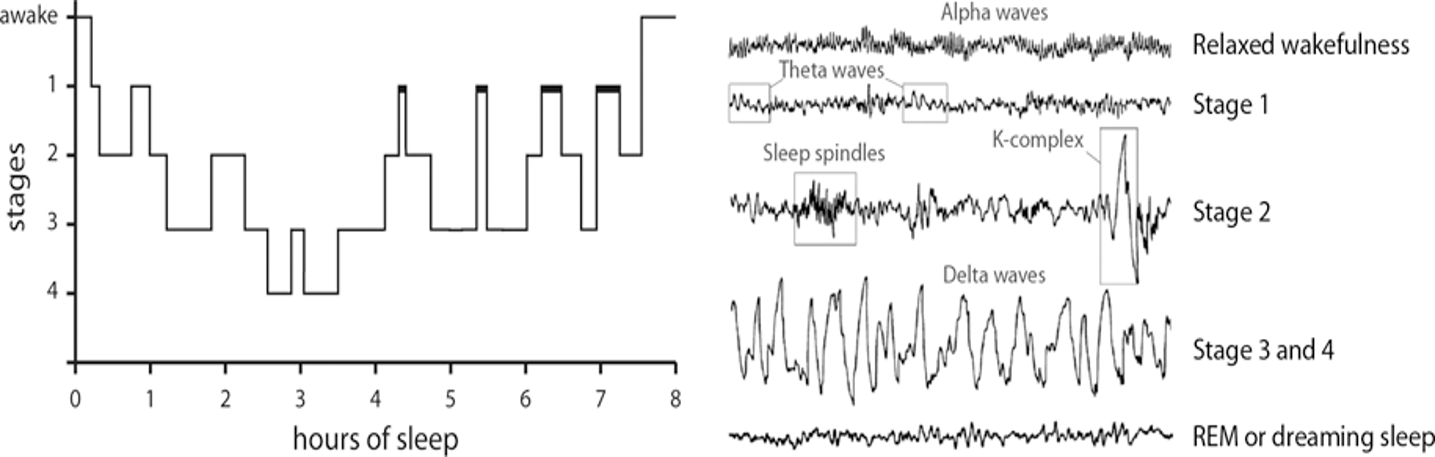
\includegraphics[scale=0.70]{7_2}
    \centering
\end{figure}
There is evidence that network bursting activity is strictly related to the delta waves 
typical of deep sleep, because the periodicity seems to be compatible with the waves during this stage.
\subsection{Network Burst Detection}
In order to detect network bursts, it is necessary to be able to recognize synchronous
increases in the network activity. A number of algorithms have been developed to
solve such a task.
\subsubsection{The Van Pelt algorithm}
Network bursts are short episodes of synchronized firing among many recording sites. They are not
exclusively described by increased firing rates at individual sites, but also by an
increase of the number of active sites.\\ 
The Van Pelt algorithm consists in dividing the time
axis into a number of small bins and computing the product between the number of
active sites (i.e. the recording channels showing firing activity) and the total
number of spikes at these sites. In case of uncorrelated spiking activity among
the sites, this product won't significantly differ from the total spike count, however
it raises sharply as soon as the firing becomes synchronized. The time point at
which the product reaches its maximum value is used to
define a center-of-mass-based time center of the network burst.
\begin{figure}[H]
    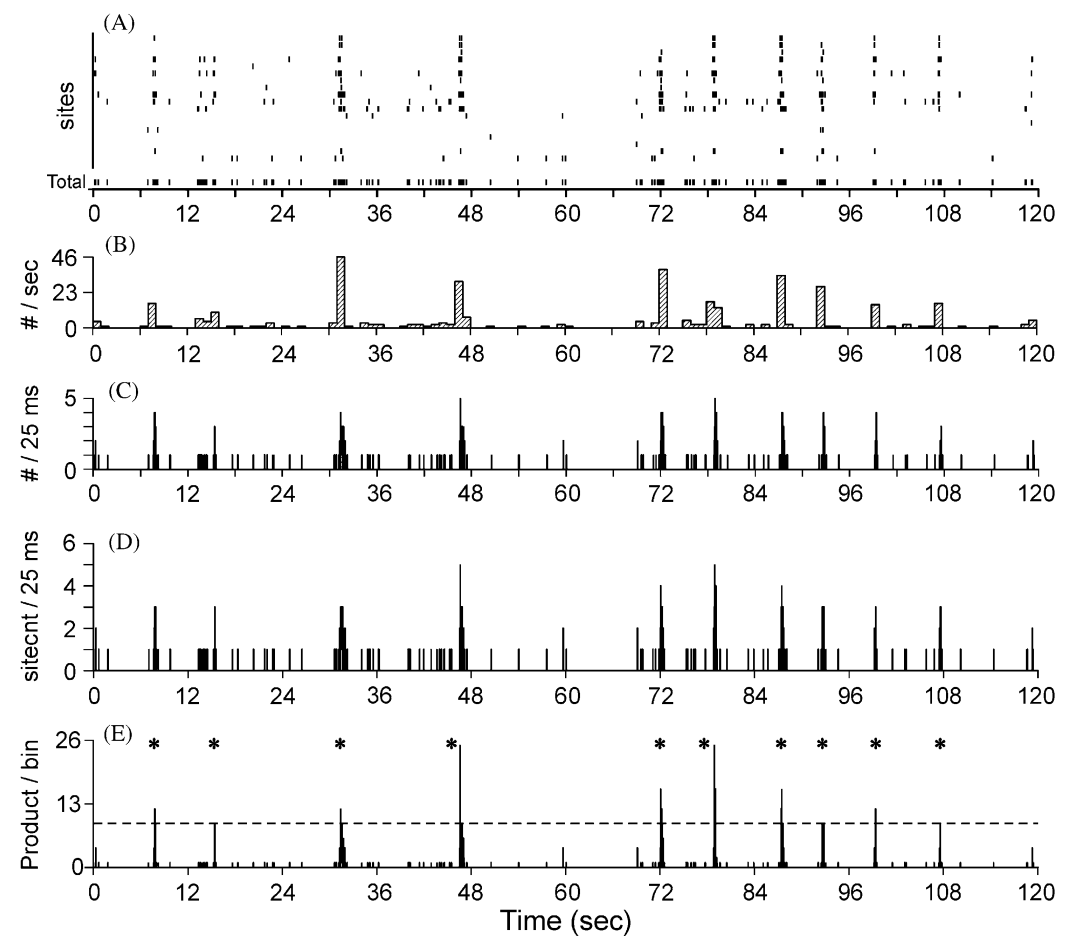
\includegraphics[scale=0.6]{7_3}
    \centering
\end{figure}
\pagebreak
The last figure shows the network burst detection procedure:
\begin{itemize}
    \item[(A)] The time points of spikes at the different recording sites of
          a multi-electrode array. The lowest trace shows the total spike train for all
          the sites.
    \item[(B)] A total network firing rate plot with time bins of \(1\,s\).
    \item[(C)] A total network firing rate plot with time bins of \(25\,ms\).
    \item[(D)] A plot of the number of active sites with time bins
          of \(25\,ms\).
    \item[(E)] A plot of the product of total number of spikes and the
          number of active sites, calculated per \(25\,ms\) time bins. The dashed line
          represents a threshold to overcome to identify an actual network burst, which
          are individuated by a star.
\end{itemize}
Having the raster plot, a division with bins of \(25\,ms\) can be performed. This can tell if there are times in the recording with an increased activity. Then, an improvement is to consider not only the spike count, but also how many channels are active in the same bin. It should be better to avoid to have 1 channel with 1 burst and 20 with 0 bursts, but if there is a channel with many bursts, then it should be considered in a different way.
\subsubsection{The LogISI method}
This technique requires that burst detection has been performed for every
recording channel. Then, a burst event train for each channel is derived, where
bursts are described as single point events, disregarding every information about
their duration. These points for all the sites are then projected onto the same axis.
At this point, burst detection is performed again on this new axis, allowing
to look for time periods with an increased bursting activity on several channels (thus
synchronized). Therefore, this algorithm consists in an iterative application of burst detection procedures.\\
Notice that the minimum number of intra-burst spikes for the cumulative
burst event train can be intended as the minimum number of active channels required
to detect a network burst event, usually set as the \(20\%\) of the total number of
recording sites.
\begin{figure}[H]
    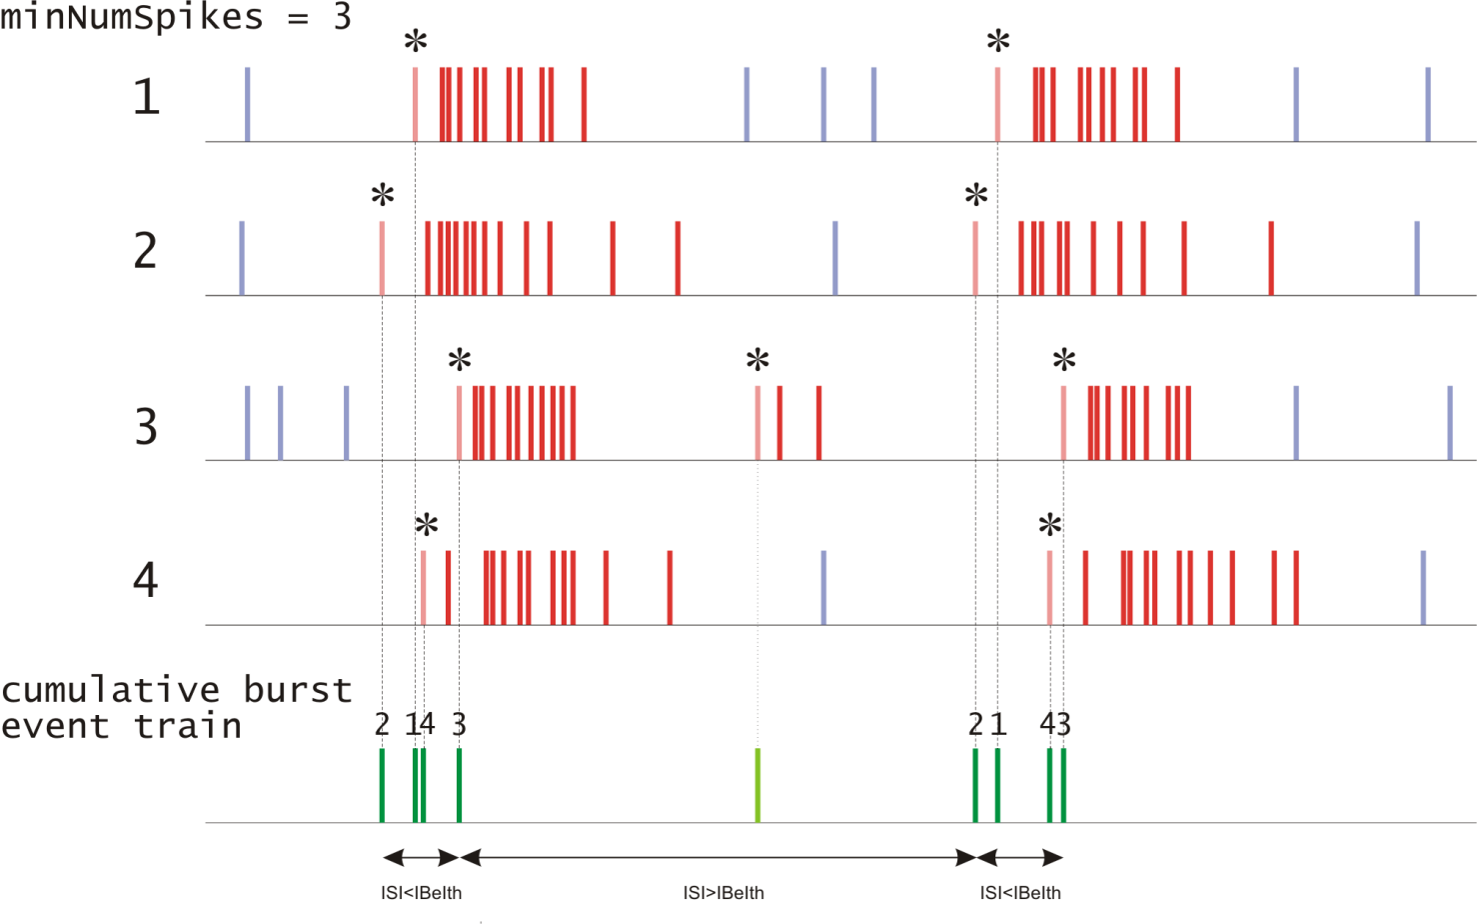
\includegraphics[scale=0.65]{7_4}
    \centering
\end{figure}

\subsection{Metrics}
Some of the most relevant metrics to characterize network bursting are reported
in the following.
\subsubsection{The Burstiness Index}
The burstiness index (\(BI\)) is a metric, empirically derived by D. A. Wagenaar in order to assess the burstiness
of a neuronal network with just one number. From experiments, it has been noticed that,
in general, the overall time occupied by network bursts in a whole recording is
always less than \(15\%\) of the total duration, and this factor has been taken as an
assumption for the computation of constants employed to derive the burstiness
index.\\ 
The computation steps are reported here:
\begin{enumerate}
    \item Divide a 5 minutes recording into time bins (each 1 second long), obtaining 300 of them.
    \item Count the total number of spikes for each bin, across all the recording sites.
    \item Compute the fraction of the total number of spikes contained in the \(15\%\)
          of bins with the largest counts, indicated as \(f_{15}\).
          \begin{itemize}
              \item If the firing rate is tonic, then \(f_{15}\) is expected to be close to \(0.15\).
              \item If a recording is bursty, it is more likely that most of the spikes will
                    be contained in bursts, resulting in \(f_{15}\) close to \(1\).
          \end{itemize}
    \item Compute the \textbf{burstiness index} normalized between \(0\) and \(1\) as
          \begin{align*}
              BI = \frac{f_{15}-0.15}{0.85}
          \end{align*}
\end{enumerate}
\subsection{Major Burst Leaders}
Each network burst spreads through the recording sites according to a specific
spatio-temporal pattern, resulting in a precise sequence of electrodes activation.
Major Burst Leaders (MBLs) are the privileged nodes in the network that consistently
fire earlier than the others at the onset of the network bursts. It is critical to
individuate them, as they play the role of leaders of the synchronized bursting
activity. The pool of MBLs is stable across hours, although the leadership frequency of individual channels may vary.\\
In general, MBLs are not unique. The first firing neuron in the network burst is called \textbf{Burst Leader} (BL) and, looking at the definition, 
it is intuitive the fact that the BL is unique, even if it may change in time, being one of the MBLs but not always the same.
\newpage
Each node is given a certain leadership score, as shown in the following figure, according
to its relevance in the initiation of a bursting event. If such score overcomes a
certain threshold (indicated by the dotted line), then the node is identified as
one of the MBLs.
\begin{figure}[H]
    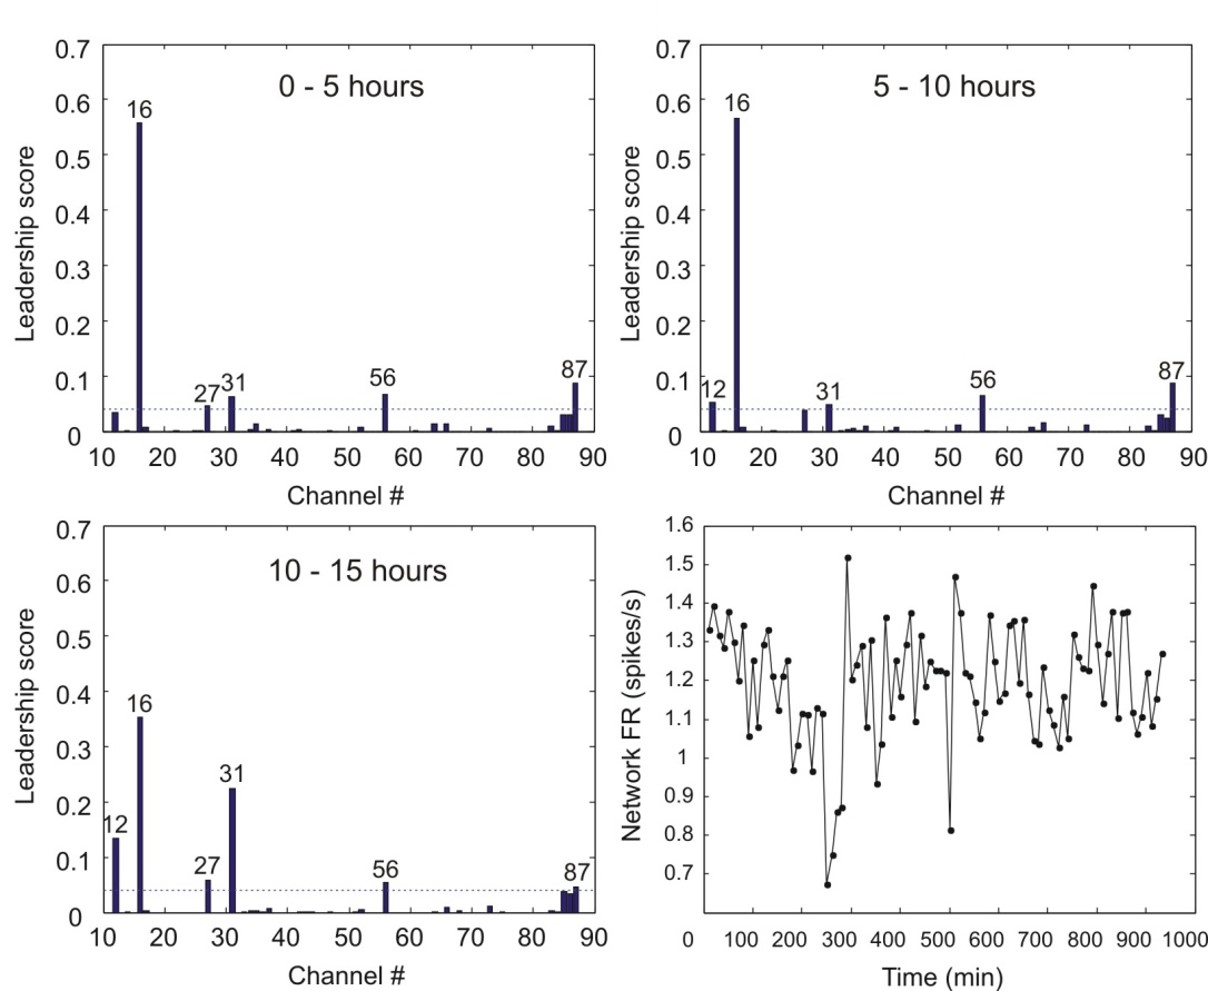
\includegraphics[scale=0.7]{7_5}
    \centering
\end{figure}
Another crucial phenomenon is the recruitment of MBLs. In fact,
as soon as MBLs are activated, they recruit other MBLs in the network burst pathway, where by recruitment it is meant
the activation of other nodes in order to facilitate the initiation of a network burst.
In addition, MBLs are involved in network bursting activity with a higher reliability
than other common nodes (\(>90\%\)).
\begin{figure}[H]
    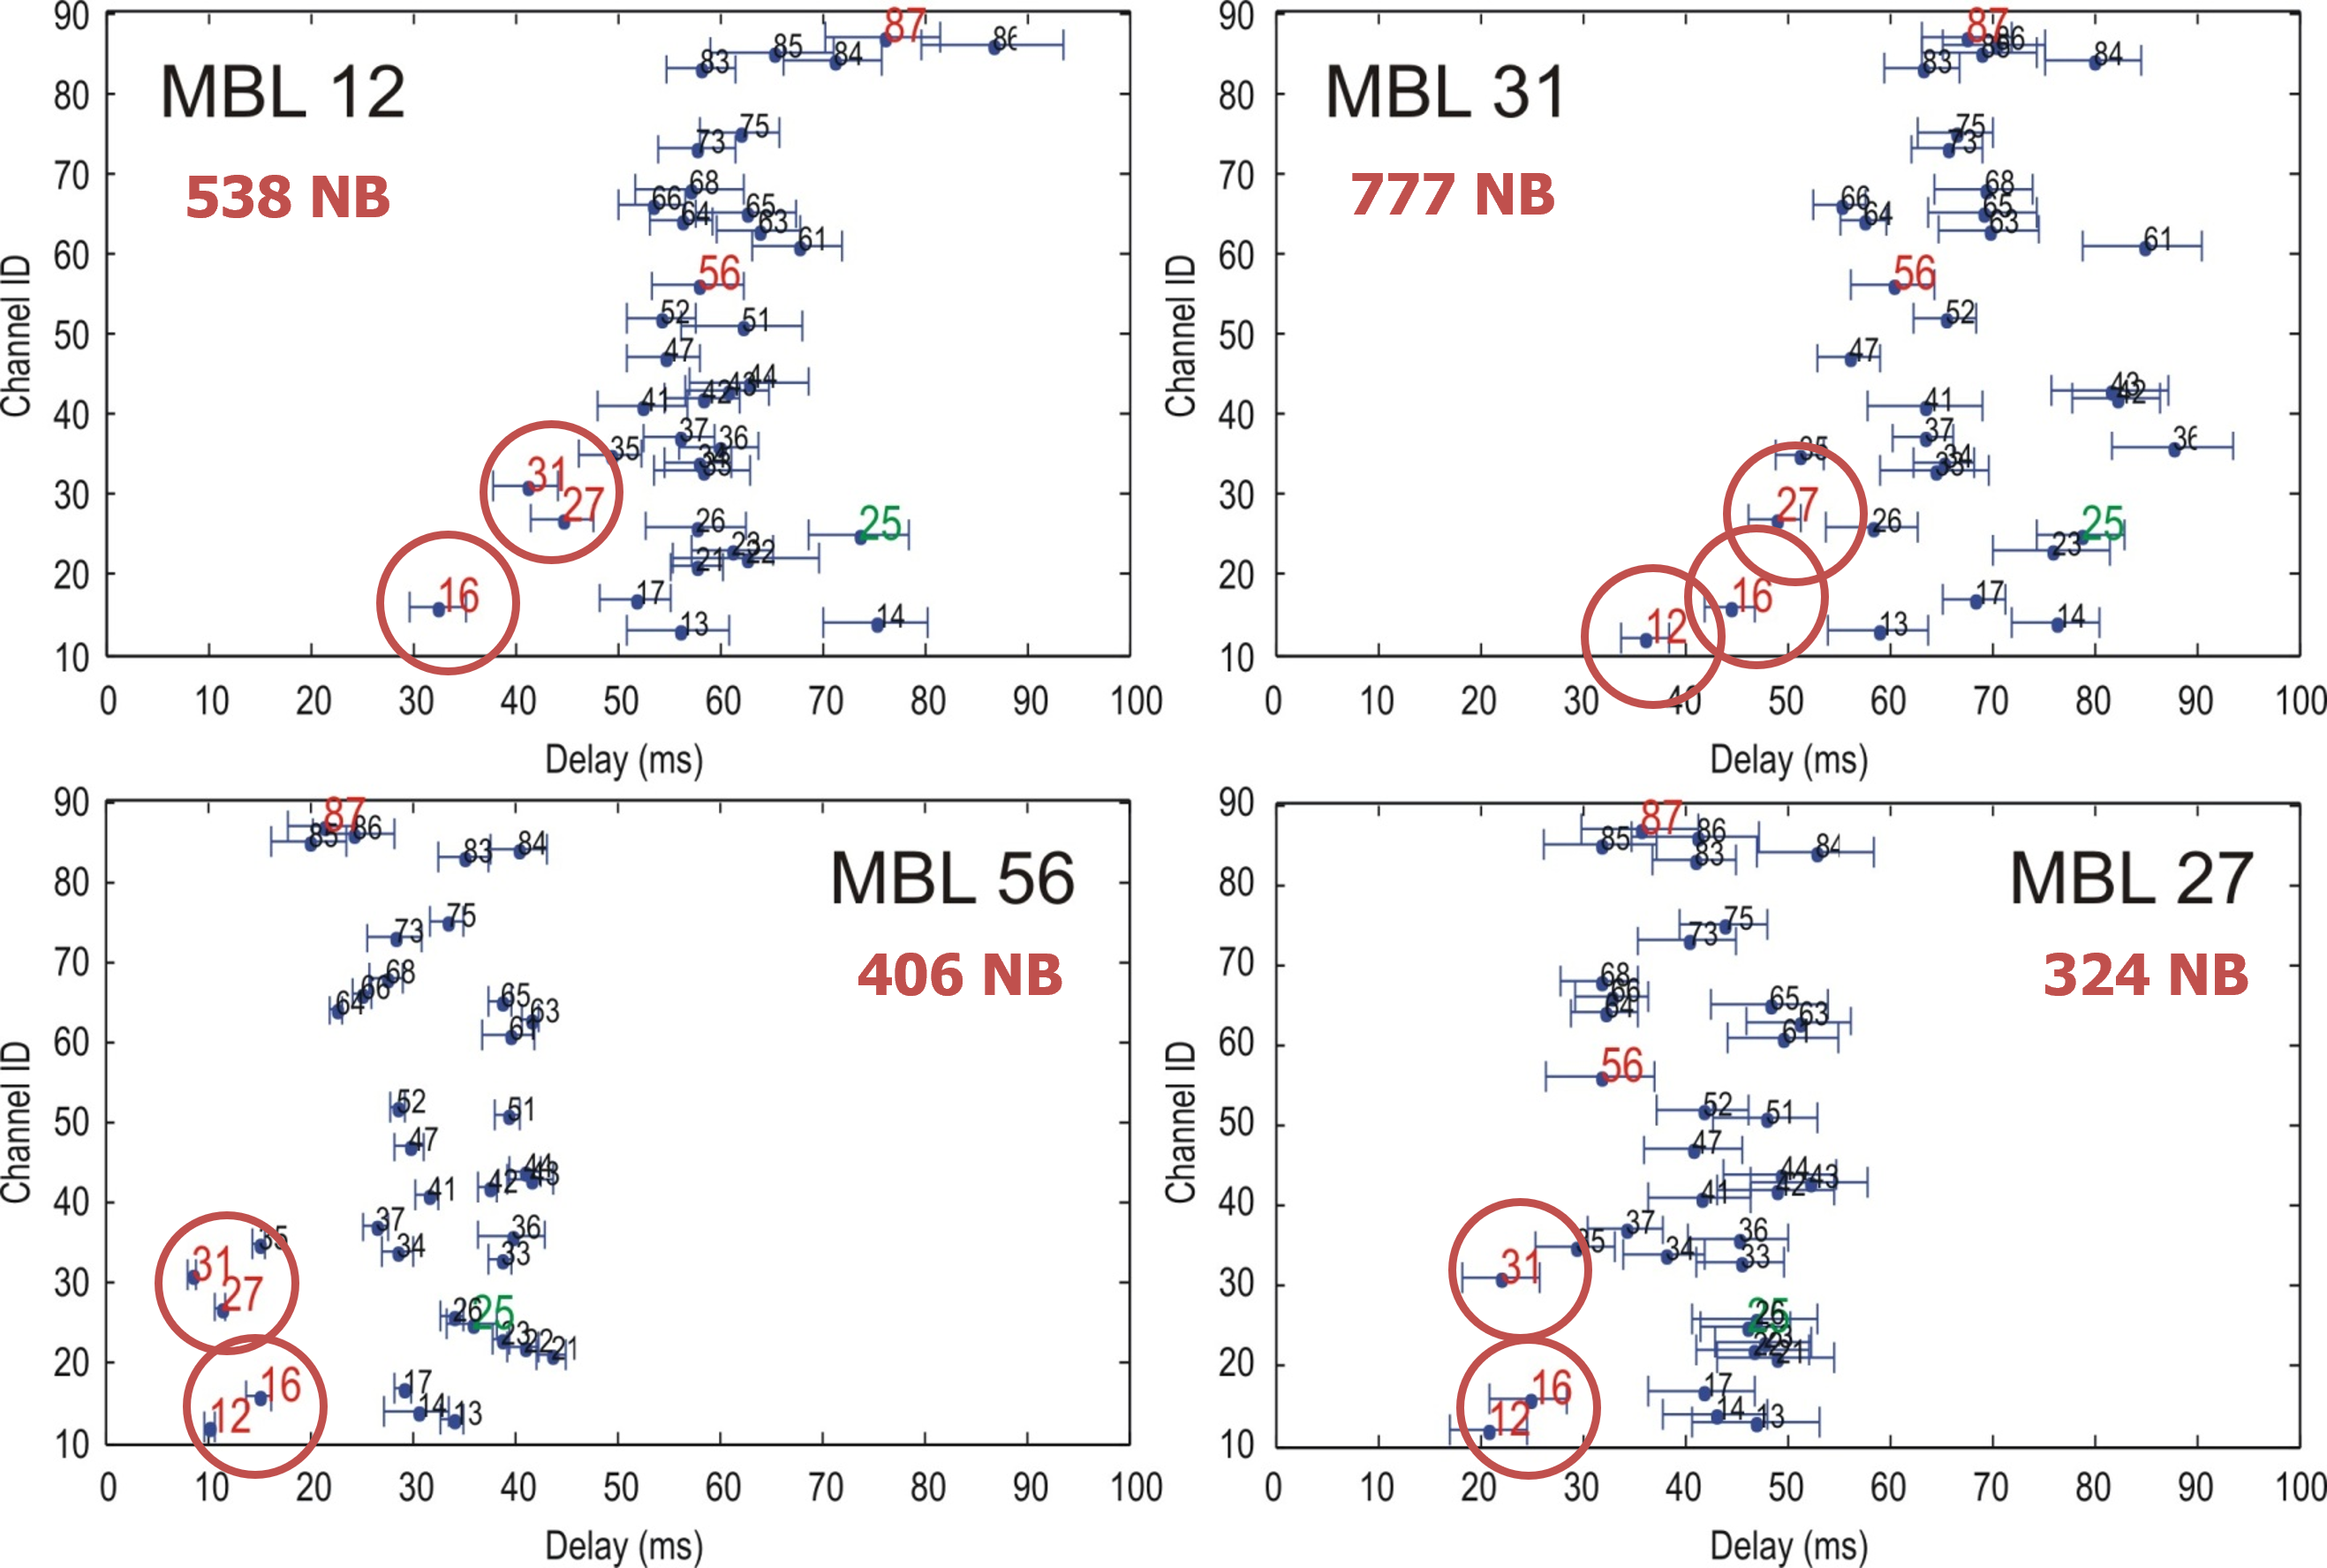
\includegraphics[scale=0.65]{7_6}
    \centering
\end{figure}
At this point, one might wonder if MBLs represent the most active channels in terms
of spikes. Although no correlation between the leadership score and the fraction of
spikes outside network bursts has been assessed, it has been observed that almost
all MBLs have a sustained spiking activity, with an average firing rate higher than
the network average. Moreover, it seems that their response to electrical stimulation
is indeed stronger and faster than the one of common neurons.
\begin{figure}[H]
    \includegraphics[scale=0.7]{7_7}
    \centering
\end{figure}
A possible interpretation of this phenomenon could be that MBLs receive a large number
of incoming excitatory connections, acting as \textbf{network hubs}, integrating
several inputs and redistributing them to the network.
\newpage

\section{Further Analysis Tools}
\graphicspath{ {./images/8/} }
\subsection{Introduction}
Spike trains can be analyzed by exploiting several kinds of techniques, according
to the aim of the analysis. In particular, it might be interesting to study the
behaviour of a recording site after an external stimulation. Notice that this kind
of analysis becomes more and more relevant as it is extended to multiple channels, for
instance in order to study how different neurons react to the same stimulus.
Alternatively, the responses from several subjects can be compared as well. Other
interesting analyses might consist in comparing several channels or corresponding
channels in different subjects, establishing proper metrics to assess similarity
and correlation.

\subsection{Post Stimulus Time Histogram}
Post Stimulus Time Histogram (PSTH) is a vital tool to characterize neural spike trains
in response to a stimulus. Notice that in general the response of a certain neuron
for a repeated given stimulus is not identical, but it tends to change, as in the
adaptation phenomenon.\\
The intensity of the response and its dynamics is visualized through an histogram.
As a matter of fact, a certain time window is isolated after the occurrence of the
stimulus and it is divided into several equally long bins. Then, the total number of
spikes in each bin is counted and reported into the histogram, as shown in the figure
below.
\begin{figure}[H]
    \includegraphics[scale=0.75]{8_1}
    \centering
\end{figure}
Notice that the spike count can be normalized in order to obtain the firing rate, which
can be interpreted also as the probability of firing per time unit.\\
As already state, it is possible to derive several distinct kinds of PSTH, according to
the use case. It can be computed for a single neuron or a single recording site. It
can be computed distinctly for each site of a multi-channel recording, generating
a large number of PST histograms. On the other hand, an averaged PSTH is commonly used
to asses the average response of a network with several recording sites. Nonetheless,
an average PSTH is also employed to consider together spike trains generated in
multiple trials or subjects.
\begin{figure}[H]
    \includegraphics[scale=0.3]{8_2}
    \centering
\end{figure}
Generally, after after being stimulated, a neuron exhibits two different responses:
\begin{itemize}
    \item \textbf{Early response:} it occurs in the first \(50\,ms\) after the stimulus
          and includes the direct activation of the neuron.
    \item \textbf{Late (or delayed) response:} it occurs at least after \(50\,ms\) and up to
          \(400\,ms\), representing a reverberating response.
\end{itemize}
It can be said that the early response is definitely more reliable than the late
response, as the second one might be influenced by noise. A way to better focus
on the early response direct activation consists in chemically blocking the synapses.
\begin{figure}[H]
    \includegraphics[scale=1.75]{8_3}
    \centering
\end{figure}
In addition, PST histograms might represent a valuable tool to individuate Major Burst
Leaders (MBLs), as they highlight the rapidity of a neuron to produce a response. In the
following picture a PSTH for each channel of an array of electrodes is represented,
according to the physical layout of the electrodes, and the MBLs are highlighted in red.
\begin{figure}[H]
    \includegraphics[scale=0.6]{8_4}
    \centering
\end{figure}

\subsection{Cross-Correlation}
The cross-correlation between spike trains is a fundamental metric, as it is capable
to highlight synchronization phenomena at the network level. Notice that this metric
can alternatively be computed starting from the spike trains or the burst trains.
A train is defined as the reference train, identified by \(x\), while the other
one is employed as the target train, denoted by \(y\).\\
The two trains are divided into equally spaced bins small enough to contain at most
one spike, then a cross-correlogram - i.e. a cross-correlation histogram - is derived
by counting the number of bins displaying a spike in both the reference and the target
trains. A time delay \(\tau\) is applied as a variable shift between the two trains.
Notice that by switching the reverse and the target trains, the same plot is obtained,
but reversed in the horizontal time axis.
\begin{figure}[H]
    \includegraphics[scale=0.9]{8_5}
    \centering
\end{figure}
From a mathematical point of view, the cross-correlation \(C_{xy}\) can be formalized
as follow:
\begin{align*}
    C_{xy}(\tau)
    =\sum_{s=1}^{N_x}\sum_{t_{i}=(\tau-\Delta{\tau}/2)}^{(\tau+\Delta{\tau}/2)}x(t_s)y(t_s-t_i)
\end{align*}
Notice that a normalization term can be easily added in order to provide
a cross-correlation value in the \([0, 1]\) range:
\begin{align*}
    C_{xy}(\tau)
    =\frac{1}{\sqrt{N_xN_y}}\sum_{s=1}^{N_x}\sum_{t_{i}=(\tau-\Delta{\tau}/2)}^{(\tau+\Delta{\tau}/2)}x(t_s)y(t_s-t_i)
\end{align*}
where \(N_x\) is the total number of spikes in the reference train and \(N_y\) is the
total number of spikes in the target train. The previously described properties of
\(C_{xy}(\tau)\) can be summarized as follow:
\begin{itemize}
    \item \(0\le{C_{xy}(\tau)}\le{1}\)
    \item \(C_{xy}(\tau)=-C_{yx}(\tau)\)
\end{itemize}
Auto-correlation is often used to test the functioning of a cross-correlation
algorithm:
\begin{align*}
    C_{xx}(\tau)
    &=\frac{1}{\sqrt{N_xN_x}}\sum_{s=1}^{N_x}\sum_{t_{i}=(\tau-\Delta{\tau}/2)}^{(\tau+\Delta{\tau}/2)}x(t_s)x(t_s-t_i) \\
    &=\frac{1}{N_x}\sum_{s=1}^{N_x}\sum_{t_{i}=(\tau-\Delta{\tau}/2)}^{(\tau+\Delta{\tau}/2)}x(t_s)x(t_s-t_i)
\end{align*}
\begin{figure}[H]
    \includegraphics[scale=0.9]{8_6}
    \centering
\end{figure}
A further mean-correlogram can be computed to assess how one channel is correlated
to all of the others:
\begin{align*}
    C_x(\tau)=\frac{1}{n-1}\sum_{y=1}^{n}C_{xy}(\tau)
\end{align*}
It is now possible to define the cross-correlation function in zero \(C(0)\), with
the bin centered in zero:
\begin{align*}
    C(0)=\sum_{\tau=-k(\Delta\tau/2)}^{k(\Delta\tau/2)}C_{xy}(\tau)
\end{align*}
with \(\Delta\tau\) being the bin size and \(k\) indicating the considered number of
bin around the central one, identified as bin zero.
On the other hand, the \(C_{peak}\) represents the value of the cross-correlogram in
an area around the maximum detected peak. This is computed in order to quantify the
correlation level among all the recording channels. The peak latency is the distance
of the maximum peak from the zero: it can be interpreted as the delay of an
estimated functional connection.
\begin{align*}
    C_{peak}=\sum_{\tau=\tau_{peak}-k(\Delta\tau/2)}^{\tau_{peak}+k(\Delta\tau/2)}C_{xy}(\tau)
\end{align*}
Two channels can be considered to be synchronized whenever the central peak is
centered in zero, implying a very small peak latency.
\begin{figure}[H]
    \includegraphics[scale=0.9]{8_7}
    \centering
\end{figure}
\newpage

\section{Meso-scale: Recording and Origin}
\graphicspath{ {./images/9/} }
\subsection{Introduction}
Generally, it can be affirmed that different parts of the brain are responsible
for different actions as well as respond to different sensory inputs. It is
thought to be the most complex organ of the body, moreover it consumes more or less
\(20\%\) of the overall ATP produced. The cortex is made of approximately \(14-16\)
billions neurons, even if it is not a homogeneous tissue, as it is made of various
layers with different properties. The cortex neurons form about \(20\) trillions
synapses. In addition, pyramidal cells (a particular type of neurons) are the
most common excitatory cells, exhibiting the longest axons and big cell bodies.
It is important to point out that the brain is highly redundant, as a matter of fact
just few regions are highly specialized, making easier to recover from injuries
due to brain plasticity.\\
The brain can be studied at several distinct scales, according to the recording site
and the number of recorded neurons producing a certain electrical signal. In general,
it can be stated that different neurons will respond to stimuli in different ways.\\
The Local Field Potential (LFP) refers to the electric potential measured in the
extracellular space around neurons. Notice that it requires invasive electrodes
implanted into the subject brain, thus it has nothing to do with EEG. If compared to
spike recording, here the electrode is not inside or extremely close to a single neuron,
therefore the signal travels through the extracellular space according to Maxwell's
equations. The \textit{local} term is misleading, as it is meant to indicate that
the LFP is derived from a small number of sources: the action potential fired by a
neuron is highly attenuated by the extracellular space, thus the electrode can record
potentials in a limited radius. Nonetheless, the LFP signal still displays a fair
signal-to-noise ratio (SNR). Spiking activity and Local Field Potential are closely
related to one another, as they influence each other, however it is crucial to point
out that they are not exactly the same signal, just observed at different scales.
LFP carries information not present in the spiking activity and vice-versa.
\subsection{LFP Recording Techniques}
The \textit{in vivo} Local Field Potential signal is mainly recorded by exploiting
two techniques:
\begin{itemize}
    \item \textbf{Electrocorticography (ECoG):} subdural grids are placed directly on
    the top of the cortex, under the dura matter), resulting in a significantly
    invasive implant.
    \item \textbf{Stereo Electroencephalography (SEEG):} linear multi-electrode shafts
    are directly implanted into the grey matter, thus the invasiveness is reduced,
    as only small holes on the skull are necessary to insert the long linear electrodes.
\end{itemize}
As said above, the cortex is structured in multiple layers, each with its own
properties, such as the density of neurons. Generally, deeper layers' neurons
tend to project axons towards the surface, while upper layers' cells project axons
mostly horizontally. As a result, the recorded activity is greatly variable according
to the selected recording site, as depicted below. In addition, notice that also the
SNR is highly influenced by the location of the recording site, since it increses
with the distance from the source.
\begin{figure}[H]
    \includegraphics[scale=0.45]{9_1}
    \centering
\end{figure}
\subsection{LFP Signal Components}
In order to understand the meaning of the Local Field Potential, it is fundamental to
understand which are the factors contributing to it. The extracellular field is
a superimposition of:
\begin{itemize}
    \item Any excitable membrane (such as axons), always trying to balance the inner
    and outer ions concentrations, generating electrical currents.
    \item Synaptic activity between cells, generating the largest extracellular
    currents.
    \item Fast action potentials, where Na\({}^+\) ions contributes to high frequency
    activity.
    \item Calcium spikes, recorded by exploiting calcium imaging techniques.
    \item Intrinsic currents and resonances, giving birth to membrane responses.
    \item Spikes after hyperpolarization.
    \item \dots
\end{itemize}
In general, it can be said that the surrounding activity of neurons highly affects the
LFP by influencing the transmembrane potential of cells.
\begin{figure}[H]
    \includegraphics[scale=0.42]{9_2}
    \centering
\end{figure}
Also the neuronal geometry as well as the architecture has a huge impact on the
recorded LFP signal. In particular, nerons can be roughly divided into two main
classes: linear and spherical (often called stellate). The shape of a neuron highly
influence the way the electrical signal travels and propagates in the extracellular
field. Pyramidal neurons, which are considered to belong to the linear class, are
characterized by a significant distance between soma and apical dendrites, generating
large dipoles, thus resulting in a strong field. On the contrary, spherical neurons
tend to emanate dendrites of approximately equal size in all directions, implying
almost no separation between sink and source, with a small contribution to the overall
electrical field, as signals cancel out each other.
\begin{figure}[H]
    \includegraphics[scale=0.42]{9_3}
    \centering
\end{figure}
A further factor affecting the LFP signal is the temporal scaling. A temporal
superimposition of a large number of activated neurons will increase the LFP
signal: this phenomenon is known as synchronization. The so-called \textit{Beta rhythm}
is a peculiar type of synchronization occurring in reaching and motion tasks, but this
synchronization is suppressed as soon as the reaching movement is completed. Another
important feature of temporal scaling is the \(\frac{1}{f^{\alpha}}\) frequency decay:
the amplitude of the signal exhibits a power law decay towards high frequencies. This
may be partially explained by the low-pass filtering performed by dendrites.

\subsection{The Forward Problem}
By assuming a homogeneous and isotropic conductivity, it is possible to easily
solve the so-called \textit{forward problem} by exploiting the Maxwell's equations.
The \textit{forward problem} consists to reconstruct the measured eletrical field
- i.e. the LFP - by knowning the sources which generated it. Unluckily, the
brain conductivity is neither homogeneous nor isotrpic and this generates several
problems when studying how the eletrical signal propagates through the nerual tissue,
this phenomenon is thus denominated volume conduction. Generally, when analyzing a
neural signal, it is believed that coherent activity reflects functionally relevant
processing; however, volume conductivity represents a significant issue, as it
tends to amplify this, leading to an overestimation of the coherent activity
in brain.\\
More in detail, the \textit{forward problem} indicates the modelling of the system
responsible for the generation of a given recorded signal. It is opposed to the
\textit{inverse problem}, consisting in sources localization. A possible approach
to the \textit{forward problem} is by exploiting compartimental models, then
properly tuning the model parameters. Although this approach looks promising,
it is computationally costly. On the other hand, single-compartment models
are too simplistic to properly describe the structure of a neuron.\\
When trying to address the \textit{forward problem} it is important to recall
that the synaptic connectivity highly affects the LFP. On one side, it
determines the spike train statistics (the so-called temporal coding), creating
correlation patterns for the synaptic inputs. On the other side, the spatial
distribution of synapses highly affects how inputs are translated into LFP.
To sum up, it is not just a single neuron geometry that determines the LFP
dynamics, but also the network spatial distribution: at the micro and meso
scales the structure of the network plays a crucial role in determining
the function.

\subsection{Functional Decomposition}
The Local Field Potential, as well as other signals such as EEG and MEG ones,
is usually decomposed into several frequency bands thanks to filtering.
These bands are often referred to as Berger bands, even if they are far from
being accurate between different subjects and even within the same subject in
different time instants. Usually, three main groups are determing by looking
at the correlation between two signals as a function of their frequency.
These three clusters are:
\begin{itemize}
    \item Slow rhythms with a high oscillatory activity: \(0\sim{50}\,Hz\)
    \item Gamma oscillations mediated by rhythmic inhibition: \(<100\,Hz\)
    \item High gamma activity, reflecting the Multi Unit Activity (MUA) close
    to the electrode, proportional to the real spiking activity: \(100\sim{150}\,Hz\)
\end{itemize}
\begin{figure}[H]
    \includegraphics[scale=0.35]{9_4}
    \centering
\end{figure}
\newpage

\end{document}